\documentclass[11pt]{article}
\usepackage[letterpaper]{geometry}
\usepackage{amsthm,amsmath,amsfonts}
\usepackage[normalem]{ulem}
\usepackage{color,graphicx}
\usepackage{float}
\usepackage[colorlinks]{hyperref}
\newcommand{\red}[1]{\textcolor{red}{#1}}
\newcommand{\blue}[1]{\textcolor{blue}{#1}}
\newcommand{\green}[1]{\textcolor{green}{#1}}
\newcommand{\delete}[1]{\textcolor{red}{\sout{#1}}}
\newcommand{\replace}[2]{\textcolor{red}{\sout{#1}}{\textcolor{blue}{#2}}}
\DeclareMathOperator{\argmin}{argmin}
\usepackage[numbers]{natbib}
\usepackage{centernot}
\usepackage{enumerate}
\newcommand{\R}{\mathbb{R}}
\newcommand{\D}{\mathbb{D}}
\newcommand{\C}{\mathbb{C}}
\newcommand{\Z}{\mathbb{Z}}
\newcommand{\I}{\mathbb{I}}
\newcommand{\E}{\mathbb{E}}
\newcommand{\N}{\mathbb{N}}
\newcommand{\X}{\mathcal{X}}
\newcommand{\M}{\mathcal{M}}
\newcommand{\A}{\mathcal{A}}
\newcommand{\F}{\mathcal{F}}
\newcommand{\V}{\mathcal{V}}
\newcommand{\B}{\mathcal{B}}
\newcommand{\T}{\mathcal{T}}
\newcommand{\LL}{\mathcal{L}}
\newcommand{\J}{\mathcal{J}}
\newcommand{\Prob}{\mathbb{P}}
\usepackage{graphicx}
\graphicspath{{images/}{../images/}}
\providecommand{\abs}[1]{\lvert#1\rvert}
\providecommand{\argmin}{\text{argmin}}
\providecommand{\argmax}{\text{argmax}}
\providecommand{\norm}[1]{\lVert#1\rVert}
\newtheorem{lemma}{Lemma}
\newtheorem{theorem}{Theorem}
\newtheorem{corollary}{Corollary}
\newtheorem{remark}{Remark}
\theoremstyle{definition}
\numberwithin{equation}{section}
\newtheorem{definition}{Definition}


 \usepackage{thmtools, thm-restate}


\newtheorem{assumption}{Assumption}
\newtheorem{example}{Example}
\usepackage{tikz}
 \usepackage{tkz-graph}
 \usetikzlibrary{arrows}
\usetikzlibrary{positioning}
\usetikzlibrary{calc,fit}
\usepackage[font=small, labelfont=bf]{caption}
\usepackage{subfig}
\usepackage{float}
\usepackage[ruled,vlined,linesnumbered]{algorithm2e}
\usepackage{xcolor}
\usepackage{authblk}
\providecommand{\keywords}[1]
{
  \small	
  \textbf{\textit{Keywords:}} #1
}


\setlength{\oddsidemargin}{-0.25 in}
\setlength{\evensidemargin}{-0.25 in}
\setlength{\topmargin}{-0.8 in}
\setlength{\textwidth}{7 in}
\setlength{\textheight}{9.5 in}
\setlength{\headsep}{0.3 in}
\setlength{\parindent}{0 in}
\setlength{\parskip}{0.1 in}
\usepackage[utf8]{inputenc}
\usepackage{quoting}
\usepackage{graphicx}
\usepackage{tikz}
\usetikzlibrary{positioning}
\usetikzlibrary{calc,fit}
\usepgflibrary{shapes.geometric}
\input tikz_macros.tex





\begin{document}


\title{Queueing Network Controls via Deep Reinforcement Learning}
\date{\vspace{-5ex}}


\author[1,2]{J. G. Dai}
\author[,3]{Mark Gluzman \footnote{Corresponding author:
%
Mark Gluzman,
%
Center for Applied Mathematics,
%
657 Frank H.T. Rhodes Hall,
%
Cornell University,
%
Ithaca, NY 14853.
%
Telephone: (607) 280-4554.
%
Email: mg2289@cornell.edu}}
\affil[1]{ School of Data Science,  Shenzhen Research Institute of Big Data, The Chinese
University of Hong Kong, Shenzhen}
\affil[2]{School of Operations Research and Information Engineering, Cornell University, Ithaca, NY}
\affil[3]{Center for Applied Mathematics, Cornell University, Ithaca, NY}


\maketitle
\abstract{

  Novel advanced policy gradient (APG) methods, such as Trust Region
  policy optimization and Proximal policy optimization (PPO), have
  become the dominant reinforcement learning algorithms because of its
  ease of implementation and good practical performance. A
  conventional setup for notoriously difficult queueing network
  control problems is a Markov decision problem (MDP) that has three
  features: infinite state space, unbounded costs, and long-run
  average cost objective.  We extend the theoretical framework of
  these APG methods for such MDP problems.  The resulting PPO
  algorithm is tested on a parallel-server system and large-size
  multiclass queueing networks. The algorithm consistently
  generates control policies that outperform state-of-art heuristics
  in literature in a variety of load conditions from light to heavy
  traffic. These policies are demonstrated to be near-optimal when the optimal
  policy can be computed.

  A key to the successes of our PPO algorithm is several variance
  reduction techniques in estimating the relative value
  function via sampling. First, we use a discounted relative value function as an
  approximation of the relative value function.  Second, we propose
  regenerative simulation to estimate the discounted relative value
  function. Finally, we incorporate the approximating martingale-process
  method into the regenerative estimator.

}

 \keywords{Multiclass Queueing Network, Control Variate, Reinforcement Learning, Long-Run Average Cost }
\section{Introduction}

For more than 30 years, one of the most difficult problems in applied
probability and operations research is to find a scalable algorithm
for approximately solving the optimal control of stochastic processing
networks, particularly when they are heavily loaded. These optimal
control problems have many important applications including healthcare
\cite{DaiShi2019} and communications networks \cite{SrikYing2014, Luong2019},
data centers \cite{MMAW1999,MaguSrikYing2012} and manufacturing systems
\cite{PerkKuma1989, Kuma1993}. Stochastic processing networks are a broad class of
models that were advanced in \cite{Harr2000} and \cite{Harr2002} and
recently recapitulated and extended in \cite{DaiHarr2020}.

In this paper, we demonstrate a class of \emph{deep reinforcement
  learning} algorithms known as proximal policy optimization (PPO),
 generalized from \cite{Schulman2015, Schulman2017} to our
  setting, can generate control policies that consistently beat the
performance of all state-of-arts control policies known in
literature. The superior performances of our control policies appear
to be robust as stochastic processing networks and their load
conditions vary, with little or no problem-specific configurations of
the algorithms.


Multiclass queueing networks (MQNs) are a special class of stochastic
processing networks.  They were introduced in \cite{Harr1988} and have
received intensive studies for more than 30 years for performance
analysis and controls; see, for example, \cite{HarrNguy1993,
  KumaKuma1994, BertPascTsit1994, Bram1998a, Will1998,
  Bertsimas2011, Bertsimas2015, ChenMeyn1999, HendMeynTadi2003,
  Veatch2015}.  Our paper focuses primarily on MQNs  with long-run average  cost objectives for two reasons.
First, these stochastic control problems have been demonstrated to be
notoriously difficult due to the size of the state space, particularly
in heavy traffic. Second, there have been a large body of research,
motivating various algorithms and control policies that are based on
either heavy traffic asymptotic analysis or heuristics. See, for
example, fluid policies \cite{ChenYao1993}, BIGSTEP policies
\cite{Harr1996}, affine shift policies \cite{Meyn1997},
discrete-review policies \cite{Maglaras2000, AtaKuma2005}, tracking
policies \cite{Bauerle2001}, and ``robust fluid''
policies~\cite{Bertsimas2015} in the former group and
\cite{LuRamaKuma1994,KumaKuma1996} in the latter group.  We
demonstrate that our algorithms outperform the state-of-art algorithms
in \cite{Bertsimas2015}. In this paper, we will also consider an
$N$-model that belongs to the family of parallel-server systems,
another special class of stochastic processing networks.  Unlike a MQN
in which routing probabilities of jobs are fixed, a parallel-server
system allows dynamic routing of jobs in order to achieve
load-balancing among service stations.  We demonstrate that our
algorithms achieves near optimal performance in this setting, again
with little special configuration of our algorithms.



For the queueing networks with Poisson arrival and exponential service
time distribution, the control problems can be modeled within the
framework of Markov decision processes (MDPs) \cite{Puterman2005} via
uniformization.  A typical algorithm for solving an MDP is via \emph{policy
  iteration} or \emph{value iteration}.  However, in our setting, the corresponding MDP suffers
from the usual curse of dimensionality: there are a large number of
job classes, and the buffer capacity for each class is assumed to be
infinite. Even with a truncation of the buffer capacity either as a
mathematical convenience or a practical control technique, the
resulting state space is huge when the network is large and heavily
loaded.

A \emph{reinforcement learning (RL) problem} often refers to a
(\emph{model-free}) MDP problem in which the underlying model
governing the dynamics is not known, but sequences of data (actions,
states, and rewards), known as episodes in this paper, can be observed
under a given policy. It has been demonstrated that \emph{RL
  algorithms} for solving RL problems can successfully overcome the
curve of dimensionality in both the model-free and model-based MDP
problems. Two factors are the keys to the success in a model-based
MDP. First, one uses Monte Carlo sampling method to approximately evaluate
expectations. The sampling
method also naturally supports explorations needed in RL algorithms.
Second, one uses a parametric, low-dimensional representation of a
value function and/or a policy.  In recent years, RL algorithms that
use neural networks as an architecture for value function and policy
parametrizations have shown state-of-art results \cite{Bellemare2013, Mnih2015,
  Silver2017, OpenAI2019a}.

In this paper we extend the Proximal Policy Optimization (PPO)
algorithm to MDP problems with \emph{unbounded cost} function and
\emph{long-run average cost} objective. The original PPO algorithm
\cite{Schulman2017} was proposed for problems with \emph{bounded cost}
function and \emph{infinite-horizon discounted} objective. It was
based on the trust region policy optimization (TRPO) algorithm developed
in \cite{Schulman2015}. We use two separate feedforward neural
networks, one for parametrization of the control policy and the other
for value function approximation, a setup common to \emph{actor-critic}
algorithms \cite{Mnih2015}.  We propose approximating martingale-process
(AMP) method for variance reduction to estimate policy value functions
and show that the AMP estimation speed-ups convergence of PPO algorithm in the model-based
setting.  We provide guidance in the implementation details of PPO
algorithm specific for MQNs such as the choice of initial stable
randomized policy, the architecture of the value and policy neural
networks and the choice of hyperparameters.




The actor-critic methods can be considered as a combination of
approaches of value-based and policy based methods.  In a
\textit{value-based}  approximate dynamic programming (ADP) algorithm, one assumes a low-dimensional
approximation of the optimal value function.  For example, one assumes
that the optimal value function is a linear combination of known
\textit{features}; see \cite{DeFarias2003a, Ramirez-Hernandez2007,
  Abbasi_Yadkori2014a}.  Value-based ADP algorithm has dominated
in the stochastic control of queueing networks literature;
see, for example, \cite{ChenMeyn1999, MoalKumaVanR2008,
  Chenetal2009, Veatch2015}.  These algorithms however have not achieved
robust empirical success for a wide class of control problems. It is
now known that the optimal value function might have a complex
structure which is hard to decompose on features, especially if
decisions have effect over a long horizon \cite{Lehnert2018}.
% As a part of our algorithm, we use a
% multi-layer feedforward neural network (\red{Bishop 2015}) to
% approximate a value function.

In a \textit{policy-based} ADP algorithm, one aims to learn the
optimal policy directly. Policy gradient algorithm is a type of
policy-based methods that optimizes the objective value within a
parameterized family policies via gradient descent; see, for example,
\cite{Marbach2001, Paschalidis2004}. Policy gradient algorithm is
particularly effective for problems with high-dimensional action
space. However, a key challenge is how to reliably estimate the gradient of
the value under current policy.  A direct sample-based estimation
typically suffers from high variance in gradient estimation.
Actor-critic methods have been proposed \cite{Konda2003} to overcome
this issue: the value function is additionally estimated and is used
as a baseline and bootstrap for gradient direction approximation. The
actor-critic method with Boltzmann parametrization of policies and
linear approximation of the value functions has been applied for
parallel-server system control in \cite{Bhatnagar2012}.
 The standard policy gradient methods typically perform one gradient update per data sample which yields poor data
efficiency and robustness. While an attempt to use a finite batch of samples to estimate the gradient and perform multiple steps of optimization ``empirically ... leads to destructively large policy
updates'' \cite{Schulman2017}. In \cite{Schulman2017}, the authors also note that the deep Q-learning algorithm \cite{Mnih2015} ``fails on many simple problems''.


 In \cite{Schulman2015,Schulman2017}, the authors propose
  \textit{``advanced policy gradient''} methods to overcome the
  aforementioned problem by designing novel objective functions.
Their  proposed objective functions constrain
the magnitude of policy update to avoid performance collapse caused by
large changes in the policy.  In \cite{Schulman2015} the authors prove
that minimizing a certain surrogate objective function guarantees
decreasing of expected discounted cost. Unfortunately,  their
theoretically-justified step-sizes of policy updates cannot be
computed from available information for the RL algorithm.  Trust
Region Policy Optimization (TRPO) \cite{Schulman2015} has been
proposed as a practical method to search for step-sizes of policy
updates.  Proximal Policy Optimization (PPO) method proposed
\cite{Schulman2017} is an alternative way of computing these
step-sizes based on a clipped, ``proximal'' objective function.


We summarize the major contributions of our study:
\begin{enumerate}
\item In Section \ref{sec:countable} we provide a theoretical
  justification that the advanced policy gradient algorithms can
  be applied for long-run average cost MDP problems with countable state space and unbounded
  cost-to-go function. We show that starting from a stable policy it
  is possible to improve long-run average performance with
  sufficiently small changes to the initial policy.

\item In Section \ref{sec:AMP} we discuss a new way of estimating relative value
  and advantage functions if transition probabilities are known. We
  adopt the approximating martingale-process method
  \cite{Henderson2002} which, to the best of our knowledge, has not
  been used in simulation-based approximate
    policy improvement setting.
  \item  In Section \ref{sec:ge} we introduce a biased estimator
      of the relative value function through discounting the future
      costs. We interpret the discounting as the modification to the
      transition dynamics that shortens the regenerative cycles.
      We propose a regenerative estimator of the   discounted relative value function.

 The discounting  combined with the AMP method and regenerative simulation significantly reduces the variance of the relative value function estimation at the cost of a tolerable bias. The use of the proposed variance reduction techniques  speeds up the learning process of the PPO algorithm that we demostrate by  computational experiments in Section
  \ref{sec:cc}.


\item We provide extensive computational experiments in Section
  \ref{sec:experiments} for multiclass queueing networks and parallel
  servers systems.  We propose to choose architectures of neural
  networks automatically as the size of a queueing network varies. We
  demonstrate the effectiveness of these choices as well as other
  hyperparameter choices such as learning rate used in gradient
  decent.  We demonstrate that the performance of control policies resulting
  from the proposed PPO algorithm outperforms other heuristics. We
  empirically show how sample complexity of the processing network
  control optimization problem depends on the network load.

   \end{enumerate}


% \delete{In recent years \textit{deep} reinforcement learning  algorithms that use neural networks as an architecture for value function approximation and policy parametrization have shown tremendous successes.   Decision strategies obtained from deep RL algorithms beat human in one-player games \cite{Bellemare2013, Mnih2015}, two-players games \cite{Silver2017} and  team games \cite{OpenAI2019a}.  Following the trend, many dynamic resource allocation and sequential decision making problems in communications and networking have been solved applying deep RL  methods, but mostly value-based, see the review \cite{CongLuong}.}








% We mostly compare performance of our RL policies with the performance of robust fluid policies reported in \cite{Bertsimas2015}.  Robust fluid policies yield performance that is near-optimal for small-size networks, and have better performance for moderate and large-size networks in comparison with  the best other heuristic policies.


   \subsection{Notation}
   The set of real numbers is denoted by $\R$. The set of nonnegative
   integers is denoted by $\Z_+$. For a vector $a$ and a matrix $A$,
   $a^T$ and $A^T$ denote their transposes.

\section{Control of multiclass queueing networks}\label{sec:MQN}

In this section we formulate the   control problems
for multiclass processing networks. We first give a   formulation for the criss-cross network and then give a
formulation for a general multiclass queueing network.



\subsection{The criss-cross network}
The criss-cross network has been studied in
\cite{Harrison1990},  \cite{Avram1995}, and
  \cite{Martins1996} among others. The network is depicted in Figure
  \ref{fig:cc}, which is taken from Figure~1.2 of \cite{DaiHarr2020}.
  It consists of two stations that process three classes
of jobs. Each job class has its own dedicated buffer where jobs wait
to be processed.

\begin{figure}[H]
  \centering
\begin{tikzpicture}  [scale=1.0,inner sep=2.0mm]
%\draw[step=.5cm, help lines] (-2,0) grid (21,10);
\node (T0) at (14,4) {};
\node[server] (S1) [left=1in of T0] {$S_1$};
\node[buffer] (B1) [left=.1in of S1] {$B_1$};
\node[buffer] (B2) [right=.5in of S1] {$B_2$};
\node[server] (S2) [right=.1in of B2] {$S_2$};
\node[vbuffer] (B3) [above= .1in of S1] {$B_3$};
\node (source1) [left= .5in of B1] {};
\node (sink2) [right= .5in of S2] {};
\node (sink3) [below= .3in of S1] {};
\node (source2) [above= .3in of B3] {};

\draw[thick,->] (B1) -- (S1);
\draw[thick,->] (B3) -- (S1);
\draw[thick,->] (S1) -- (B2);
\draw[thick,->] (B2) -- (S2);

\draw[thick,->] (source1) --(B1) node [above, align=left, near start]{class 1\\ arrivals};
\draw[thick,->] (source2) --(B3) node [right, align=left, near start]{class 3\\ arrivals};
\draw[thick,->] (S2) --(sink2) node [above, align=left, near end]{\mbox{\ \ } class 2 \\  \mbox{\ \ }  departures};
\draw[thick,->] (S1) --(sink3) node [left, align=left,  near end]{\ class 3 \\ \  departures};
 \end{tikzpicture}
  \caption{The criss-cross network}
  \label{fig:cc}
\end{figure}

We assume that the jobs of class 1 and class 3 arrive to the
system following Poisson processes with rates $\lambda_1$ and
 $\lambda_3$, respectively. Both classes are
processed by server $1$, one job at a time. After being processed class 1 jobs become  class 2 jobs and wait in buffer $2$ for server 2 to process. Class 2 and class 3
jobs   leave the system after their processings
are completed.  Processing times for class $j$ jobs are assumed to be  i.i.d. having exponential
distribution with mean $m_j$, $j=1, 2, 3$. We denote $\mu_j := 1/m_j$
the service rate of class $j$ jobs. We assume that the following load conditions are satisfied:
\begin{align}\label{eq:load_cc}
\lambda_1m_1+\lambda_3m_3<1  ~~\text{and}~~ \lambda_1m_2<1.
\end{align}
Again, we assume each server processes one job at a time. Therefore,
processor sharing among multiple jobs is not allowed for each
server. Jobs within a buffer are processed in the first-in--first-out
order.  A service policy dictates the order in which jobs from
different classes are processed. (See below for a precise definition of a stationary Markov policy.)  In this paper, we assume a decision
time occurs when a new job arrives at the system or a service is
completed.  For concreteness, we adopt a preemptive service policy --- suppose the service policy dictates that server $1$
  processes a class $3$ job next while it is in the middle of processing
  a class $1$ job, the server preempts the unfinished class $1$ job to start the processing of the leading class $3$ job from buffer $3$. Due to the memoryless property of  an exponential distribution, it does not matter whether the preempted job keeps its remaining processing time or is assigned a new service time sampled from the original exponential distribution.

  Under any service policy,
at each decision time, the system manager needs to simultaneously choose  action $a_1$ from set $\{0, 1, 3\}$ for server $1$ and  action $a_2$ from the set $\{0, 2\}$ for server 2; for server $1$ to choose action $j$, $j=1, 3$, means that the server processes a class $j$ job next (if buffer $j$ is non-empty), and to choose action $0$ means the server idles. Similarly,
for server $2$ to choose action $2$ means that server $2$ processes a class $2$ job, and to choose action $0$ means server $2$ idles.  Each server is allowed to choose  action $0$ even if there are waiting jobs at its station.
Therefore, our service policies are not necessarily non-idling. We define the action set as $\A =\left\{ (a_1, a_2)\in  \{0, 1, 3\}\times \{0, 2\}\right\}$.






The service policy studied in this paper is \textit{randomized}.  By
randomized, we mean each server takes a random action sampled from  a
certain distribution on the action set.  For a set $A$, we use
$\mathcal{P}(A)$ to denote the set of probability distributions on
$\A$. Therefore, for a pair $(p_1,p_2)\in \mathcal{P}(\{0,1,3\})\times \mathcal{P}(\{0,2\})$, server $1$ takes a random action sampled from distribution $p_1$ and server $2$ takes  a random action sampled from distribution $p_2$.  For notational convenience, we note that such a pair has one-to-one correspondence to a vector $u$ in the following set
\begin{align*}
  \mathcal{U}=\left\{u= \left(u_1, u_2, u_3\right)\in \R^3_+: u_1+u_3\le 1 \text{ and } u_2\le 1\right\},
\end{align*}
where $p_1 = (1-u_1-u_3, u_1, u_3)\in \mathcal{P}(\{0, 1, 3\})$ is a
probability distribution on the action set $\{0, 1, 3\}$ and
$p_2 = (1-u_2, u_2)\in \mathcal{P}(\{0, 2\})$ is a probability
distribution on the action set $\{0,2\}$. Throughout this subsection, we use
$u\in \mathcal{U}$ to denote such a pair $(p_1, p_2)$.


To define a randomized stationary Markovian service policy, let $x_j(t)$ be the number of class $j$ jobs (including possibly the one in service) in the system  at
time $t$, $j=1,2, 3$.  Then $x(t) = \left(x_1(t), x_2(t), x_3(t)\right )$ is
  the vector of jobcount at time $t$. Clearly, $x(t)\in \Z_+^3$. By convention, we assume the sample path of $\{x(t), t\ge 0\}$ is right continuous, which implies that when $t$ is a decision time (triggered either an external arrival  or a service completion), $x(t)$ has taken into account the  arriving job or completed job at time $t$.
% \red{Each decision time  the system manager defines probabilities of taking each of the actions $\{0, 1, 3\}$ for server 1 and, independently, probabilities of taking each of the actions $\{0, 2\}$ for server 2.
% %We denote $\mathcal{P}(\{0, 1, 3\})$ as a  set of probability distributions on the action set $ \{0, 1, 3\}$. Similarly, we denote $\mathcal{P}(\{0, 2\})$ as a  set of probability distributions on the action set $ \{0, 2\}$.
% }
By a randomized stationary Markovian service policy, we mean a map
\begin{align*}
  \pi: \Z_+^3 \to \mathcal{U}.
\end{align*}
Given this map $\pi$, at each decision time $t$, the system manager
observes jobcounts $x=x(t)$, computes $\pi(x)\in \mathcal{U}$ and the
corresponding pair
$(p_1(x), p_2(x))\in \mathcal{P}(\{0, 1, 3\})\times \mathcal{P}(\{0,
2\})$. Then server $1$ chooses a random action sampled from $p_1(x)$ and
server $2$ chooses a random action sampled from $p_2(x)$. When each
distribution is concentrated on a single action, the corresponding policy is
a \emph{deterministic} stationary Markovian service policy. In the following, we use the term  stationary Markovian service policies to mean  randomized
policies, which include deterministic service policies as special cases.

Under a stationary Markovian policy $\pi$, $\{x(t), t\ge 0 \}$ is a
continuous time Markov chain (CTMC). From now on, we call jobcount
vector $x(t)$ the state at time $t$, and we denote the state space as
$\X = \Z^3_+$.  The objective of our optimal control problem is to find
a stationary Markovian policy that minimizes the long-run average
number of jobs in the network:
\begin{equation}\label{co}
\inf_{\pi} \lim_{T\rightarrow \infty} \frac{1}{T} {\E}_\pi \int_0^T\Big(x_1(t)+x_2(t)+x_3(t)\Big)dt.
\end{equation}
 Because the interarrival and service times are exponentially
  distributed, the optimal control problem (\ref{co}) fits the
  framework of semi-Markov decision process (SMDP). See, for example,
  \cite[Chapter 11]{Puterman2005}.  Indeed, one can easily verify that
   at each state $x$, taking action $a$, the distribution of the
  time interval until next decision time is exponential with rate
  $\beta(x,a)$ to be specified below. We use $P(y|x,a)$ to denote the
  transition probabilities of the embedded Markov decision process,
  where $y\in \X$ is a state at the next decision time. For any
  state $x\in \X$ and any action $a\in \A$, the following transition
  probabilities always hold
\begin{align}
   P\big((x_1+1, x_2, x_3)|x, a\big)=\frac{\lambda_1}{\beta(x,a)}, \quad
   P\big((x_1, x_2, x_3+1)|x,a \big)=\frac{\lambda_3}{\beta(x,a)} \label{eq:arrivals}
\end{align}
In the following, we specify $\beta(x,a)$ for each $(x,a)\in \X\times \A$ and additional
transition probabilities.  For action $a=(1,2)$ and state
$x=(x_1, x_2, x_2)$ with $x_1\ge 1$ and $x_2\ge 1$,
$\beta(x,a)=\lambda_1+\lambda_3+\mu_1+\mu_2$,
\begin{align*}
  &  P\big((x_1-1, x_2+1, x_3)|x,a \big)=\frac{\mu_1}{\beta(x,a)}, \quad
    P\big((x_1, x_2-1, x_3)|x,a\big)=\frac{\mu_2}{\beta(x,a)};
\end{align*}
for action $a=(3,2)$ and state $x=(x_1, x_2, x_2)$ with $x_3\ge 1$ and
$x_2\ge 1$, $\beta(x,a)=\lambda_1+\lambda_3+\mu_3+\mu_2$,
\begin{align*}
    P\big((x_1, x_2, x_3-1)|x,a \big)=\frac{\mu_3}{\beta(x,a)}, \quad
    P\big((x_1, x_2-1, x_3)|x,a\big)=\frac{\mu_2}{\beta(x,a)};
\end{align*}
for action $a=(0,2)$ and state $x=(x_1,x_2, x_3)$ with $x_2\ge 1$, $\beta(x,a)=\lambda_1+\lambda_3+\mu_2$,
\begin{align*}
    P\big((x_1, x_2-1, x_3)|x,a\big)=\frac{\mu_2}{\beta(x,a)};
\end{align*}
for action $a=(1,0)$ and state $x=(x_1, x_2, x_3)$ with $x_1\ge 1$, $\beta(x,a)=\lambda_1+\lambda_3+\mu_1$,
\begin{align*}
   P\big((x_1-1, x_2+1, x_3)|x,a\big)=\frac{\mu_1}{\beta(x,a)};
\end{align*}
for action $a=(3,0)$ and state $x=(x_1, x_2, x_3)$ with $x_3\ge 1$, $\beta(x,a)=\lambda_1+\lambda_3+\mu_3$,
\begin{align*}
  P\big((x_1, x_2, x_3-1)|x,a\big)=\frac{\mu_3}{\beta(x,a)};
\end{align*}
for action $a=(0,0)$ and state $x=(x_1, x_2, x_3)$,
$\beta(x,a)=\lambda_1+\lambda_3$. In addition, $x_2=0$ implies that
$a_2=0$, $x_1=0$ implies that $a_1\neq 1$, $x_3=0$ implies that $a_1\neq 3$.


Because the time between state transitions are exponentially
distributed, we can and \emph{will} adopt the method of uniformization for solving the SMDP;
see, for example,  \cite{Serfozo1979} and \cite[Chapter 11]{Puterman2005}.
Denote
\begin{align}
  \label{eq:B}
B=\lambda_1+\lambda_3+\mu_1+\mu_2+\mu_3.
\end{align}
 For the new control
problem under uniformization, the decision times are determined by the
arrival times of a Poisson process with (uniform) rate $B$ that is independent of the underlying state. Given current state $x\in \X$
and action $a\in \A$, new transition probabilities into $y\in \X$ are given by
\begin{align}\label{eq:unif}
\tilde P(y|x, a) =
\begin{cases}
P(y|x, a) \beta(x, a) / B \quad \text{ if } x\neq y,\\
1 - \beta(x, a) / B  \quad \text{otherwise.}
\end{cases}
\end{align}
The transition probabilities $\tilde P$ in (\ref{eq:unif}) well define
a (discrete time) MDP. The  objective is given by
\begin{align}\label{eq:co1}
\inf\limits_{\pi} \lim\limits_{N\rightarrow \infty}\frac{1}{N}\E_{\pi}\left[ \sum\limits_{k=0}^{N-1}\left(x_1^{(k)}+x_2^{(k)}+x_3^{(k)}\right)\right],
\end{align}
where $\pi$ belongs to the family of stationary Markov policies,
and $x^{(k)} = \left(x_1^{(k)}, x_2^{(k)}, x_3^{(k)}\right)$ is the state (jobcount)
at the time of the $k$th decision (in the uniformized framework).
Under a stationary Markov policy $\pi$, $\{x^{(k)}:k=0, 1, 2, \ldots\}$ is a discrete time Markov chain (DTMC).


The existence of a stationary Markovian policy $\pi^*$ that minimizes
(\ref{eq:co1}) follows from \cite[Theorem 4.3]{Meyn1997} if the load conditions (\ref{eq:load_cc}) are satisfied. Under a mild
condition on $\pi^*$, which can be shown to be satisfied following the
argument in \cite[Theorem 4.3]{Meyn1997}, the policy $\pi^*$ is an
optimal Markovian stationary policy for (\ref{co}) \cite[Theorem
2.1]{Beutler1987}.  Moreover, under policy $\pi^*$, the objective in
(\ref{co}) is equal to  that in (\ref{eq:co1}); see
\cite[Theorem 3.6]{Beutler1987}.





% Under classical assumptions on arrival and service processes we can convert the original continuous-time problem into probabilistically equivalent discrete-time MDP \cite{Lippman1975}.


%  We let $\nu = \lambda_1+\lambda_2 + \sum\limits_{i=1}^3 \mu_i$  denote uniform transition rate, where $\mu_i = \frac{1}{m_i}$, $i=1, 2, 3$. We can consider the equivalent discrete-time control
% problem, where depending on control, $a = 1$ (class 1 has preemption-resume high priority) or $a = 2$, the transition probabilities are given by:
%
%
%
% \begin{equation*}
%         \begin{aligned}[b]
% &P_{(x^1, x^2, x^3),(x^1-1, x^2, x^3) }(a=1) = \frac{\mu_1}{\nu}1_{x^1>0}\\
% &P_{(x^1, x^2, x^3),(x^1, x^2-1, x^3) }(a=1) = \frac{\mu_2}{\nu}1_{x^2>0, x^1=0}\\
% &P_{(x^1, x^2, x^3),(x^1-1, x^2, x^3) }(a=2) = \frac{\mu_1}{\nu}1_{x^1>0, x^2=0}\\
% &P_{(x^1, x^2, x^3),(x^1, x^2-1, x^3) }(a=2) = \frac{\mu_2}{\nu}1_{x^2>0}\\
% &P_{(x^1, x^2, x^3),(x^1+1, x^2, x^3) } = \frac{\lambda_1}{\nu}\\
% &P_{(x^1, x^2, x^3),(x^1, x^2+1, x^3) } = \frac{\lambda_2}{\nu}\\
% &P_{(x^1, x^2, x^3),(x^1, x^2, x^3-1) } = \frac{\mu_3}{\nu}
%         \end{aligned}
% \end{equation*}
%
% The probability of having a fictitious transition is
% \begin{align*}
% &P_{(x^1, x^2, x^3),(x^1, x^2, x^3) } = 1 - P_{(x^1, x^2, x^3),(x^1+1, x^2, x^3) } - \\
% &\quad\quad\quad P_{(x^1, x^2, x^3),(x^1, x^2+1, x^3) } - P_{(x^1, x^2, x^3),(x^1-1, x^2, x^3) } - P_{(x^1, x^2, x^3),(x^1, x^2-1, x^3) }-P_{(x^1, x^2, x^3),(x^1, x^2, x^3-1) }
% \end{align*}
%
% The "fake" event  does not
% represent any real jump in the original CTMC, but allows to unify average time between real
% transitions.







\subsection{General formulation of  multiclass queueing network control problem}

% Multiclass queueing networks were proposed in \cite{Harr1988}

Consider a multiclass queueing network that has $L$ stations  and $ J$  job classes.   For
notation convenience we denote $\LL = \{1, ..., L\}$ as  the set
  of stations, $\J = \{1, ...,J \}$ as  the  set of
job classes.

Each station has a single server that
processes jobs from the job classes that belong   to the station.  Each job class belongs to one  station. We use
$\ell= s(j)\in \LL$ to denote the station that class $j$ belongs to.
We assume the function $s: \J \to \LL$ satisfies $s(\J)=\LL$.
Jobs arrive externally to the network and are processed sequentially at various stations in the network, moving from one class to next after each processing step until they exit the network.
If upon its arrival, a class $j$ job finds the  associated server busy, the job waits in the corresponding buffer $j$.
For each station $\ell\in \LL$, we define
  \begin{align}\label{def:servers}
 \mathcal{B}(\ell) := \{j\in \J:~ s(j)  = \ell\}
 \end{align} to be the set of job classes  that are processed by
 server $\ell$.

Class $j\in \J$ jobs arrive externally to buffer $j$ following Poisson
 process with rate $\lambda_j$; when $\lambda_j=0$, there are no external arrivals into buffer $j$.
   Class $j$ jobs are processed
 by server $s(j)$ following a certain service policy to be specified
 below.
 The service times for class $j$ jobs are assumed to be
 i.i.d  having exponential distribution with  mean $1/\mu_j$. Class $j$
 job, after being processed by server $s(j)$, becomes class $k\in \J$ job with probability $r_{jk}$ and leaves the network with probability
  $1 - \sum\limits_{k=1}^K r_{jk}$. We define $J\times J$ matrix $R := (r_{jk})_{j,k=1,..., J}$ as the routing matrix. We assume that the network is open, meaning that $I-R$ is invertible.
 Let vector $q= (q_1, q_2, ..., q_J)^T$ satisfy the following system of linear
equations
\begin{equation}\label{eq:traffic}
  q = \lambda +R^T q.
\end{equation}
Equation (\ref{eq:traffic}) is known as
  the traffic equations, and under the open network assumption it has a unique solution.
  For each class $j \in \J$,  $q_j$ is interpreted to be the total arrival rate
  into buffer $j$,  accouting to both the  external arrivals
  and internal arrivals from service completions at stations.
We define \textit{the load} $\rho_\ell$ of station $\ell\in\LL$ as
\begin{equation*}\rho_\ell = \sum\limits_{j\in \B(\ell)} \frac{q_j}{\mu_j}.\end{equation*}
We assume that
\begin{align}\label{eq:load}
\rho_\ell<1 \quad \text{for each  station }\ell= 1, ..., L.
\end{align}




Let $x(t) = \left( x_1(t), .., x_J(t) \right)$ be the vector of jobcount at time $t$.  When a new job arrives at the system or a service is completed a decision time occurs.   Under any service policy, at each decision time, the system manager needs to simultaneously choose an action for each server $\ell\in \LL$.
For each server $\ell\in \LL$ the system manager selects an action from set $\B(\ell)\cup \{0\}$: action $j\in \B(\ell)$ means that  the system manager gives priority to  job class $j$ at station $\ell$; action $0$ means server $\ell$ idles until next decision time.

We define  set
\begin{align}\label{eq:setP}
  \mathcal{U}=\left\{u= \left(u_1, u_2,..., u_J\right)\in \R^J_+:     \sum\limits_{j\in \B(\ell)} u_j\le1 \text{ for each }\ell\in \LL\right\}.
\end{align}




For each station $\ell\in \LL$ vector $u\in \mathcal{U}$ defines a probability distribution $u_\ell$ on the action set  $\B(\ell)\cup \{0\}$: probability of action $j$ is equal to $u_j$ for $j\in \B(\ell)$ and  probability of action $0$ is equal to $\Big(1 - \sum\limits_{j\in \B(\ell)} u_j\Big)$.
We define a randomized stationary Markovian service policy as a map from a set of jobcount vectors into set $\mathcal{U}$ defined in (\ref{eq:setP}):
\begin{align*}
\pi:\Z_+^J\rightarrow \mathcal{U}.\end{align*}

Given this map $\pi$, at each decision time $t$, the system manager
observes jobcounts $x(t)$, chooses $\pi(x)\in\mathcal{U}$ and based on $\pi(x)$ computes probability distribution $u_\ell$ for each $\ell\in \LL$.
Then  the system manager  independently samples  one action from $u_\ell$  for each server $\ell\in \LL$.



 The objective is to find a stationary Markovian policy  $\pi$ that   minimizes the  long-run average number of jobs in the network:
\begin{align}\label{eq:obj3}
\inf\limits_{\pi} \lim\limits_{T\rightarrow \infty} \frac{1}{T} \E_\pi \int\limits_0^T\left(\sum\limits_{j=1}^J x_j(t)\right)dt.
\end{align}





Under a stationary Markovian policy $\pi$, we adopt the method of uniformization to obtain a uniformized discrete time Markov chain (DTMC) $\{x^{(k)}:k=0, 1, \ldots \}$. We abuse the notation and denote a system state as $x^{(k)} = \left( x_1^{( k)}, x_2^{(k)}, ..., x_J^{(k)} \right)$ after $k$ transitions of the DTMC.

In this paper, we will develop  algorithms to approximately solve the following (discrete-time) MDP problem:
% The objective (\ref{eq:obj3}) is equivalent to
\begin{align}\label{eq:obj4}
 \inf\limits_\pi \lim\limits_{N\rightarrow \infty} \frac{1}{N} \E_{\pi}\left[ \sum\limits_{k=0}^{N-1}\sum\limits_{j=1}^J x_j^{(k)} \right].
\end{align}
\begin{remark}

It has been proved in \cite{Meyn1997} that the MDP (\ref{eq:obj4}) has an optimal policy
that satisfies the conditions in \cite[Theorem 3.6]{Beutler1987} if the ``fluid limit model'' under
some policy is $L_2$-stable.  Under the load condition (\ref{eq:load}),
conditions in \cite{Meyn1997} can be verified as follows. First, we adopt the randomized
version of the head-of-line static processor sharing (HLSPS) as defined in
\cite[Section 4.6]{DaiHarr2020}. We apply this policy to the
discrete-time MDP to obtain the resulting DTMC.  The fluid limit path
of this DTMC can be shown to satisfy the fluid model defined in  \cite[Definition 8.17]{DaiHarr2020} following a procedure that is similar to,
but much simpler than, the proof of \cite[Theorem 12.24]{DaiHarr2020}. Finally, \cite[Theorem 8.18]{DaiHarr2020} shows the fluid model is stable, which is
stronger than the $L_2$-stability needed.

\end{remark}



\section{Reinforcement learning approach for queueing network control}\label{sec:countable}

%	The undeniable success of RL has been reached for games \cite{Mnih2015}, \cite{Bellemare2013}, and physics engines \cite{Duan2016},  \cite{Todorov2012}. These problems are episodic in nature and have long but finite horizon. In the game domain each new episode (game) may require a different amount of time for the player to finish. To compare the effect of different strategies  the objective is
%	normalized by discounting future costs.

The policy gradient algorithms has originally been designed to find
optimal policies which optimize the finite horizon total cost or
infinite horizon discounted total cost objectives. For
  stochastic processing networks and their applications, it is often
  appropriate to optimize the long-run average cost. In this section
we develop a version of Proximal Policy Optimization algorithm. In
Section~\ref{sec:experiments}, we will demonstrate this version is
effective in finding near optimal control policies for stochastic
processing networks.


\subsection{Positive recurrence and $\V$-uniform ergodicity}\label{sec:MC}
As discussed in Section~\ref{sec:MQN}, operating under a fixed
randomized stationary control policy, the dynamics of a stochastic
processing network is a DTMC. We restrict policies so that the
resulting DTMC is irreducible and aperiodic. Such a DTMC does not
always have a stationary distribution.  When the DTMC does not have a
stationary distribution, the performance of the control policy is
necessarily poor, leading to an infinite long-run average
cost. It is well known that an irreducible DTMC has a unique stationary distribution if and only if it is positive recurrent.
Hereafter, when the DTMC is positive recurrent, we call
the corresponding control policy \emph{stable}. Otherwise, we call it
\emph{unstable.}  Clearly, a good RL algorithm should keep each policy
in the iteration \emph{stable}.


A sufficient condition for an irreducible DTMC positive recurrent is
the Foster-Lyapunov drift condition.  The drift condition
(\ref{eq:drift}) in the following lemma is stronger than the classical
Foster-Lyapunov drift condition.
For a proof of the lemma, see for
example, Theorem 11.3.4 and Theorem 14.3.7 of \cite{Meyn2009}.

\begin{lemma}\label{lem:drift}
Consider an irreducible Markov chain on a countable state space $\X$ with a transition matrix $P$ on $\X\times \X$.  Assume that there exists a vector $\V:\X\rightarrow [1, \infty)$ such that the following drift condition holds for some constants  $b\in (0,1)$ and $d\geq0$, and a finite subset $C\subset \X$:
\begin{align}\label{eq:drift}
\sum\limits_{y\in \X}P(y|x)\V(y)\leq b \V(x) +d\I_{C}(x), \quad \text{for each }x\in \X,
\end{align}
where $\I_{C}(x)=1$ if $x\in C$ and $\I_{C}(x)=0$ otherwise. Here,
$P(y|x)=P(x,y)$ is the transition probability from state $x\in \X$ to
state $y\in \X$. Then
(a)  the Markov chain with the transition matrix  $P$ is positive recurrent with a unique stationary distribution  $\mu$; (b)
$\mu^T\V <\infty,
$
where  for any function $f: \X \rightarrow \R$  we define $\mu^T f$ as
\begin{align*}
\mu^Tf:=\sum\limits_{x\in \X} \mu(x)f(x).
\end{align*}

\end{lemma}






Vector $\V$ in the drift condition (\ref{eq:drift}) is called a
\textit{Lyapunov function} for the Markov chain.
For any matrix $M$ on $\X\times \X$, its $\V$-norm is defined to be
 \begin{align*}
   \|M\|_\V^{ } = \sup\limits_{x\in \X} \frac{1}{\V(x)}\sum\limits_{y\in \X}|M(x, y)| \V(y).
\end{align*}


An irreducible, aperiodic Markov chain with transition matrix $P$ is
called \textit{$\V$-uniformly ergodic} if
\begin{align*}\|P^n - \Pi\|_\V^{ }\rightarrow 0 \text{ as } n\rightarrow
  \infty,\end{align*} where every row of $ \Pi$ equals to the
stationary distribution $\mu$, i.e. $\Pi(x, y): = \mu(y),$ for any
$x, y\in \X$.  The drift condition (\ref{eq:drift}) is sufficient and
necessary for an irreducible, aperiodic Markov chain to be
$\V$-uniformly ergodic \cite[Theorem 16.0.1]{Meyn2009}.  For an
irreducible, aperiodic Markov chain that satisfies (\ref{eq:drift}),
for any $g:\X\to \R$ with $\abs{g(x)}\le \V(x)$ for $x\in \X$, there
exist constants $R<\infty$ and $r<1$ such that
\begin{align}\label{eq:geo}
\left| \sum\limits_{y\in \X} P^n(y|x) g(y) - \mu^T g  \right| \leq R\V(x) r^n
\end{align}
for any $x\in \X$ and $n\geq 0$; see  Theorem 15.4.1 of \cite{Meyn2009}.


















\subsection{Poisson equation}\label{sec:PO}
For an irreducible DTMC on state space $\X$ (possibly infinite) with transition matrix $P$,
assume that there exists a Lyapunov function $\V$ satisfying (\ref{eq:drift}).
For any cost function $g:\X \rightarrow \R$ satisfying $\abs{g(x)}\le \V(x)$ for each $x\in \X$, it follows from Lemma~\ref{lem:drift} that $\mu^T |g|<\infty$.
Lemma~\ref{lem:poisson_sol} below asserts that the following equation
has a solution $h:\X\to\R$:
\begin{align}\label{eq:Poisson}
g(x) - \mu^T g + \sum\limits_{y\in \X}P(y|x) h(y) - h(x) =0 \quad \text{ for each }x\in \X.
\end{align}
Equation (\ref{eq:Poisson}) is called  \textit{Poisson equation} of the Markov chain corresponding transition matrix $P$ and cost function $g $. Function $h:\X\rightarrow \R$ that satisfies (\ref{eq:Poisson}) is called a \textit{solution} to the Poisson equation.  The solution is unique up to a constant shift, namely,
if $h_1$ and $h_2$ are two solutions to Poisson's equation (\ref{eq:Poisson}) with $\mu^T(|h_1|+|h_2|)<\infty$, then there exists a constant $b\in \R$ such that $h_1(x) = h_2(x) +b$ for each $x\in \X$, see \cite[Proposition 17.4.1]{Meyn2009}.

%For example, a  solution can be defined w.r.t. any positive recurrent state.




A solution $h$ to the Poisson equation is called a \textit{fundamental solution} if   $ \mu^T h =0.$    The proof of the following lemma is provided in \cite[Proposition A.3.11]{Meyn2007}.



\begin{lemma}\label{lem:poisson_sol}

Consider a $\V$-uniformly ergodic  Markov chain with transition matrix $P$ and the stationary  distribution $\mu$.
 For any cost function $g:\X \rightarrow \R$ satisfying $|g|\leq \V$,  Poisson equation (\ref{eq:Poisson}) admits a fundamental  solution
\begin{align}\label{eq:h}
h^{(f)}(x) : = \E \left[\sum\limits_{k=0}^\infty \left(g(x^{(k)}) - \mu^Tg\right)~|~x^{(0)} = x\right] ~\text{for each }x\in \X,
\end{align}
where $x^{(k)}$ is the state of the Markov chain after $k$ timesteps.


\end{lemma}

We  define   \textit{fundamental matrix} $Z$ of the Markov chain with transition kernel $P$ as %that maps any cost function $|g|\leq \V$ into a corresponding fundamental solution $h^{(f)}$ as
 \begin{align}\label{eq:Zs}Z :=\sum\limits_{k=0}^\infty \left( P-\Pi \right)^k. \end{align}
 It follows from  \cite[Theorem 16.1.2]{Meyn2009} that the series (\ref{eq:Zs}) converges in $\V$-norm and, moreover,  $\|Z\|_\V<\infty$.
Then, it is easy to see that fundamental matrix $Z$ is an inverse matrix of $(I-P+\Pi)$, i.e. $Z(I-P+\Pi) = (I-P+\Pi)Z = I$.

 \begin{lemma}\label{lem:Zeq}
Fundamental matrix $Z$   maps any cost function $|g|\leq \V$ into a corresponding fundamental solution $h^{(f)}$ defined by (\ref{eq:h}):
 \begin{align}h^{(f)} = Z\left(g -(\mu^T g) e\right) ,\end{align}
 where $e = (1, 1,.., 1, ...)^T$ is a unit vector.

 \end{lemma}

 \begin{remark}
  Consider matrices $A, B,C$ on $\X\times \X$.
The   associativity property,
\begin{align*}
 ABC =(AB)C= A(BC),
 \end{align*}
does not always hold for matrices defined on countable state space, see a counterexample  in \cite[Section 1.1]{Kemeny1976}. However, if  $\|A\|_\V<\infty, \|B\|_\V<\infty, \|C\|_\V<\infty$ then matrices $A, B, C$ associate, see \cite[Lemma 2.1]{Jiang2017}.
Hence,  there is no ambiguity in the definition of the fundamental matrix (\ref{eq:Zs}):
\begin{align*}
\left( P-\Pi \right)^k =\left( P-\Pi \right) \left( P-\Pi \right)^{k-1}=\left( P-\Pi \right)^{k-1}\left( P-\Pi \right),~~\text{for }k\geq 1
 \end{align*}
where $\|P-\Pi\|_\V<\infty$ is held due to the drift condition (\ref{eq:drift}).
\end{remark}


 %For example, for any regeneration state $x^*\in \X$:
%\begin{align}\label{eq:hh}
%h^{(x^*)}(x) = h^{(f)}(x) -  h^{(f)}(x^*) ~\text{for each }x\in \X.
%\end{align}









%Suppose that a constant $G\in \R$ and function $h:\X \rightarrow \R$ satisfy equation (\ref{eq:Poisson}). Then $G = \mu(g)$ and there exists a constant $k\in \R $ s.t. $h = Z(g - \Pi g) + k e$ where $e = (1, 1,.., 1, ...)^T.$ Moreover, for any $k\in \R$ if  $h$ satisfies (\ref{eq:Poisson}) with $G=\mu(g)$ then $h^*: = h+ ke$ also satisfies the Poisson's equation with $G = \mu(g)$, but if $\mu(h)=0$ then $h = Z(g - \Pi g)$ \cite[Section 9]{Puterman2005}.
%
%
%First, we define the inverse of the operator $I-P+\Pi$ on $F_{1, \V}$ space. We note that for any $\|\nu\|_{1, \V}<\infty $, $ \nu(I-P+\Pi)=0$ implies $\nu= 0$ and the boundedness directly  follows from (\ref{eq:drift}).

%We   define  the fundamental matrix  \begin{align*}Z:=(I-P+\Pi)^{-1},  \end{align*}   and it is a bounded linear operator from space $F_{1, \V}$ to itself.
%
%
%We can also consider the inverse of the operator $I-P+\Pi$ on $F_{\infty, \V}$ space. One can observe that for any $\|h\|_{\infty, \V}<\infty $ equation
%\begin{align*}
%h(x) - \sum\limits_{y\in \X} P(y|x)h(y) + \mu(h) = 0, \text{ for each }x\in \X
%\end{align*}
%has a unique solution $h= 0.$ The boundedness $\| (I-P+\Pi)h \|_{\infty,\V}<\infty$ for any $\|h\|_{\infty, \V}<\infty$ follows from the drift condition (\ref{eq:drift}) and  \cite[Theorem 2.3]{Glynn1996}.
%Hence, the operator $ (I-P+\Pi)^{-1}$ is well-defined bounded linear transformation from $F_{\infty, \V}$ to itself.



 \subsection{Improvement guarantee for average cost objective}\label{sec:TRPOforAC}

Consider a MDP problem with a countable state space $\X$, finite action space $\A$, one-step cost function $g(x)$ and  transition function $P(\cdot|x, a)$. We assume that for each state-action pair $(x, a)$ the number of distinguish states where the chain can transit is finite, i.e. set $\{y\in \X: P(y| x, a)>0\}$ is finite for each $(x, a)\in \X\times \A.$


Suppose that $\Theta\subset \R^d$ for some integer $d>0$ and
  $\Theta$ is open.  With every $\theta\in \Theta,$ we associate a
randomized Markovian policy $\pi_{\theta}$, which at any state
$x\in \X$ chooses action $a\in \A$ with probability
$\pi_\theta(a|x)$. Under the policy $\pi_{\theta}$, the corresponding DTMC has transition matrix $P_{\theta}$ given by
% The corresponding family of transition kernels is
% given by
% \begin{align*}\left\{P_\theta(\cdot|x) :~P_\theta(\cdot|x) = \sum\limits_{a\in A} \pi(a|x)P(\cdot|x, a),~ \theta\in \Theta\right\}.\end{align*}
\begin{align*} P_\theta(x, y) = \sum\limits_{a\in \A} \pi(a|x)P(y|x, a) \text{ for } x, y\in \X.
\end{align*}
We assume that for each $\theta\in \Theta$ the resulting Markov chains with transition probabilities $P_{\theta}$ is irreducible and aperiodic.

We also assume that there exists $\eta \in \Theta$ such that the drift
condition (\ref{eq:drift}) is satisfied for the transition matrix
$P_\eta$ with a Lyapunov function $\V:\X\rightarrow [1, \infty).$ By
Lemma \ref{lem:poisson_sol} the corresponding fundamental matrix
$Z_\eta$ is well-defined. The following lemma says that if $P_{\eta}$ is positive
recurrent and $P_\theta$ is ``close'' to $P_\eta$, then $P_\theta$ is
also positive recurrent.
Its proof can be found in Section \ref{sec:proofs}.

%When  $\theta\in \Theta$ is sufficiently close to $\eta$, we can define an operator
%\begin{align*}
%H_{\theta, \eta}: = (I- [P_{\theta} - P_{\eta}] Z_{\eta})^{-1}.
%\end{align*}
%A sufficient condition to ensure that the inverse is well-define is $\|  [P_{\theta} - P_{\eta}] Z_{\eta}\|_\V < 1$. Then $H_{\theta, \eta}$ exists in the sense that  $H_{\theta, \eta}: = \sum\limits_{k=0}^\infty [P_{\theta} - P_{\eta}]^k Z^k_{\eta}.$
%
%
%Existence of operator $H_{\theta, \eta}$  guarantees that the Markov chain $P_{\theta}$ is positive recurrent and allows to find its stationary distribution.

\begin{lemma}\label{lem:st}
  Fix an $\eta \in \Theta$.
    Assume that drift condition (\ref{eq:drift}) holds for $P_\eta$. Let some $\theta\in \Theta$ satisfies
\begin{align*}
\| (P_{\theta} - P_{\eta}) Z_{\eta}\|_\V^{ } < 1  \end{align*}
Then the Markov chain with transition matrix $P_\theta$ has a unique stationary distribution $\mu_{\theta}$.
\end{lemma}


Assume the assumption of Lemma~\ref{lem:st} holds.
For any cost function $|g|\le V$, we denote
the corresponding fundamental solution to the Poisson equation as
$h_\eta$ and the long-run average cost
\begin{align}\label{eq:ac}
 \mu_\eta^Tg  := \sum\limits_{x\in \X} \mu_\eta(x) g(x).
\end{align}

 The following theorem provides a bound on the difference of long-run average performance of policies $\pi_\theta$ and $\pi_{\eta}$. The proof of Theorem \ref{thm:main} can be found in Section \ref{sec:proofs}.



\begin{theorem}
\label{thm:main}
Suppose that the Markov chain with transition matrix $P_{\eta}$ is  an irreducible  chain such that the drift condition (\ref{eq:drift}) holds for some function $\V\geq1$ and the cost function satisfies $|g|<\V$.

 For any $\theta\in \Theta$ such that
\begin{align}\label{eq:D}
 D_{\theta,\eta} : = \|  (P_{\theta} - P_{\eta}) Z_{\eta}\|_\V^{ } < 1
\end{align}
the difference of long-run average costs of policies $\pi_\theta$ and $\pi_{\eta}$ is bounded by:
   \begin{align}\label{eq:ineq2}
\mu_\theta^Tg- \mu_\eta^Tg ~\leq~ &N_1(\theta, \eta)+  N_2(\theta, \eta),
\end{align}
where $N_1(\theta, \eta)$, $N_2(\theta, \eta)$ are finite and equal to
\begin{align}
N_1(\theta, \eta) &:= \mu_{\eta}^T( g -(\mu_\eta^Tg) e   +P_{\theta}h_{\eta} - h_{\eta} ), \label{eq:M1} \\
N_2(\theta, \eta) &:=\frac{ D_{\theta,\eta}^2}{1- D_{\theta, \eta}}   \left( 1+  \frac{ D_{\theta,\eta}}{(1- D_{\theta,\eta})}  (\mu_{\eta}^T\V) \|I - \Pi_\eta +P_\eta\|_\V^{ } \|Z_{\eta}\|_\V  \right)\left\| g - (\mu_\eta^Tg) e  \right\|^{ }_{\infty, \V}(\mu_{\eta}^T\V), \label{eq:M2}
\end{align}
where,  for a vector $\nu$ on $\X$, we define $\V$-norm
\begin{align}\label{eq:Vnorm}
 \|\nu\|_{\infty, \V} := \sup\limits_{x\in \X} \frac{| \nu(x)|}{\V(x)}.
\end{align}

\end{theorem}



%\begin{theorem}\label{thm:main}
%
%Suppose that the Markov chain with transition matrix $P_{\eta}$ is  an irreducible  chain s.t. the drift condition (\ref{eq:drift}) holds for some function $\V\geq1$ and the cost function satisfies $|g|<\V$.
%
% For any $\theta\in \Theta$ s.t.
%\begin{align*}
% D_{\theta,\eta} : = \|  [P_{\theta} - P_{\eta}] Z_{\eta}\|_\V < 1
%\end{align*}
%the difference of long-run average costs of policies $\pi_\theta$ and $\pi_{\eta}$ is bounded by:
%
%
%
%   \begin{align}\label{eq:ineq2}
%\mu_\theta^Tg- \mu_\eta^Tg ~\leq~ &N_1(\theta, \eta)+  N_2(\theta, \eta),
%\end{align}
%where $N_1(\theta, \eta)$, $N_2(\theta, \eta)$ are finite and equal to
%\begin{align*}
%N_1(\theta, \eta) &:= \mu_{\eta}^T[ g -(\mu_\eta^Tg) e   +P_{\theta}h_{\eta} - h_{\eta} ]  \\
%N_2(\theta, \eta) &:=\frac{ D_{\theta,\eta}^2}{1- D_{\theta, \eta}} ~  \left( 1+  \frac{ D_{\theta,\eta}}{(1- D_{\theta,\eta})}  (\mu_{\eta}^T\V) \|I - \Pi_\eta +P_\eta\|_\V \|Z_{\eta}\|_\V  \right)~\| g - (\mu_\eta^Tg) e  \|_{\infty, \V}~(\mu_{\eta}^T\V)
%\end{align*}
%
%\end{theorem}

It follows from Theorem \ref{thm:main} that the negativity of the RHS of inequality (\ref{eq:ineq2}) guarantees the policy $\pi_\theta$ yields an improved performance comparing with the initial policy $\pi_{\eta}.$
Since
\begin{align*}
 \min\limits_{\theta \in \Theta: ~D_{\theta, \eta}<1}[N_1(\theta, \eta) +N_2(\theta, \eta)] \leq N_1(\eta, \eta) +N_2(\eta, \eta) = 0,
\end{align*}
clearly, one should pick $\theta=\theta^*$:
\begin{align}
  \label{eq:argmin}
  \theta^* =\argmin \limits_{\theta \in \Theta: ~D_{\theta, \eta}<1}[N_1(\theta, \eta) +N_2(\theta, \eta)]
\end{align}
to achieve the maximum improvement in the upper bound.  The
optimization problem (\ref{eq:argmin}) is challenging. In the setting
of finite horizon and infinite discounted RL problems,
\cite{Kakade2002, Schulman2015} propose to fix the maximum change
between policies $\pi_\theta$ and $\pi_{\eta}$ by bounding
$N_2(\theta, \eta)$ term and focus on minimizing $N_1(\theta, \eta)$.
In the rest of this subsection, we motivate our version of PPO algorithm to be
presented in the next subsection,
leading to a practical algorithm to approximately solve optimization
(\ref{eq:argmin}).


First observe that
\begin{align*}
|N_1(\theta, \eta)|:&= \left|\mu_{\eta}^T( g -(\mu_\eta^Tg) e   +P_{\theta}h_{\eta} - h_{\eta} ) \right|\\
 &\leq (\mu_{\eta}^T\V)\| g - (\mu_\eta^Tg) e  +P_{\theta}h_{\eta} - h_{\eta } \|^{ }_{\infty, \V}\\
& =  (\mu_{\eta}^T\V)\| (P_{\theta} - P_{\eta})h_{\eta} \|^{ }_{\infty, \V}\\
&= (\mu_{\eta}^T\V)\| (P_{\theta} - P_{\eta}) Z_{\eta}\left (g- (\mu_\eta^Tg) e\right)\|^{ }_{\infty, \V}\\
&\leq (\mu_{\eta}^T\V )\| g -(\mu_\eta^Tg) e \|_{\infty, \V}^{ } D_{\theta, \eta}.
\end{align*}
Therefore, when $\theta$ is close to $\eta$, one expects that $D_{\theta, \eta}$
in (\ref{eq:D}) is small and  $N_1(\theta, \eta) =O(D_{\theta, \eta})$.

From (\ref{eq:M2}), $N_2(\theta, \eta)$ is nonnegative and
$N_2(\theta, \eta) = O(D_{\theta, \eta}^2)$.  Therefore, when
$N_1({\theta, \eta})<0$ and $D_{\theta, \eta}$ is small enough,
$\pi_\theta$ is a strict improvement over $\pi_\eta$.  The next lemma shows
that the distance $D_{\theta, \eta}$ can be controlled by the
probability ratio
\begin{align}
  \label{eq:ratio}
 r_{\theta, \eta}(a|x): =\frac{\pi_\theta(a|x)}{ \pi_{\eta}(a|x)}
\end{align}
between the two policies.
\begin{lemma}\label{lem:policies}
   \begin{align*}
D_{\theta, \eta} \leq   \|Z_{\eta}\|^{ }_\V\sup\limits_{x\in \X}    \sum\limits_{a\in \A} \left| r_{\theta, \eta}(a|x)-  1 \right|    G_{\eta}(x, a),
\end{align*}

where $G_{\eta}(x, a): =   \frac{1}{\V(x)} \sum\limits_{y\in \X}  \pi_{\eta}(a|x) P(y|x, a) \V(y)  .$
\end{lemma}


The proof of the lemma can be found in Appendix in Section
\ref{sec:proofs}. Lemma \ref{lem:policies} implies that
$D_{\theta, \eta}$ is small when the ration  $r_{\theta, \eta}(a|x)$  in (\ref{eq:ratio}) is close to 1
for each state-action pair $(x, a)$. Note that
$r_{\theta, \eta}(a|x) = 1$ and $D_{\theta, \eta}=0$ when
$\theta=\eta.$

\subsection{Proximal Policy Optimization}\label{sec:ppo}

The first term on the RHS of   (\ref{eq:ineq2}) can be rewritten as
\begin{align}\label{eq:MA}
N_1(\theta, \eta) & =  \mu_{\eta}^T(g -(\mu_\eta^Tg) e   +P_{\theta}h_{\eta} - h_{\eta} ) \nonumber \\
 & =  \underset{\substack{ x\sim \mu_{\eta}\\ a\sim \pi_{\theta}(\cdot|x) \\ y\sim P(\cdot|x, a)}  }{\E} \left[    g(x ) -(\mu_\eta^Tg) e   + h_{\eta}(y) - h_{\eta}(x)   \right]  \nonumber\\                  &
                    =  \underset{\substack{ x\sim \mu_{\eta}\\ a\sim \pi_{\theta}(\cdot|x)  }  }{\E} A_{\eta} (x, a)\nonumber\\
                  & =  \underset{\substack{ x\sim \mu_{\eta}\\ a\sim \pi_{\eta}(\cdot|x)  }  }{\E} \left[ \frac{\pi_{\theta}(a|x)}{\pi_{\eta}(a|x)}A_{ \eta} (x, a) \right]
 =  \underset{\substack{ x\sim \mu_{\eta}\\ a\sim \pi_{\eta}(\cdot|x)  }  }{\E}\Big[  r_{\theta, \eta}(a|x)A_{\eta} (x, a)\Big],
\end{align}
where we define an advantage function $A_{\eta}:\X\times \A\rightarrow \R$ of policy $\pi_\eta, $ $\eta\in \Theta$ as
\begin{align}\label{eq:A}
	A_{\eta}(x, a): =   \underset{\substack{ y\sim P(\cdot|x, a)}  }{\E} \left[g(x) - \mu_\eta^T g + h_{\eta} (y) -h_{\eta} (x) \right].
\end{align}

Equation (\ref{eq:MA}) implies that if one wants to minimize $N_1(\theta, \eta)$ then the ratio $r_{\theta, \eta}(a|x)$ should be minimized (w.r.t. $\theta$) when $A_\eta(x,a)>0$, and maximized when $A_\eta(x,a)<0$  for each $x\in \X$ .
The discussion towards the end of Section~\ref{sec:TRPOforAC} suggests
that we should strive for two goals: (a)
\begin{align}\label{eq:minM1}
\text{minimize } \quad N_1(\theta, \eta)
\end{align}
and (b) keep the ratio $r_{\theta, \eta}(a|x)$ in (\ref{eq:ratio})
close to 1. In \cite{Schulman2017} the authors propose to minimized
(w.r.t. $\theta\in \Theta$) the following clipped surrogate objective
\begin{align}\label{eq:PO}
L(\theta, \eta):=\underset{\substack{ x\sim \mu_{\eta}\\ a\sim \pi_{\eta}(\cdot|x)  }  }{\E}   \max \left[  r_{\theta, \eta}(a|x) A_{\eta} (x, a) ,  ~ \text{clip} (r_{\theta, \eta}(a|x),  1-\epsilon, 1+\epsilon)  A_{\eta} (x, a)  \right],
\end{align}
where
\begin{align*}
  \text{clip}(c,  1-\epsilon, 1+\epsilon):= \begin{cases} 1-\epsilon,~\text{ if } c<1-\epsilon,\\   1+\epsilon,~\text{ if } c>1+\epsilon,\\ c, ~\text{otherwise,}\end{cases}
\end{align*}
and $\epsilon\in(0, 1)$ is a hyperparameter. In \cite{Schulman2017} the authors have coined the term
proximal policy optimization (PPO) for their algorithm, and
demonstrated the effectiveness of the PPO algorithm in terms of the
simplicity in implementation and the ability of finding good control
policies.

The objective term
$\text{clip} (r_{\theta, \eta}(a|x), 1-\epsilon, 1+\epsilon) A_{\eta}
(x, a) $ in (\ref{eq:PO}) prevents changes to the policy that
move $ r_{\theta, \eta}(a|x) $ far from 1. Then the objective function
(\ref{eq:PO}) is a upper bound (i.e., a pessimistic bound) on the
unclipped objective (\ref{eq:minM1}).  Thus, an improvement on the
objective (\ref{eq:PO}) translates to an improvement on
$N_1(\theta, \eta)$ only when $\theta\in \Theta$ satisfies
$r_{\theta, \eta}\in (1-\epsilon, 1+\epsilon)$.  Several alternative
heuristics have been proposed in the literature (see,
\cite{Schulman2015, Wang2016, Schulman2017, Wu2017}) to solve
optimization problem (\ref{eq:argmin}). Each of these heuristics
defines a loss function that controls $N_2(\theta, \eta)$ and
minimizes the $N_1(\theta, \eta)$ term.
Following \cite{Schulman2017}, we use loss function
(\ref{eq:PO}) in our study because of its implementation simplicity.


To compute objective function in (\ref{eq:PO}) one needs to evaluate the expectation and precompute advantage functions in (\ref{eq:PO}). First, let us assume that that an approximation $\hat A_\eta:\X\times \A\rightarrow \R$ of the advantage function (\ref{eq:A}) is available and focus on the estimation the objective from simulations.
We discuss a procedure to  estimate  $\hat A_\eta$ in Section \ref{sec:M1} below.


 %We  use Monte-Carlo simulation method and replace the expectations in (\ref{eq:PO}) and (\ref{eq:A}) by sample averages.

% With available function approximation of $h_\eta$, the advantage function (\ref{eq:A}) can be estimated as
% \begin{align}\label{eq:Aes1}
% 	\hat A_{\eta}(x_k, a_k): =   g(x_k) - \widehat{\mu_\eta^T g} + \sum\limits_{y\in \X} P(y|x_k, a_k) f_{\psi} (y) -  f_{\psi}(x_k).
% \end{align}

 Given an episode with length $N$ generated  under policy $\pi_\eta$  one can compute  the advantage function estimates $\hat A_{\eta}\left(x^{({k, q})}, a^{({k, q})}\right)$   at the observed state-action pairs:
\begin{align*}
D^{(0:N-1)}: = \left \{\left(  x^{(0)}, a^{(0)}, \hat A_{\eta}(x^{(0)}, a^{(0)})  \right),
\left (   x^{(1)}, a^{(1)}, \hat A_{\eta}(x^{(1)}, a^{(1)} )\right) ,\cdots,
\left(x^{({N-1})}, a^{({N-1})}, \hat A_{\eta}(x^{({N-1})}, a^{({N-1})}) \right)\right\}.
   \end{align*}
   The loss function (\ref{eq:PO}) is estimated as a sample average over the state-action pairs from the episode:
 \begin{align}\label{eq:popt}
   \hat L\left(\theta, \eta,D^{(0:N-1)} \right) = \sum\limits_{ k=0}^{N-1} \max\left[ \frac{\pi_{\theta}\left( a^{({k})}| x^{({k})} \right)}{\pi_{\eta}\left( a^{({k})}|x^{({k})} \right)}  \hat A_{\eta}\left(x^{(k)}, a^{(k)}\right) ,\text{clip}\left(\frac{\pi_{\theta}\left(a^{(k)}| x^{(k)}\right)}{\pi_{\eta}\left(a^{(k)}|x^{(k)}\right)},     1-\epsilon, 1+\epsilon \right  ) \hat  A_{\eta}\left(x^{(k)}, a^{(k)}\right)  \right].
 \end{align}
 In theory, one long episode  under policy $\pi_\eta$  starting from any initial state $x^{(0)}$
 is sufficient because the following SLLN for Markov chains holds:
 with probability $1$,
 \begin{align*}
   \lim_{N\to\infty} \frac{1}{N}   \hat L\left(\theta, \eta,D^{(0:N-1)} \right)
   = L(\theta, \eta).
 \end{align*}



\section{Advantage function estimation}\label{sec:M1}


Computation of objective function (\ref{eq:PO}) relies on the availability of  an estimate of  advantage function
$A_{\eta} (x, a)$ in (\ref{eq:A}).  We assume our MDP model is
known. So the expectation on (\ref{eq:A}) can be computed
exactly. Furthermore, we assume this expectation computation can be
done in a time-efficient manner. Therefore, our focus is on how to
estimate $h_\eta$, a solution to the Poisson equation
\eqref{eq:Poisson} with $P=P_\eta$ and
$\mu=\mu_\eta$.


%Algorithm~\ref{alg1} relies on the availability of advantage function
%$A_{\eta} (x, a)$ in (\ref{eq:A}).  We assume our MDP model is
%known. So the expectation on (\ref{eq:A}) can be computed
%exactly. Furthermore, we assume this expectation computation can be
%done in a time-efficient manner. Therefore, our focus is on how to
%estimate $h_\eta$, a solution to the Poisson equation
%\eqref{eq:Poisson} with $P=P_\eta$ and
%$\mu=\mu_\eta$. Lemma~\ref{lem:poisson_sol} provides a representation
%\eqref{eq:h} for $h_\eta$.

To compute expectation $A\left(x^{(k)}, a^{(k)}\right)$ in (\ref{eq:A}) for a given
state-action pair $\left(x^{(k)},a^{(k)}\right)$, one needs to evaluate $h_\eta(y)$ for each $y$ that
is reachable from $x^{(k)}$. This requires one to estimate
$h_\eta(y)$ for some states $y$ that have not been visited in the simulation. Our strategy is to
use Monte Carlo method to estimate $h_\eta(y)$ at a  selected
subset of $y$'s, and then use an approximator $f_\psi(y)$ to
replace $h_\eta(y)$ for an arbitrary $y\in \X$. The latter is standard
in deep learning. Therefore, we focus on finding a good estimator
$
  \hat h(y)
$
for $h_\eta(y)$.







\subsection{Regenerative estimation}

 Lemma~\ref{lem:poisson_sol} provides a representation of the fundamental solution
\eqref{eq:h} for $h_\eta$. Unfortunately, the known unbiased Monte-Carlo estimators of the fundamental solution relies on obtaining  samples from the stationary distribution of the Markov chain \cite[Section 5.1]{Cooper2003}.


We define the following solution to the Poisson's equation (\ref{eq:Poisson}).
\begin{lemma}\label{lem:poisson_sol2}

Consider $\V$-uniformly ergodic  Markov chain with transition matrix $P$ and the stationary  distribution $\mu$. Let $x^*\in X$ be an arbitrary state of the positive recurrent Markov chain.
 For any cost function $g:\X \rightarrow \R$ s.t. $|g|\leq \V$, the Poisson's equation (\ref{eq:Poisson}) admits  a  solution
\begin{align}\label{eq:h2}
h^{(x^*)}(x) : = \E \left[\sum\limits_{k=0}^{\sigma(x^*)-1} \left(g(x^{(k)}) - \mu^Tg\right)\Big|~x^{(0)} = x\right] ~\text{for each }x\in \X,
\end{align}
where $\sigma(x^*) = \min\left\{k>0~|~x^{(k)} = x^*\right\}$ is the first future time when state $x^*$ is visited.
 Furthermore, the solution has a finite $\V$-norm: $\|h^{(x^*)}\|_{\infty, \V}<\infty.$
\end{lemma}
The  proof of Lemma \ref{lem:poisson_sol2} is given in \cite[Proposition A.3.1]{Meyn2007}.  We will  refer to state $x^*$ as a \textit{regeneration state}, and to the times $\sigma(x^*)$ when the regeneration state is visited   as \textit{regeneration times}.

The value of  advantage function (\ref{eq:A}) does not depend on a particular choice of a solution of the Poisson's equation (\ref{eq:Poisson}) since if $h_1$ and $h_2$ are two solutions to Poisson's equation (\ref{eq:Poisson}) with $\mu^T(|h_1|+|h_2|)<\infty$, then there exists a constant $b\in \R$ such that $h_1(x) = h_2(x) +b$ for each $x\in \X$, see \cite[Proposition 17.4.1]{Meyn2009}. Therefore, we use representation (\ref{eq:h2})  for $h_\eta$ in computation of (\ref{eq:A}).


%To compute objective function one needs to evaluate the expectation and precompute advantage function in (\ref{eq:PO}). We  use Monte-Carlo simulation method and replace the expectations in (\ref{eq:PO}) and (\ref{eq:A}) by sample averages.

%Let $\{ x_0, x_1, ... \}$ be a simulated path of a positive recurrent Markov chain with  transition matrix $P$.  Let $\sigma_n$ be the $n$th time when a regeneration state $x^*$ is visited (we omit a superscript $(x^*)$). We refer to the sequence $\{ x_{\sigma_{n-1}}, x_{\sigma_{n-1}+1}, ..,  x_{\sigma_{n}-1}   \}$ as the $n$th \textit{regenerative cycle}.

Assume that an episode consisting  of $N$ regenerative cycles
\begin{align*}
  \left\{x^{(0)}, x^{(1)},\cdots, x^{(\sigma_1)},\cdots,   x^{(\sigma_{N}-1)}   \right \}
\end{align*}
have been generated  under policy $\pi_\eta$, where $x^{(0)}=x^*.$
%
%		We define the length of the  $n$th regenerative cycle $R_n$ by
%		\begin{align*}
%		R_n := \sigma_{n+1} - \sigma_{n}.
%		\end{align*}
%		
%		We also define
%		\begin{align*}
%		G_n :=\sum\limits_{k=\sigma_n}^{\sigma_{n+1}-1} g(x_{k})
%		\end{align*}
%		as a cumulative cost over $n$th regenerative cycle.
%		
%		For any fixed recurrent state $x^*$ the cycle lengths $\{R_n: n\geq 0\}$ are i.i.d and we denote the mean of the cycle length as $\E R $. The cumulative costs $\{G_n: n\geq 0\}$ are  i.i.d. and  we denote the mean of the cumulative cost over a cycle as $\E G $.  By the renewal reward theorem \cite[Section VI]{Asmussen2003}, the long-run average cost $\mu^T g$, when it is finite, is equal to
%		
%		\begin{align*}
%		\mu^T g = \frac{\E G}{\E R }
%		\end{align*}
%		
%		
%		A simulation experiment for long-run average cost estimation involves  running one full regenerative cycle, i.e. $\{x_0,  x_1, ...., x_{K-1}, x_{\sigma_1}\}$ s.t. $x_0= x^*$. From one experiment, the estimates of $\E R$ and $\E G$  are equal to $\widehat{R}^{(1)} := \sigma_1$ and  $\widehat{G}^{(1)} :=   \sum\limits_{k=0}^{K-1} g(x_{k}) $ correspondingly. If we continue the simulation and generate $N$ independent replications (cycles), we get the following estimates:
%		\begin{align*}
%		 \widehat{R}^{(N)}:= \frac{1}{N}\sum\limits_{n=1}^N (\sigma_{n+1} - \sigma_{n}) \quad \quad \widehat{G}^{(N)}:= \frac{1}{N}\sum\limits_{n=1}^N \sum\limits_{k=\sigma_{n}}^{\sigma_{n+1}-1} g(x_k)
%		\end{align*}
We compute an estimate of the long-run average cost based on   $N$ regenerative cycles  as
\begin{align}\label{es_av}
\widehat{\mu^T_\eta  g}  : =\frac{1}{\sigma(N)}  \sum\limits_{k=0}^{\sigma(N)-1} g(x^{(k)}),
\end{align}
where $\sigma(n)$ is the $n$th time when  regeneration state $x^*$ is visited.
%In further discussion we refer to the average cost estimate as $\widehat{\mu^T  g}$ without specifying the number of  experiment replications.
% The  estimation of the advantage function (\ref{eq:A}) requires availability of $h_\eta$. Even for a known policy it is computationally intractable task to solve Poisson's equation (\ref{eq:Poisson}).
 Consider an arbitrary state $x^{(k)}$ from the generated episode. One-replication estimate of  solution to Poisson's equation (\ref{eq:h2}) for a state $x^{(k)}$ visited at time $k$ is defined as
\begin{align}\label{eq:es1}
\hat h_k: =  \sum\limits_{t=k}^{\sigma_k-1} \left(g(x^{(t) }) - \widehat {\mu_\eta^Tg}  \right) ,
\end{align}
where $\sigma_k = \min\left\{t>k~|~x^{(t)}=x^*\right\}$  is the first time when the regeneration state $x^*$ is visited after time $k$.
We note that the one-replication estimate (\ref{eq:es1}) is computed every timestep. The estimator (\ref{eq:es1}) has been proposed in \cite[Section 5.3]{Cooper2003}.



%\begin{remark}
%We want to highlight the importance of the use of  regenerative simulation  and discuss some critical disadvantages of alternative simulation schemes.  One can estimate  $h^{(f)}(x),~x\in \X$  by considering a sample path of the Markov chain $\{x_0, x_1, ...\}$ which starts at $x_0 = x$  and a stationary version of the sample path $\{y_0, y_1, ..\}$ with initial state $y_0$ sampled from the stationary distribution. Then a unbiased one-replication estimate of the Poisson's solution  (\ref{eq:h})  at state $x$ is equal to
%\begin{align*}
%\hat h^{(f)}(x): = \sum\limits_{k=0}^{\sigma^{(couple)} }\left[g(x_k) - g(y_k)\right],
%\end{align*}
%where $\sigma^{(couple)} = \min\{k\geq 0| x_k = y_k\}$ is the time when the paths meet. Unfortunately, in practice the stationary distribution is unknown and one has to simulate stationary sample path by \textit{perfect sampling} \cite{Propp1996}, which might require tremendous computational efforts.
%Also one may attempt to estimate average performance (\ref{eq:ac}) without exploiting the regenerative structure  -- given a sample path $\{x_0, ..., x_N\}$ with an arbitrary initial distribution,  the point estimator of   average performance is defined as
%\begin{align}\label{eq:es_av2}
%\widehat{\mu^T  g} ^{(p)} : =\frac{1 }{N+1}\sum\limits_{k=0}^{N}g(x_k)
%\end{align}
%The estimator (\ref{eq:es_av2}) is typically biased. Therefore,   if   the average cost estimate required in (\ref{eq:es1}) has been obtained based on equation (\ref{eq:es_av2}), the estimator $\hat h (x)$ returns biased estimates of the solution to Poisson's equation.
%Section 5 in \cite{Cooper2003} provides more detailed discussion  of the mentioned estimation schemes.
%\end{remark}





We use   function $f_\psi:\X\rightarrow \R$ from  a family of function approximators $\{f_\psi, \psi\in \Psi \}$ to represent function $h_{  \eta}$.    A single function $f_\psi$  is chosen from $\{f_\psi, \psi\in \Psi \}$ to minimize the mean square distance to the one-replication estimates  $\{\hat  h_k\}_{k=0}^{\sigma(N)-1}:$
\begin{align}\label{eq:Vappr}
\psi^* = \arg\min\limits_{\psi \in \Psi} \sum\limits_{k=0}^{\sigma(N)-1} \left ( f_{\psi}(x^{(k)}) - \hat h_k   \right)^2.
\end{align}



With available function approximation $f_{\psi^*}$ for $h_\eta$, the advantage function (\ref{eq:A}) can be estimated as
 \begin{align}\label{eq:Aes1}
 	\hat A_{\eta}(x^{(k)}, a^{(k)}): =   g(x^{(k)}) - \widehat{\mu_\eta^T g} + \sum\limits_{y\in \X} P\left(y|x^{(k)}, a^{(k)}\right) f_{\psi^*} (y) -  f_{\psi^*}(x^{(k)}).
 \end{align}
 Given an episode of $N$ regenerative cycles generated under policy $\pi_\eta$  one can compute  the advantage function estimates $\hat A_{\eta}(x^{(k, q)}, a^{(k, q)})$   by (\ref{eq:Aes1}):
\begin{align*}
D^{(0:\sigma(N)-1)}: = \Big \{\left(x^{(0)}, a^{(0)}, \hat A_{\eta}(x^{(0)}, a^{(0)})\right),& \left (x^{(1)}, a^{(1)}, \hat A_{\eta}(x^{(1)}, a^{(1)})\right),\cdots,\\
& \left(x^{(\sigma(N)-1)}, a^{(\sigma(N)-1)}, \hat A_{\eta}(x^{(\sigma(N)-1)}, a^{(\sigma(N)-1}) \right)\Big\}.
   \end{align*}
   The loss function (\ref{eq:PO}) is estimated as a sample average over the cycles:
 \begin{align}\label{eq:popt}
   \hat L\left(\theta, \eta,D^{(0:\sigma(N)-1)} \right) = \sum\limits_{k=0}^{\sigma(N)-1} \max&\Big[ \frac{\pi_{\theta}\left(a^{(k)}| x^{(k)}\right)}{\pi_{\eta}\left(a^{(k)}|x^{(k)}\right)}  \hat A_{\eta}(x^{(k)}, a^{(k)}) ,\\
   &\text{clip}\left(\frac{\pi_{\theta}\left(a^{(k)}| x^{(k)}\right)}{\pi_{\eta}\left(a^{(k)}|x^{(k)}\right)},     1-\epsilon, 1+\epsilon \right  ) \hat  A_{\eta}(x^{(k)}, a^{(k)})  \Big].\nonumber
   \end{align}
If $Q$ episodes can be simulated in parallel, each of $q=1, .., Q$ (parallel) actors collect an episode
\begin{align*}
\left\{x^{(0, q)}, a^{(0, q)}, x^{(1 , q)}, a^{(1, q)}, \cdots, x^{(k , q)}, a^{(k, q)},\cdots, x^{(\sigma^q(N)-1, q)}, a^{(\sigma^q(N)-1, q)}\right\}
\end{align*}
with $N$ regenerative cycles, where $\sigma^q(N)$  is $N$th regeneration time in the simulation of $q$th actor and $x^{(0, q)} = x^*$ for each $q=1, ..., Q$.



Each iteration  the surrogate loss is constructed based on these $\sum\limits_{q=1}^Q \sigma^q(N)$  data-points:
\begin{align*}
D^{ (0: \sigma^q(N)-1)_{q=1}^Q } = \left\{\left( x^{(0, q)}, a^{(0, q)}, \hat A_{0,q}\right), \cdots,  \left( x^{(\sigma^q(N)-1, q)}, a^{(\sigma^q(N)-1, q)}, \hat A_{\sigma^q(N)-1,q}\right)\right\}_{q=1} ^{Q }.
\end{align*}
  Optimization of the loss function yields a new policy for the next iteration.


\begin{algorithm}[H]
\SetAlgoLined
\KwResult{policy $\pi_{\theta_I}$ }
 Initialize  policy $\pi_{\theta_0}$ \;
 \For{ policy iteration $i= 0, 1, ..., I-1$}{
  \For{ actor  $q= 1, 2, ..., Q$}{
  Run policy $\pi_{\theta_{i}}$  until it reaches $N$th regeneration time on $\sigma^q(N)$ step: collect an episode
   $\left\{x^{(0, q)}, a^{(0, q)}, x^{(1 , q)}, a^{(1, q)}, \cdots, x^{(\sigma^q(N)-1, q)}, a^{(\sigma^q(N)-1, q)}, x^{(\sigma^q(N), q)}\right\} $\;
  }

  Compute average cost estimate $\widehat{\mu^T_{\theta_i}   g}$ by (\ref{es_av})\  (utilizing $Q$ episodes) ;

        Compute  $\hat h_{k, q}$,  estimate of $h_{\theta_i}(x^{(k, q)})$, by (\ref{eq:es1})  for each $q = 1, .., Q$, $k=0, .., \sigma^q(N)-1$\;
        Update $\psi_{i}: = \psi$, where $\psi\in \Psi$ minimizes $  \sum\limits_{q=1}^Q \sum\limits_{k=0}^{\sigma^q(N)-1 } \left ( f_{\psi}(x^{(k, q)}) -\hat h_{k, q}   \right)^2$ following (\ref{eq:Vappr}) \;
  Estimate advantage functions $\hat A_{\theta_{i}}\left(x^{(k, q)}, a^{(k, q)}\right)$ using (\ref{eq:Aes1}) for each $q = 1, .., Q$, $k=0, .., \sigma^q(N)-1$:
 \begin{align*}
D^{(1:Q), (0:\sigma^q(N)-1) } = \left\{\left( x^{(0, q)}, a^{(0, q)}, \hat A_{0,q}\right), \cdots,  \left( x^{(\sigma^q(N)-1, q)}, a^{(\sigma^q(N)-1, q)}, \hat A_{\sigma^q(N)-1,q}\right)\right\}_{q=1} ^{Q }.
\end{align*}\\
 Minimize surrogate objective function w.r.t. $\theta\in \Theta$:
 \begin{align*}
    \hat L\left(\theta, \theta_i, D^{(1:Q), (0:\sigma^q(N)-1) }\right)  =\sum\limits_{q=1}^Q \sum\limits_{k=0}^{\sigma^q(N)-1} \max\Big[ &\frac{\pi_{\theta}(a^{(k, q)}| x^{(k, q)})}{\pi_{\theta_{i}}(a^{(k, q)}|x^{(k, q)})}  \hat A_{\theta_{i}}(x^{(k, q)}, a^{(k, q)}) ,\\ &\text{clip}\left(\frac{\pi_{\theta}(a^{(k,q)}| x^{(k, q)})}{\pi_{\theta_{i}}(a^{(k, q)}|x^{(k, q)})},     1-\epsilon, 1+\epsilon  \right) \hat A _{\theta_{i}}(x^{(k, q)}, a^{(k,q)})  \Big]
   \end{align*}\\
 Update $\theta_{i+1}: = \theta$.
 }
 \caption{Base proximal policy optimization algorithm  for long-run average cost problems}\label{alg1}
\end{algorithm}


%
%\begin{remark}
%Note that the advantage function $\hat A_{\theta_{i+1}}$ is computed using $h_{\psi_{i+1}}$ which is an approximation of the value function of policy $\pi_{\theta_i}$, not $\pi_{\theta_{i+1}}$.
%Additional bias might be introduced if the value function is updated
%first, see \cite[Section 6.1]{Schulman2016}. For example, if   $N=1$ and approximation in (\ref{eq:Vappr}) overfits the data, i.e.  $h_{\psi}(x_{k}) =\hat h_\eta(x_k)$ for each $x_k$,  then estimates of the advantage function   $\hat A_{\theta_{i+1}}$ become zero for all generated state-action pairs $(x_k, a_k)$.
%\end{remark}






% Let $x^*$ be a regeneration state. We define a   state-action relative value function $Q _{\eta} :\X\times \A\rightarrow \R$ of policy $\pi_\theta, $ $\theta\in \Theta$ as
%
%\begin{align*}
%Q(x, a) : = \E \left[\sum\limits_{k=0}^{\sigma(x^*)-1} \left(g(x_k) - (\mu^Tg)\right)\Big|x_0 = x\right], ~\text{for each }x\in \X
%\end{align*}
%where $x=x_0$ and action $a = a_0$ is taken at time $k=0$;  the following actions starting from time $k=1$ are taken according to policy $\pi_\theta$;  $\sigma(x^*) = \min\{k>0|x_k = x^*\}$ is the first future time when state $x^*$ is visited.
%
%We note that  $A_{\eta}(x, a) =Q_\eta(x, a)  - h_\eta(x )  $  for each $(x, a)\in \X\times \A$. We also note that the Poisson's solution function  $h_\eta(x ) $ does not depend on  actions and serves as a normalization \textit{baseline} for the state-action value functions \cite[Section 13.4]{Sutton2018}.




In practice a naive (standard) Monte estimator  (\ref{eq:es1}) fails to improve in PPO policy iteration
  algorithm~\ref{alg1} due the large variance and cannot provide a reliable estimate of
  $h_\eta(x)$. In the next several sections, we develop
  progressively a sequence of estimators. When apply them into the PPO
  algorithm, their performance improves. We end this section with the following two remarks.

\begin{remark}
For any state $x\in \X$ the one-replication estimate (\ref{eq:es1}) is computed every time when the state is visited (so-called \textit{every-visit} Monte-Carlo method). One can also implement a \textit{first-visit}  Monte-Carlo method which implies that
an one-replication estimate is computed when state $x$ is visited for the first time within a cycle
 and next visits at state $x$ within the same cycle are ignored. For more details about every-visit and first-visit Monte-Carlo methods see \cite[Section 5.1]{Sutton2018}.
\end{remark}
\begin{remark}
  In regression problem (\ref{eq:Vappr}), each data point
    $(x^{(k)}, \hat h_k)$ is used  in the quadratic loss function, despite
    that many of the $x^{(k)}$'s represent the same state. One could restrict that
    \emph{only distinct} $x^{(k)}$'s are used in the loss function, with
    corresponding $\hat h_k$'s properly averaged. It turns out that this
    new optimization problem yields the same optimal solution as the one in (\ref{eq:Vappr}).
The equivalence of the optimization problems follows from the fact that for an arbitrary sequence of real numbers $a_1, ..,a_n\in \R$:
\begin{align*}%\label{eq:opt}
 \arg\min_{x\in \R} \sum\limits_{i=1}^n (x-a_i)^2 =  \frac{1}{n}\sum\limits_{i=1}^n a_i.
\end{align*}

 \end{remark}




\subsection{Approximating martingale-process method}\label{sec:AMP}

%The main goal of the advantage function $A_{\eta} (x, a)$ is to predict the effect of action $a$ realization at state $x$. If approximation  $f_\psi$ is not sufficiently close to a true solution of  Poisson's equation, the effect of the action on the future can be evaluated incorrectly by estimator (\ref{eq:Aes1}) that can be a cause of suboptimal policy update.


%One can estimate state-action function considering
%\begin{align}\label{eq:es2}
%\hat Q (x_k, a_k): =  \sum\limits_{t=0}^{\sigma_k(x^*)-1} \left(g(x_{k+t }) - \widehat {\mu^Tg}  \right),
%\end{align}
%where $\sigma_k(x^*)$ is the first regeneration time after time $k$.

Estimator (\ref{eq:es1}) of  the solution to Poisson's equation suffers from the high variance when the regenerative cycles are long -- the sum of relative costs $g(x^{(k)}) - \mu_\eta^Tg$   becomes large before it is reset only at the regeneration state.   In this section we discuss how one can decrease  the variance by reducing the magnitude of summands in (\ref{eq:es1}) if  an approximation $\zeta$  of the solution to Poisson's equation $ h_\eta$ is available.

Let us assume  an episode $\left\{x^{(0)}, a^{(1)}, x^{(1)}, a^{(2)}, \cdots, x^{(K-1)}, a^{(K-1)}, x^{(\sigma(N))}\right\}$ has been generated under policy $\pi_\eta$. From the definition of a solution to Poisson's equation (\ref{eq:Poisson}):
\begin{align*}
g(x^{(k) }) - \mu_\eta^Tg =  h_\eta(x^{(k)})-\sum\limits_{y\in \X}P_\eta\left(y| x^{(k)}\right) h_\eta(y) \text{ for each state } x^{(k)}  \text{ in the simulated episode.}
 \end{align*}
If the approximation $\zeta$ is sufficiently close to $ h_\eta$, then the correlation between
\begin{align*}
g(x^{(k) }) -  \widehat {\mu^T_\eta g}  \quad \text{ and }\quad  \zeta(x^{(k)})-\sum\limits_{y\in X} P_\eta\left(y| x^{(k)}\right) \zeta(y)
\end{align*}
is positive and the control variate method can be used to reduce the variance. This idea gives rise to the approximating martingale-process (AMP) method proposed in \cite{Henderson2002}, see also \cite{Andradottir1993}.

Following \cite[Proposition 7]{Henderson2002}, for some approximation $\zeta$ such that   $\mu_\eta^T \zeta<\infty$ and $\zeta(x^*)=0$,
we consider the martingale process starting from an arbitrary state $x^{(k)}$  until the first regeneration time:
\begin{align}\label{eq:M}
M_{\sigma_k} (x^{(k)})=\zeta(x^{(k)}) +\sum\limits_{t=k}^{\sigma_k-1} \left[\sum\limits_{y\in \X} P_\eta\left(y|x^{(t)}\right)\zeta(y)  - \zeta(x^{(t)})\right],
\end{align}
where $\sigma_k = \min\left\{t>k~|~x^{(t)}=x^*\right\}$  is the first time when the regeneration state $x^*$ is visited after time $k$.
% we define a martingale process $M = (M_n:n\geq 0)$ , where for $x = x_0$
% \begin{align}\label{eq:M}
% M_n(x) :=  \zeta(x_0)-\zeta(x_n) +\sum\limits_{k=0}^{n-1} \left[\sum\limits_{y\in \X} P_\eta(y|x_k) \zeta(y)  - \zeta(x_k)\right].
% \end{align}
The martingale process (\ref{eq:M}) has zero expectation $\E M_n = 0$ for all $n\geq 0$ and is used as a control variate to define a new estimator. %From Lemma \ref{eq:h2}  $h_\eta(x^*)=0$, and we assume that $\zeta(x^*)=0$.
%Consider the martingale process starting from an arbitrary state $x_k$  until the first regeneration time:
% \begin{align*}
% M_{\sigma_k} (x_k)=\zeta(x_k) +\sum\limits_{t=k}^{\sigma_k-1} \left[\sum\limits_{y\in \X} P_\eta(y|x_{t})\zeta(y)  - \zeta(x_{t})\right],
% \end{align*}
% where $\sigma_k = \min\{t>k~|~x_t=x^*\}$  is the first time when the regeneration state $x^*$ is visited after time $k$.
Adding $M_{\sigma_k}$ to estimator (\ref{eq:es1}) we get the AMP estimator of the solution to Poisson's equation:
\begin{align}\label{eq:es2}
\hat h_\eta^{AMP(\zeta)} (x^{(k)} )&: =\zeta(x^{(k)}) +  \sum\limits_{t=k}^{\sigma_k-1} \left(g(x^{(t) }) - \widehat {\mu_\eta^Tg} +\sum\limits_{y\in \X} P_\eta\left(y|x^{(t)}\right)\zeta(y) -\zeta(x^{(t)})  \right) .
\end{align}
Let assume that estimation of the average cost is accurate, i.e. $ \widehat {\mu_\eta^Tg}  = \mu_\eta^Tg$. In this case estimator (\ref{eq:es2}) has zero variance if the approximation is exact $\zeta = h_\eta$.



% We get the AMP  estimator of the advantage function
%\begin{align}\label{eq:es3}
%\hat A^{AMP(\tilde h)} (x_k, a_k) &:=\hat Q^{AMP(\tilde h)}(x_k, a_k) -\tilde h(x_k) \nonumber\\
%&=  \sum\limits_{t=0}^{\sigma_k(x^*)-1} \left(g(x_{k+t }) - \widehat {\mu^Tg} +\sum\limits_{x'\in \X} P_\eta(x'|x) \tilde h(x') -\tilde  h(x_k)  \right).
%\end{align}

 %The empirical evidence  of sample complexity improvement with AMP estimator is provided in Section \ref{sec:AMPexp}.

Now we want to replace the standard regenerative estimator (\ref{eq:es1}) that is used in line 8 of Algorithm \ref{alg1} by AMP estimator (\ref{eq:es2}). As the approximation $\zeta$ needed in (\ref{eq:es2}), we use   $f_{\psi_{i-1}}$ that approximates a solution to the Poisson's equation corresponding to previous policy $\pi_{\theta_{i-1}}$. In line 8  of Algorithm \ref{alg1} we replace $\hat h (x^{(k)})$ by estimates $\hat h^{AMP(f_{\psi_{i-1}} )} (x^{(k)})$ that are computed by (\ref{eq:es2}).




 \begin{algorithm}[H]
\SetAlgoLined
\KwResult{policy $\pi_{\theta_I}$ }
 Initialize  policy $\pi_{\theta_0}$ and value function $f_{\psi_{-1}}\equiv 0$ approximators \;
 \For{ policy iteration $i= 0, 1, ..., I-1$}{
  \For{ actor  $q= 1, 2, ..., Q$}{
  Run policy $\pi_{\theta_{i}}$  until it reaches $N$th regeneration time on $\sigma^q(N)$ step: collect an episode
   $\left\{x^{(0, q)}, a^{(0, q)}, x^{(1 , q)}, a^{(1, q)}, \cdots, x^{(\sigma^q( N)-1, q)}, a^{(\sigma^q(N)-1, q)}, x^{(\sigma^q(N), q)}\right\} $\;
  }

  Compute average cost estimate $\widehat{\mu^T_{\theta_i}  g}$ by (\ref{es_av})\;
        Compute  $\hat h^{AMP(f_{\psi_{i-1}})}_{k, q}$,  estimate of $h_{\theta_i}(x^{(k, q)})$, by (\ref{eq:es2})  for each $q = 1, .., Q$, $k=0, .., \sigma^q(N)-1$\;
        Update $\psi_{i}: = \psi$, where $\psi\in\Psi$ minimizes $  \sum\limits_{q=1}^Q \sum\limits_{k=0}^{\sigma^q(N)-1 } \left ( f_{\psi}(x^{(k, q)}) -\hat h^{AMP(f_{\psi_{i-1}})}_{k, q}   \right)^2$ following (\ref{eq:Vappr})\;
  Estimate advantage functions $\hat A_{\theta_{i}}(x^{(k, q)}, a^{(k, q)})$ using (\ref{eq:Aes1}) for each $q = 1, .., Q$, $k=0,..., \sigma^q(N)-1$:
 \begin{align*}
D^{ (0:\sigma^q(N)-1)_{q=1}^Q } = \left\{\left( x^{(0, q)}, a^{(0, q)}, \hat A_{0,q}\right), \cdots,  \left( x^{(\sigma^q(N)-1, q)}, a^{(\sigma^q(N)-1, q)}, \hat A_{\sigma^q(N)-1,q}\right)\right\}_{q=1} ^{Q }.
\end{align*}\\
 Minimize surrogate objective function w.r.t. $\theta\in \Theta$:
 \begin{align*}
  \hat L\left(\theta, \theta_i, D^{ (0:\sigma^q(N)-1)_{q=1}^Q}\right) =\sum\limits_{q=1}^Q \sum\limits_{k=0}^{\sigma^q(N)-1} \max\Big[ &\frac{\pi_{\theta}(a^{(k, q)}| x^{(k, q)})}{\pi_{\theta_{i}}(a^{(k, q)}|x^{(k, q)})}  \hat A_{\theta_{i}}(x^{(k, q)}, a^{(k, q)}) ,\\ &\text{clip}\left(\frac{\pi_{\theta}(a^{(k,q)}| x^{(k, q)})}{\pi_{\theta_{i}}(a^{(k, q)}|x^{(k, q)})},     1-\epsilon, 1+\epsilon  \right) \hat A _{\theta_{i}}(x^{(k, q)}, a^{(k,q)})  \Big]
   \end{align*}\\
 Update $\theta_{i+1}: = \theta$.

 }
 \caption{Proximal policy optimization with AMP method}\label{alg1amp}
\end{algorithm}




\subsection{Variance reduction through discount}\label{sec:ge}

In the previous section we applied AMP method to reduce the variance  of the summands in (\ref{eq:es1}). Unless an approximation $\zeta$ is exact, each term in  the summation in (\ref{eq:es2}) is random with nonzero variance.  When the expected length of a regeneration cycle is large the   cumulative variance  of estimator (\ref{eq:es2}) still can be devastating.


The common approach to overcome this issue  is to introduce a forgetting   factor $\gamma\in (0,1)$
 to discount the future relative costs  \cite{Jaakkola1994, Baxter2001, Marbach2001, Kakade2001, Thomas2014, Schulman2016}. % When a regeneration cycle are long and in average its length $\E G$ is large   one may sum relative costs $g(x_k) - \mu^Tg$ up to some fixed timestep $N$ in estimator (\ref{eq:es1})  s.t. $N<\E G$. The choice of $N$ can be generalized assuming that the
 % number of summands $N$  follows geometrical distribution with parameter $\gamma<1$ as in TD($\lambda$) method \cite[Section 12]{Sutton2018}.   }



%\begin{align}\label{eq:J}
%J_{\eta}^{(\gamma)}(x): = \E \left[ \sum\limits_{t=0}^{\infty} \gamma^{t}  \left(g(x_t) -  \mu^T g \right) ~\Big|~ x_0 = x\right] \text{ for each }x\in \X,
%\end{align}
% where  $x_k$ is the state of the Markov chain with transition matrix $P_\eta$ at time $k$, $\gamma\in (0,1]$ is a discount factor.
% We note that $J^{(\gamma)}_{\eta} \rightarrow h_\eta$  in $\V$-norm as $\gamma\rightarrow 1$  for $\V$-uniformly ergodic Markov chain, see Lemma \ref{lem:disc}.
Let
\begin{align}\label{eq:r}
r_\eta(x^*):= (1-\gamma)\E \left[\sum\limits_{t=0}^\infty \gamma^t g(x^{(t)}) ~|~x^{(0)}=x^*\right]
\end{align}
be a \textit{present discounted value} at state $x^*$; the term
``present discounted value'' is proposed in \cite[Section
11.2]{Wagner1975}. We define the \textit{regenerative
  discounted relative value function as}:
\begin{align}\label{eq:Vreg}
V_{\eta}^{(\gamma)}(x): = \E \left[ \sum\limits_{t=0}^{\sigma(x^*)-1} \gamma^{t}  \left(g(x^{(t)}) -  r_\eta(x^*) \right) ~\Big| ~x^{(0)} = x\right] \text{ for each }x\in \X,
\end{align}
where $x^{(k)}$ is the state of the Markov chain with transition matrix
$P_\eta$ at time $k$, $x^*$ is the prespecified regeneration
state, $\gamma\in (0,1]$ is a discount factor.  We note that
$V_{\eta}^{(\gamma)}(x^*) = 0$ by definition.  It follows from
  \cite[Corollary 8.2.5.]{Puterman2005} that, under the drift condition,
  $r_\eta(x^*)\to \mu_\eta^T g$ as $\gamma\uparrow 1$.  Furthermore, by
  Lemma \ref{lem:disc}, for each $x\in \X$
  \begin{align*}
   V_{\eta}^{(\gamma)}(x) \to h^{(x^*)}(x)  \text{ as } \gamma\uparrow 1,
  \end{align*}
  where $h^{(x^*)}$ is a solution to the Poisson equation given in (4.1).


For a fixed  $\gamma\in (0,1)$ and state $x\in \X$  any unbiased
  estimator of $V_{\eta}^{(\gamma)}(x)$ will be a biased estimator of
  $h^{(x^*)}(x)$. It turns out that the discount conterparts of
  estimators (\ref{eq:es1}) and (\ref{eq:es2}) for
  $V_{\eta}^{(\gamma)}(x)$ have smaller variances than these two estimators for $h^{(x^*)}(x)$. This variance
  reducation can be explained intutively as follows.  Introducing the
discount factor $\gamma$ can be interpered as a modification of the
original transition dynamics; under the modified dynamics, any action
produces a transition into a regeneration state with probability at
least $1 - \gamma$, thus shortening the length of a regenerative
cycles; see Section \ref{sec:disc} for details of the modification  and formula \ref{eq:newSol} there.



%Both function $J_{\eta}^{(\gamma)}$ and $V_{\eta}^{(\gamma)}$ are solutions to the same Poisson's equation, see Section \ref{sec:disc}. Therefore, there exists a constant $b\in \R$ such that $J_{\eta}^{(\gamma)}(x) = V_{\eta}^{(\gamma)}(x)+b$ for each $x\in \X$.

We define a \textit{discounted} advantage function as
\begin{align}\label{eq:Adisc}
A^{(\gamma)}_{\eta}(x, a):& = \underset{\substack{ y\sim P(\cdot|x, a)}  }{\E} \left[g(x) - \mu_\eta^T g + V_{\eta}^{(\gamma)}(y) -V_{\eta}^{(\gamma)} (x)\right].
\end{align}

For two policies $\pi_\theta$ and  $\pi_\eta$, $\eta, \theta \in \Theta$, we define an approximation of $N_1(\theta, \eta)$ (\ref{eq:MA})
\begin{align}\label{eq:Ndisc}
N_1^{(\gamma)}(\theta, \eta):=   \underset{\substack{ x\sim \mu_{\eta} \\ a\sim \pi_{\theta}(\cdot|x)  }  }{\E}  \Big[ r_{\theta, \eta}(a|x) A^{(\gamma)}_{\eta} (x, a)\Big].
\end{align}

%We note that if drift condition (\ref{eq:drift}) holds for $P_\eta$, and $P_\theta$ satisfies (\ref{eq:D})
%then  $N_1^{(\gamma)}(\theta, \eta) \rightarrow N_1(\theta, \eta)$ as $\gamma\rightarrow 1$, see Lemma \ref{lem:M1disc}.
With available function approximation $f_\psi$ of $V_{\eta}^{(\gamma)}$, the advantage function (\ref{eq:Adisc}) can be estimated as (\ref{eq:Aes1}).





%The variance reduction from the discounting  has been analyzed in \cite[Section 5.4.2]{Marbach1998a} for a finite state space.

%Now we replace $h_\eta$ by $J^{(\gamma)}_{\eta}$ in the expression for $N_1(\theta, \eta)$:
%\begin{align*}
%M^{(\gamma)}_1(\theta, \eta):=\mu_{\eta}^T( g - \mu_\eta^T g e + P_{\theta}  J^{(\gamma)}_{\eta} - J^{(\gamma)}_{\eta}  ).
%\end{align*}
%
%We define an infinite-horizon discounted   value function
%\begin{align}\label{eq:V}
%V^{(\gamma)}_{\eta}(x): = \E \left[ \sum\limits_{t=0}^\infty \gamma^{t }  g(x_t)  \Big| x_0 = x\right] \text{ for each }x\in \X,
%\end{align}
%
%  note that $J^{(\gamma)}_{\eta}(x) = \gamma V^{(\gamma)}_{\eta}(x) + \frac{\gamma}{1-\gamma}\mu^T_\eta g$ for each $x\in \X.$
%
%The optimization problem (\ref{eq:ineq2}) searches $\theta \in \Theta$  such that  $N_1(\theta, \eta)+N_2(\theta, \eta)$   is minimized. Its solution can be approximately found minimizing $\mu^T_{\eta}( g   +\gamma P_{\theta}V^{(\gamma)}_{\eta} -   V^{(\gamma)}_{\eta} ) +N_2(\theta, \eta)$ since
%\begin{align*}
%\arg\min\limits_{\theta\in \Theta} [N_1(\theta, \eta)+N_2(\theta, \eta) ] & \approx \arg\min\limits_{\theta\in \Theta} [M^{(\gamma)}_1(\theta, \eta)+N_2(\theta, \eta) ]  \\
%&= \arg\min\limits_{\theta\in \Theta}\left[\mu_{\eta}^T( g - \mu_\eta^T g e + P_{\theta}J^{(\gamma)}_{\eta} - J^{(\gamma)}_{\eta}  +N_2(\theta,  \eta) \right]\\
%&= \arg\min\limits_{\theta\in \Theta}\left[\mu_{\eta}^T( g - \mu_\eta^T g e + \gamma P_{\theta} V^{(\gamma)}_{\eta}  - \gamma V^{(\gamma)}_{\eta}  ) +N_2(\theta,  \eta) \right]\\
%&= \arg\min\limits_{\theta\in \Theta}\left[\mu_{\eta}^T( g  + \gamma P_{\theta} V^{(\gamma)}_{\eta}  -  V^{(\gamma)}_{\eta}  ) +N_2(\theta,  \eta) \right]\\
%\end{align*}
%
%
%
%  We define an infinite-horizon discounted advantage function $A_{\theta}^{ (\gamma)}:\X\times \A\rightarrow \R$ of policy $\pi_\theta, $ $\theta\in \Theta$ as
%\begin{align}\label{eq:A2}
%	A_{\theta}^{ (\gamma)}(x, a): =   \underset{\substack{ y\sim P(\cdot|x, a)}  }{\E} \left[g(x) +\gamma V^{(\gamma)}_{\theta}(y) - V^{(\gamma)}_{\theta} (x) \right]
%\end{align}
%Let an episode $\{x_0, a_0, ...,x_{N_1} ,a_{N-1}\}$ be generated by policy $\pi_\eta$. With available approximation  $f_\psi$ of the  discounted value function $V^{(\gamma)}_\eta$, the advantage function (\ref{eq:A2}) can be estimated as
% \begin{align}\label{eq:Aes2}
% 	\hat A^{(\gamma)}_{\eta}(x_k, a_k): =   g(x_k)  +\gamma \sum\limits_{y\in \X} P(y|x_k, a_k) f_{\psi} (y) -  f_{\psi}(x_k),
% \end{align}
% for each state-action pair $(x_k, a_k)$ from the generated episode.
%
%Then we can rewrite $N_1^{(\gamma)}(\theta, \eta)$ using an advantage function definition:
%\begin{align*}
%	N_1^{(\gamma)}(\theta, \eta) & = \mu_{\eta}^T( g + \gamma P_{\theta}V^{(\gamma)}_{\eta} - V^{(\gamma)}_{\eta})\\
%	& =  \underset{\substack{ x\sim \mu_{\eta}\\ a\sim \pi_{\eta}(\cdot|x)  }  }{\E}  \left[\frac{\pi_{\theta}(a|x)}{\pi_{\eta}(a|x)}A_{\eta}^{ (\gamma)} (x, a)\right]\\
%\end{align*}
%
%
%The PPO loss function becomes:
%\begin{align}\label{eq:PO2}
%L^{(\gamma)}(\theta, \eta):=\underset{\substack{ x\sim \mu_{\eta}\\ a\sim \pi_{\eta}(\cdot|x)  }  }{\E}   \max \left[  r_{\theta, \eta}(a|x) A^{(\gamma)}_{\eta} (x, a) ,  ~ \text{clip} (r_{\theta, \eta}(a|x),  1-\epsilon, 1+\epsilon)  A^{(\gamma)}_{\eta} (x, a)  \right].
%\end{align}


We now present the discounted version of the APM estimator (\ref{eq:es2}).
Let $\zeta$ be an approximation of the discounted value function $V_{\eta}^{(\gamma)}$ such that   $ \mu_\eta^T \zeta <\infty$ and $\zeta(x^*)=0$.  We define the sequence $(M_{\eta}^{(n)}:n\geq 0)$ where
\begin{align}\label{eq:mart}
M_{\eta}^{(n)}(x):=\sum\limits_{t=k+1}^n \gamma ^{t-k}\left[ \zeta   (x^{(t)}) - \sum\limits_{y\in \X} P_{\eta}\left(y|x^{(t-1)}\right)  \zeta(y)  \right],
\end{align}
where   $x = x^{(k)}$ and $x^{( t)}$ is a state of the Markov chain   after $ t$ steps.




We define a one-replication of the AMP estimator for  discounted value function:
\begin{align}\label{eq:es4}
\hat V^{ AMP( \zeta), (\gamma)}_{\eta}(x^{(k)} ) :&=  \sum\limits_{t=k}^{\sigma_k-1} \gamma^{t-k}  \left(g(x^{(t)}) - \widehat{ r_\eta(x^*)} \right)  - M^{(\sigma_k - k)}_\eta(x^{(k)})\\
&=    \zeta(x^{(k)}) +    \sum\limits_{t=k}^{\sigma_k - 1}\gamma^{t-k} \left(g(x^{(t)} ) - \widehat{r_\eta(x^*)}+  \gamma \sum\limits_{y\in \X} P_{\eta}\left(y|x^{(t)}\right)  \zeta(y)   -   \zeta(x^{(t)} )  \right)  - \gamma^{\sigma_k} \xi(x^*) \nonumber\\
&=    \zeta(x^{(k)}) +    \sum\limits_{t=k}^{\sigma_k - 1}\gamma^{t-k} \left(g(x^{(t)} ) -\widehat{r_\eta(x^*)}+  \gamma \sum\limits_{y\in \X} P_{\eta}\left(y|x^{(t)}\right)  \zeta(y)   -   \zeta(x^{(t)} )  \right),  \nonumber
\end{align}
where $ \widehat{r_\eta(x^*)}$ is an estimation of $r(x^*),$ $\sigma_k = \min\left\{t>k~|~x^{(t)}=x^*\right\}$ is the first time when the regeneration state $x^*$ is visited after time $k$.




The AMP estimator (\ref{eq:es4}) does not introduce any bias subtracting $M_\eta$ from $\hat V^{(\gamma)}_\eta$ since    $\E M_{\eta}^{(n)} =0$ for any $n>0$ by \cite{Henderson2002}.
Function $V_{\eta}^{(\gamma)}$ is a solution of the following equation, see Lemma  \ref{lem:2sol}:
\begin{align}\label{eq:Poiss_reg}
g(x) - r_\eta(x^*) + \gamma\sum\limits_{y\in \X}P_\eta (y|x) h(y) - h(x) =0 \quad \text{ for each }x\in \X.
\end{align}
Therefore, similarly to (\ref{eq:es2}), estimator (\ref{eq:es4}) has zero variance if approximation is exact  $\widehat{r_\eta(x^*)} = r_\eta(x^*)$ and $\zeta = V _\eta$,  see Poisson's equation (\ref{eq:Poiss_reg}).

Further variance reduction is possible via \textit{$T$-step truncation} \cite[Section 6]{Sutton2018}. Consider an   estimate of  the value function  (\ref{eq:Vreg})  at a state $x\in \X$ as   a sum of discounted costs before time $T$, where $T<\sigma(x^*)$,   and discounted costs after time $T$:

\begin{align}\label{eq:Vst}
\hat V^{(\gamma)}(x) =  \sum\limits_{t=0}^{T-1} \gamma^t \left(g(x^{(t)})-\widehat{r(x^*)}\right) + \gamma^T\sum\limits_{t=0}^{\sigma(x^*)-1} \gamma^t \left(g(x^{(T+t)})-\widehat{r(x^*)}\right),
\end{align}
where   $ x^{(0)}=x$,  $x^{(t)}$ is a state of the Markov chain  after   $t$  steps and $\sum\limits_{t=0}^{\sigma(x^*)-1} \gamma^t g(x^{(T+t)})$ is a standard one-replication estimation of the value function at state $x^{(T)}$.
Instead of estimating the value at state $x^{(T)}$ by a random roll-out (second term in (\ref{eq:Vst})), one can use the value of deterministic approximation function $\zeta$ at state $x^{(T)}.$ The $T$-step truncation reduces variance of the standard estimator but introduces bias unless the approximation is exact $\zeta(x^{(T)}) =  V^{(\gamma)}(x^{(T)})$.


A \textit{$T$-truncated} version of the AMP estimator is
\begin{align}\label{eq:esT}
\hat V^{AMP( \zeta), (\gamma, T)}_k :&= \sum\limits_{t=k}^{T\wedge \sigma_k-1} \gamma^{t-k} \left(g(x^{(t)})-\widehat{r_\eta(x^*)}\right) + \gamma^{T\wedge \sigma_k }\zeta(x^{(T\wedge \sigma_k) }) - M_\eta^{(T\wedge \sigma_k )}(x^{(k)}) \\
                                     &=\sum\limits_{t=k}^{T\wedge \sigma_k -1} \gamma^{t-k} \left(g(x^{(t)})-\widehat{r_\eta(x^*)}\right) - \sum\limits_{t=k+1}^{T\wedge \sigma_k } \gamma^{t-k}\left(\zeta(x^{(t) }) - \sum\limits_{y\in \X} P_\eta\left(y|x^{(t-1)} \right)\zeta(y) \right) \nonumber \\
  & \quad { } + \gamma^{T\wedge \sigma_k }\zeta(x^{(k+T)}) \nonumber \\
&=   \zeta(x^{(k)}) + \sum\limits_{t=k}^{T\wedge \sigma_k -1}  \gamma ^{t-k} \left(g(x^{(t)}) -\widehat{r_\eta(x^*)}+  \gamma \sum\limits_{y\in \X} P_{\eta}\left(y|x^{(t)}\right)  \zeta(y)   -   \zeta(x^{(t)})  \right),\nonumber
\end{align}
where $T\wedge \sigma_k = \min(T, \sigma_k)$.
We note that if the value function approximation and present discounted value approximation  are exact, estimator (\ref{eq:esT}) is unbiased for $V^{(\gamma)}(x^{(k)})$ and has zero variance.  The $T$-truncated estimator can be generalized by taking  the
  number of summands $T$  to follow geometrical distribution with parameter $\lambda<1$ as in TD($\lambda$) method \cite[Section 12]{Sutton2018}, \cite[Section 3]{Schulman2016}:
\begin{align}\label{eq:es4}
\hat V^{AMP( \zeta), (\gamma, \lambda)}_k  :&=  \E_{T\sim Geom(1-\lambda)} \hat V^{AMP( \zeta), (\gamma, T)}_k \\
&=  (1-\lambda)\Big( \hat V^{AMP( \zeta), (\gamma, 1)}_k +\lambda  \hat V^{AMP( \zeta), (\gamma, 2)}_k  + \lambda^2 \hat V^{AMP( \zeta), (\gamma, 3)}_k+\cdots\nonumber\\
&\quad\quad +\lambda^{\sigma_k}V^{AMP( \zeta), (\gamma, \sigma_k)}_k  + \lambda^{\sigma_k+1}V^{AMP( \zeta), (\gamma, \sigma_k)}_k  +\cdots\Big)\nonumber\\
&= \zeta(x^{(k)}) + \sum\limits_{t=k}^{\sigma_k-1} (\gamma\lambda)^{t-k} \left(g(x^{(t)}) -\widehat{r_\eta(x^*)}+  \gamma \sum\limits_{y\in \X} P_{\eta}\left(y|x^{(t)}\right)  \zeta(y)   -   \zeta(x^{(t)})  \right).\nonumber
\end{align}

The regenerative cycles can be very long.  In practice we want to control/predict  time and memory amount  allocated for the algorithm execution. Therefore, the simulated episodes should have  finite length. We use the following estimation for first $N$ timesteps if an episode with finite length $N+L$ is generated:
\begin{align}\label{eq:esf}
\hat V^{AMP( \zeta), (\gamma, \lambda, L)}_k  := \zeta(x^{(k)}) + \sum\limits_{t=0}^{L \wedge \sigma_k -1} (\gamma\lambda)^t \left(g(x^{(k+t)})  - \widehat{r_\eta(x^*)}+  \gamma \sum\limits_{y\in \X} P_{\eta}\left(y|x^{(k+t)}\right)  \zeta(y)   -   \zeta(x^{(k+t)})  \right),
\end{align}
 where $k=0,..., N-1$, and $L$ is large enough integer. We note that if an episode has finite length $N+L$, regeneration $\sigma_k$  may have not been observed in the generated episode, i.e. $\sigma_k>N+L$.  In this case summation in (\ref{eq:esf}) is done up to $L$. %As a result, each episode generates $N$ estimates (\ref{eq:esf}). \red{ do you mean at $x_0$, $\ldots$, $x_{N-1}$?}



We provide the proximal policy optimization algorithm where each of $q=1, ..., Q$ parallel actors simulate an episode with length $N+L$: $\left\{x^{(0, q)}, a^{(0,q)}, x^{(1, q)}, a^{(1, q)}, \cdots, x^{(N+L-1, q)}, a^{(N+L-1, q)} \right\}.$   As the approximation $\zeta$ needed in (\ref{eq:esf}), we use   $f_{\psi_{i-1}}$ that approximates a regenerative discounted value function corresponding to previous policy $\pi_{\theta_{i-1}}$, see Algorithm \ref{alg2}.

\begin{algorithm}[H]
\SetAlgoLined
\KwResult{policy $\pi_{\theta_I}$ }
 Initialize  policy $\pi_{\theta_0}$ and value function $f_{\psi_{-1}}\equiv 0$ approximators \;
 \For{ policy iteration $i=0, 1,  ..., I-1$}{
  \For{ actor  $q= 1, 2, ..., Q$}{
  Run policy $\pi_{\theta_{i}}$  for $N+L$ timesteps: collect an episode
   $\left\{x^{({0, q})}, a^{({0, q})}, x^{({1 , q})}, a^{({1, q})}, ...., x^{({ N+L-1, q})}, a^{({N+L-1, q})} \right\} $\;
  }
  Estimate average cost   $\widehat{\mu^T_{\theta_i}  g}$ by (\ref{es_av}), present discounted value $\widehat{r_{\theta_i}(x^*)}$ by (\ref{eq:es_r}) below\;
        Compute  $\hat V^{AMP( f_{\psi_{i-1}}), (\gamma, \lambda)}_{k, q}  $ estimates by (\ref{eq:esf})  for each $q = 1, ..., Q$, $k=0, .., N-1$\;
        Update $\psi_{i}: = \psi$, where $\psi\in \Psi$ minimizes $\sum\limits_{q=1}^Q \sum\limits_{k=0}^{N-1 } \left ( f_{\psi}\left(x^{({k, q})}\right) -\hat V^{AMP(  f_{\psi_{i-1}}), (\gamma, \lambda)}_{k, q} \right)^2$ following (\ref{eq:Vappr}) \;
  Estimate advantage functions $\hat A_{\theta_{i}}\left(x^{({k, q})}, a^{({k, q})}\right)$ using (\ref{eq:Aes1}) for each $q = 1, .., Q$, $k=0, ..,N-1$:\
  \begin{align*}
  D^{(0:N-1)_{q=1}^Q} = \left\{\left(x^{({0, q})}, a^{({0, q})}, \hat A^{(\gamma)}_{\theta_{i}} (x^{({0, q})}, a^{({0, q})})\right),  \cdots, \left(x^{({N-1, q})}, a^{({N-1, q})}, \hat A^{(\gamma)}_{\theta_{i}} (x^{({N-1, q})}, a^{({N-1, q})})\right) \right\}_{q=1}^Q
   \end{align*}\\
 Minimize surrogate objective function w.r.t. $\theta\in \Theta$:\
 \begin{align*}
   \hat L^{(\gamma)}\left(\theta, \theta_i,  D^{(0:N-1)_{q=1}^Q} \right) =\sum\limits_{q=1}^Q \sum\limits_{k=0}^{ N-1} \max\Big[ &\frac{\pi_{\theta}\left(a^{({k, q})}| x^{({k, q})}\right)}{\pi_{\theta_{i}}\left(a^{({k, q})}|x^{({k, q})}\right)}  \hat A^{(\gamma)}_{\theta_{i}}\left(x^{({k, q})}, a^{({k, q})}\right) ,\\ &\text{clip}\left(\frac{\pi_{\theta}\left(a^{({k,q})}| x^{({k, q})}\right)}{\pi_{\theta_{i}}\left(a^{({k, q})}|x^{({k, q})}\right)},     1-\epsilon, 1+\epsilon  \right) \hat A^{(\gamma)}_{\theta_{i}}\left(x^{({k, q})}, a^{({k,q})}\right)  \Big];
   \end{align*}\\
 Update $\theta_{i+1}: = \theta$.
 }
 \caption{Proximal policy optimization with discounting}\label{alg2}
\end{algorithm}

In Algorithm \ref{alg2}, assume that state $x^*$ have been visited $N_q$ times in the $q$th generated episode, when $q=1, .., Q$ parallel actors are available. The present discounted value $r(x^*)$ can be estimated by
\begin{align}\label{eq:es_r}
\widehat{r(x^*)} = (1-\gamma) \sum\limits_{q=1}^Q\sum\limits_{n=1}^{N_q} \sum\limits_{k=\sigma_n}^{\sigma^q(n)+L} \gamma^{k-\sigma^q(n)} g(x^{({k,q})}),
\end{align}
where $\sigma^q(n)$ is the $n$th time when state $x^*$ is visited in the $q$th episode, $L$ is a large enough integer.
If many parallel actors are available, we recommend to start episodes from state $x^*$ to ensure that  state $x^*$ appears in the generated episodes sufficient number of times.






 \begin{remark}\label{rem:regVSinf}
One can use the following \textit{discounted value function} as an  approximation of the solution of Poisson's equation $h_\eta$:
\begin{align}\label{eq:disc_inf}
J^{(\gamma)}(x):=\E\left[ \sum\limits_{k=0}^{\infty} \gamma^k\left(g(x^{(k)})- \mu^Tg \right)~|~x^{(0)}=x \right] \text{ for each }x\in \X.
\end{align}
 We note that  discounted value function  (\ref{eq:disc_inf}) and regenerative discounted value function (\ref{eq:Vreg}) are solutions of the same Poisson's equation, see Lemma \ref{eq:newPoisson}. Therefore, the bias of advantage function estimator (\ref{eq:Adisc}) does not change when $h_\eta$ in (\ref{eq:A}) is replaced   either by $J^{(\gamma)}$ or by $V^{(\gamma)}$.
  The variance of regenerative discounted value function estimator (\ref{eq:esf}) can be \textit{potentially} smaller than the variance of analogous $J^{AMP(\xi), (\gamma, \lambda, L)}$ estimator
  \begin{align}\label{eq:Jesf}
\hat J^{AMP( \zeta), (\gamma, \lambda, L)}_k  := \zeta(x^{(k)}) + \sum\limits_{j=0}^{L-1} (\gamma\lambda)^j \left(g(x^{({k+j})})  - \widehat{\mu^T_\eta g}+  \gamma \sum\limits_{y\in \X} P_{\eta}\left(y|x^{({k+j})}\right)  \zeta(y)   -   \zeta(x^{({k+j})})  \right).
\end{align}
The upper bound of summation in  (\ref{eq:esf}) is $\min(\sigma_k, L)-1$ hence this summation can include less summands than summation in (\ref{eq:Jesf}) if the regeneration happens frequently. In Section \ref{sec:regVSinf} of Appendix we present a numerical experiment for the criss-cross network which implies that a particular choice between  $J^{AMP(\xi), (\gamma, \lambda, L)}$ and  $V^{AMP(\xi), (\gamma, \lambda, L)}$  estimators can affect the PPO algorithm convergence rate  to the optimal policy.
\end{remark}









%\subsection{Comparison of AMP and GAE estimation methods}\label{sec:AMPvsGAE}


We end this subsection by commenting on the connection of the AMP estimators proposed in this paper with the GAE estimator prossed in \cite{Schulman2016}. This connection provides an alternative motivation of introducing the GAE estimator.
An accurate estimation of the value function $V^{(\gamma)}_\eta$  by the standard estimator  might require  a large number of state-action pairs samples from the current policy $\pi_\eta$ \cite[Section 13]{Sutton2018}, \cite{Schulman2016, Ilyas2020}. In this paper we apply the approximating martingale-process (AMP) method to propose the discounted AMP estimator in (\ref{eq:esf}) that has  the smaller variance than that of the estimators   (\ref{eq:Vst}). %The AMP estimator relies on the construction of
  %an internal control variate  incorporating an approximation $\zeta$ of the value function.
  The major drawback of the AMP method is a necessity of the knowledge of transition probabilities $P(y|x, a)$ so that the  expected values    \begin{align*}\underset{\substack{ a\sim \pi_{\eta}(\cdot|x)  \\ y\sim P(\cdot|x, a)}}{\E}  \zeta(y) =  \sum\limits_{y\in \X} \sum\limits_{a\in \A}P(y|x , a)\pi_\eta(a|x )\zeta(y) \end{align*} can be computed exactly for each $(x,~a,~y)~\in~\X~\times~\A~\times~\X$.

One may want to relax this requirement replacing each expected value
 $\underset{\substack{ a\sim \pi_{\eta}\left(\cdot|x^{(t)}\right)  \\ y\sim P(\cdot|x, a)}}{\E}  \zeta(y)$  by its \textit{one-replication estimate}  $\zeta\left(x^{(t+1)}\right)$, where $\left(x^{(t)}, x^{(t+1)}\right)$ are two sequential states from an episode \begin{align*}
 \left(x^{(0)}, \cdots, x^{(t)}, x^{(t+1)}, \cdots\right)
 \end{align*} generated under policy $\pi_\eta$.



%\begin{remark}
%If a \textit{generative model}   of the environment is available, see definition in \cite[Section 1.1]{Kakade2003}, one can compute $n$-replications
% estimate $\frac{1}{n}\sum\limits_{i=1}^n \zeta(x_{t+1}^{(i)})$ for each state $x_t$ from a trajectory $(x_0, ..., x_t, x_{t+1}, ...)$ generated under
%  policy $\pi_\eta$. We denote $x_{t+1}^{(i)}$  as a state generated in the $i$th replication of executing action $a_i\sim\pi_\eta(\cdot|x_t)$ at state $x_t$.
%   The need of additional sampling at each state $x_t$ and the requirement of the generative model  make the \textit{n-replications AMP estimator}
%\begin{align*}
%\hat V_\eta^{\text{n-replications AMP}(\zeta), (\gamma)} &(x_k, a_k):= \zeta(x_k) +  \sum\limits_{t=0}^{\infty} \left(g(x_{k+t })  + \gamma \frac{1}{n}\sum\limits_{i=1}^n \zeta(x_{t+k+1}^{(i)}) -\zeta(x_{k+t})  \right)
%\end{align*}
%less attractive in comparison  with the standard estimator (\ref{eq:Vst2}).
%\end{remark}


%We conclude that  there is no unbiased estimation method, that we are aware of,  that can efficiently use  availability of an approximation function $\zeta$ to improve the estimation of the solution to the Poisson's equation  \textit{and does not require the knowledge of the transition probabilities}. If the transition probabilities are available the AMP method incorporates the approximation function into the control variate which  can potentially reduce the variance of the standard estimator.


In Section \ref{sec:ge} we propose  the   AMP estimator of the  regenerative discounted value function (\ref{eq:es4}):
\begin{align}\label{eq:Ves2}
\hat V^{AMP( \zeta), (\gamma, \lambda)}_k =   \zeta(x^{(k)}) + \sum\limits_{t=k}^{\sigma_k-1} (\gamma\lambda)^{t-k} \left(g(x^{(t)})  - \widehat{ r(x^*)}+  \gamma \sum\limits_{y\in\X} P_{\eta}(y|x^{(t)})  \zeta(y)   -   \zeta(x^{(t)})  \right).
\end{align}
%We want to remind the reader that (\ref{eq:Ves2}) is the unbiased AMP estimator (\ref{eq:es4}) of the  infinite-horizon discounted value function when $\lambda=1$ .


Replacing expectations $\sum\limits_{y\in \X} P_{\eta}\left(y|x^{(t)}\right)  \zeta(y)$ by the one-replication estimates $\zeta\left(x^{(t+1)}\right)$  one obtains the following estimator for the value function:
\begin{align}\label{eq:GAE}
\hat V^{GAE( \zeta), (\gamma, \lambda)}_k :=  \zeta(x^{(k) }) + \sum\limits_{t=k}^{\sigma_k-1} (\gamma\lambda)^{t-k} \left(g(x^{(k+t)})  - \widehat{ r(x^*)}+  \gamma \zeta(x^{(t+1)})   -   \zeta(x^{(t)})  \right),
\end{align}
which is already known in the literature as a part of  the general advantage estimation (GAE) method \cite{Schulman2016}. We note that the advantage function   is estimated as $
\hat A^{GAE( \zeta), (\gamma, \lambda)}_k : = \hat V^{GAE( \zeta), (\gamma, \lambda)}_k - \zeta\left(x^{(k)}\right)$ in  \cite{Schulman2016}.


We note that when $\lambda=1$ estimator (\ref{eq:es4}) is transformed into  the standard estimator and does not depend on $\xi$:
\begin{align*}%\label{eq:Vst2}
\hat V_\eta^{(\zeta), (\gamma)} (x^{(k)}):&= \zeta(x^{(k)}) \nonumber
 +  \sum\limits_{t=k}^{\sigma_k-1} \gamma^{t-k} \left(g(x^{(t) }) -\widehat{ r(x^*)}  +  \gamma \zeta(x^{(t+1)}) -\zeta(x^{(t)})  \right) \\
 &=\sum\limits_{t=k}^{\sigma_k-1}\gamma^{t-k} \left(g(x^{(t)})-\widehat{ r(x^*)}\right) .
\end{align*}
 Thus, the martingale-based control variate has no effect on the
  GAE estimator when $\lambda=1$, but can produce significant variance reduction in the AMP estimator avoiding addition of the bias; see Section \ref{sec:cc} for numerical experiments.


%Therefore, the GAE estimator with $\lambda <1$ not only 'downweightes'   td-errors corresponding to  long delays but also allows to incorporate approximation of the value function $\zeta$, unlike
%the GAE estimator   with $\lambda = 1$, see (\ref{eq:Vst2}).
%We believe that  further     theoretical and empirical studies of the GAE method are required to disclose a major reason   of the GAE method efficiency. We hope that its analysis in conjunction with the AMP method can be helpful in further research.




\section{Experimental results for multiclass queueing networks}\label{sec:experiments}
In this section we evaluate performance of the proposed proximal policy optimization Algorithms \ref{alg1},  \ref{alg1amp} and \ref{alg2} for multiclass queueing networks control optimization task discussed in Section \ref{sec:MQN}.




We use two separate fully-connected feed-forward neural networks to represent  policies $\pi_\theta,$ $\theta\in \Theta$ and value functions $f_\psi$, $\psi\in \Psi$ with the architecture details provided in Section \ref{sec:nn} in Appendix.  We will refer to the neural network used to represent a policy as \textit{the  policy NN} and to  the neural network used to approximate a value function as \textit{the value function NN}. In each experiment we run the algorithm for $I=200$ policy iterations. Each iteration the algorithm uses $Q=50$ actors to simulate data in parallel.    See Section \ref{sec:par} in the
Appendix for more details on the experimental setup and hyperparameters.



\subsection{Criss-cross network}\label{sec:cc}

 We first study PPO algorithm and compare its base version Algorithm \ref{alg1} and its modification Algorithm \ref{alg1amp} that incorporates the  AMP method.  We check the robustness of the algorithms for the criss-cross system  with  various load (traffic) intensity regimes, including    I.L. (imbalanced light), B.L. (balanced light), I.M. (imbalanced medium), B.M. (balanced medium), I.H. (imbalanced heavy), and B.H. (balanced heavy) regimes.   The corresponding arrival and service rates are presented in Table \ref{t:lp}. The criss-cross network in any of these traffic regimes is stable under any work-conserving policy  \cite{Dai1996}.






We summarize control policies that have been proposed in the literature in Table \ref{tab:cc}. In the first column of Table \ref{tab:cc} we indicate the load regime. In the second column we report the optimal performance obtained via dynamic programming, denoted by DP.  In the third column
we report the performance of a target-pursuing
policy proposed in \cite{Paschalidis2004} and denoted by TP in the table. In the fourth column we list the performance of a threshold policy proposed in \cite{Harrison1990}.
 In the fifth and sixth columns
we list the performance of fluid (FP) and robust fluid (RFP) policies from  \cite{Bertsimas2015}.

In the last column of Table \ref{tab:cc} we provide simulation results of PPO policy $\pi_{\theta_I}$ obtained from Algorithm \ref{alg1amp}.  (We will add more details of the simulation in the last two paragraphs of this section.)
We want to highlight that we report the performance of the policy resulting from the \textit{last} iteration of the algorithm, which might be not the best policy over the course of learning. We also report  the half width of the  95\% confidence intervals (CIs) of the performance of the resulting policy  in the last column.

The policy NN parameters $\theta_0$ are initialized using standard Xavier initialization \cite{Glorot2010}.  The resulting policy $\pi_{\theta_0}$ is close to the policy that chooses actions uniformly at random.  We take the empty system state $x^* = (0,0,0)$ as a regeneration state and simulate $N=5000$ independent regenerative cycles  per actor in each iteration of the algorithm. Although the number of generated cycles is fixed for all traffic regimes, the length of regenerative cycles varies  and highly depends on the load.

In order to present the learning curves in Figure \ref{fig:cc_opt}  we  save policy parameters $\{\theta_i\}_{i=0, 10, ..., 200}$ every 10th iteration over the course of learning. After the algorithm terminates we independently
 simulate   policies $\{    \pi_{\theta_i}: i = 0, 10, ..., 200 \}$ (in parallel) starting from the regeneration state $x = (0,..,0)$ until fixed number of regenerative events happened. For light (medium, heavy)  traffic regime the simulation is run for $5\times10^7$ ($5\times 10^6$, $10^6$) regenerative cycles correspondingly.
  $95\%-$confidence intervals   are computed using the strongly consistent estimator of asymptotic variance, see details in \cite[Section VI.2d]{Asmussen2003}.


  \begin{figure}[H]
    \subfloat[Imbalanced low (IL) traffic \label{subfig-6:IL}]{%
       \includegraphics[ height=0.19\textwidth, width=0.35\textwidth]{ILpaper}
     }
          \subfloat[Imbalanced medium (IM) traffic \label{subfig-4:IM}]{%
       \includegraphics[ height=0.19\textwidth, width=0.35\textwidth]{IMpaper}
     }
     \subfloat[Imbalanced heavy (IH) traffic \label{subfig-2:IH}]{%
       \includegraphics[ height=0.19\textwidth, width=0.35\textwidth]{IHpaper}
     }\\
           \subfloat[Balanced low (BL) traffic\label{subfig-5:BL}]{%
       \includegraphics[  height=0.19\textwidth, width=0.35\textwidth]{BLpaper}
     }
          \subfloat[Balanced medium (BM) traffic\label{subfig-3:BM}]{%
       \includegraphics[  height=0.19\textwidth, width=0.35\textwidth]{BMpaper}
     }
     \subfloat[Balanced heavy (BH) traffic\label{subfig-1:BH}]{%
       \includegraphics[ height=0.19\textwidth, width=0.35\textwidth]{BHpaper}
     }





     \caption{Comparison of learning curves from Algorithm \ref{alg1} and Algorithm \ref{alg1amp}  on the criss-cross network with different traffic regimes.
     \textit{The purple (blue) solid line} shows the performance of  PPO policies obtained at the end of every 10th iterations of Algorithm \ref{alg1} (Algorithm \ref{alg1amp}, correspondingly);
       \textit{red dash line} --performance of the robust fluid policy (RFP), \textit{green dash line} --performance of the optimal policy. }
     \label{fig:cc_opt}
   \end{figure}
\begin{table}[H]
\centering
\begin{tabular}{|c|c|c|c|c|c|c|c|}
  \hline
  % after \\: \hline or \cline{col1-col2} \cline{col3-col4} ...
  Load regime  & $\lambda_1$ & $\lambda_2 $ & $\mu_1$ & $\mu_2$ & $\mu_3$ & $\rho_1$ & $\rho_2$\\\hline
  I.L. & 0.3 & 0.3& 2 & 2 &1.5& 0.3&0.2\\\hline
  B.L. & 0.3 & 0.3 & 2 & 2 &1 &0.3&0.3\\\hline
  I.M. & 0.6 & 0.6  & 2 & 2 &1.5& 0.6&0.4\\\hline
  B.M. & 0.6 & 0.6  & 2 & 2 &1& 0.6&0.6\\\hline
  I.H. & 0.9 & 0.9 & 2 & 2 &1.5& 0.9&0.6\\\hline
  B.H. & 0.9 & 0.9 & 2 & 2&1&0.9&0.9 \\

  \hline


\end{tabular}
 \caption[]{Load parameters for the criss-cross network of Figure \ref{fig:cc}
 }\label{t:lp}
\end{table}



\begin{table}[H]
\centering
\begin{tabular}{|c|c|c|c|c|c|c|}
  \hline
  % after \\: \hline or \cline{col1-col2} \cline{col3-col4} ...
  Load regime  & DP (optimal) & TP & threshold & FP & RFP & PPO (Algorithm \ref{alg1amp}) with CIs\\\hline
  I.L. & 0.671 & 0.678 & 0.679 & 0.678 &0.677&   $0.671\pm 0.001$ \\\hline
  B.L. & 0.843 & 0.856 & 0.857 & 0.857 &0.855&  $0.844\pm 0.004$\\\hline
  I.M. & 2.084 & 2.117 & 2.129 & 2.162 &2.133& $2.084\pm0.011$ \\\hline
  B.M. & 2.829 & 2.895 & 2.895 & 2.965 &2.920 &  $2.833\pm 0.010$\\\hline
  I.H. & 9.970 & 10.13 & 10.15 & 10.398 &10.096 & $10.014\pm0.055$\\\hline
  B.H. & 15.228 & 15.5 & 15.5 & 18.430 &15.585&   $16.513\pm 0.140$ \\

  \hline


\end{tabular}

 \caption[]{Average number of jobs per unit time in the criss-cross network under different polices.
  The traffic regime in the network varies from imbalanced low to balanced heavy.}\label{tab:cc}%
\end{table}


Unfortunately, Algorithm \ref{alg1amp} is not robust enough and converges to a  suboptimal policy when the criss-cross network operates in balanced heavy load regime.
   We run Algorithm \ref{alg2} with discount factor $\gamma=0.998$ and TD parameter $\lambda = 0.99$.
   Each iteration we use $Q = 50$ parallel processes to generate trajectories each with length $N=50000.$
   We note that Algorithm \ref{alg2} uses approximately 10 times less samples per iteration than  Algorithm \ref{alg1amp}. Algorithm \ref{alg2} outputs policy $\pi_{\theta_{200}}$ whose long-run average
   performance is $15.353\pm0.138$ jobs, which is lower than the RFP
     performance in \cite{Bertsimas2015}.  See the comparison of the learning curves of Algorithm \ref{alg1amp} and Algorithm \ref{alg2} in Figure \ref{fig:cc23}.   Figure \ref{fig:cc23} shows clearly that Algorithm 3 (by using discount factors) achieves much better the variance reduction than Algorithm 2.



\begin{figure}[H]
\centering%
\includegraphics[width=.5\linewidth]{DiscVsUndisc}
\caption[]{Comparison of learning curves from Algorithm \ref{alg1amp} and Algorithm \ref{alg2}  on the criss-cross network with balanced heavy regime. }
\label{fig:cc23}%
\end{figure}


Recall that in the uniformization procedure, the transition matrix
$\tilde P$ in (\ref{eq:unif}) allows ``fictitious'' transitions when
$\tilde P(x|x)>0$ for some state $x\in \X$.  The PPO algorithm
approximately solves the discrete-time MDP (\ref{eq:obj4}), which
allows a decision at every state transition, including fictitious ones.
The algorithm produces randomized stationary Markovian
policies.  In evaluating the performance of any such policies, we
actually simulate a DTMC $\left\{x^{(k)}:k=0,1, 2, \ldots\right\}$ operating under
the policy, estimating the corresponding long-run average cost as in
(\ref{eq:obj4}).  There are two versions of DTMCs depending on how
often the randomized policy is sampled to determine the next
action. In version 1, the policy is re-sampled only when a \emph{real}
state transition occurs. Thus, whenever a fictitious state transition
occurs, no new action is determined and server priorities remain
unchanged in this version.
In version 2, the policy is re-sampled at the \emph{every}
transition. Unfortunately, there is no guarantee that these two
versions of DTMCs yield the same long-run average cost, see
\cite[Example 2.2]{Beutler1987} for a counterexample.


When the randomized stationary Markovian policy is optimal for the
discrete-time MDP (\ref{eq:obj4}), under an additional mild condition,
these two versions of DTMCs yield the same long-run average cost; see
\cite[Theorem 3.6]{Beutler1987}. Whenever simulation is used to estimate
the performance of a randomized policy in this paper, we use
version 1 of the DTMC. The reason for this choice is that the long-run
average for this version of DTMC is the same as the continuous-time
long-run average cost in (\ref{eq:obj3}), and the latter performance
has been used as  benchmarks in literature.
Although the final randomized stationary Markovian policy from our PPO
algorithm is not expected to be optimal, our numerical experiments
demonstrate that the performance of these two versions is statistically
identical.  See, for example, Table \ref{tab:cc2} for the performance of
these two versions in the criss-cross network.  Version 1 column is
identical to the last column of Table \ref{tab:cc}.
 \begin{table}[H]
\centering
\begin{tabular}{|c|c|c|c|c|c|c|}
  \hline
  % after \\: \hline or \cline{col1-col2} \cline{col3-col4} ...
  Load regime   & Version 1 performance with CIs &   Version 2 performance with CIs
  \\\hline
  I.L. &$0.671\pm 0.001$&       $0.671\pm 0.001$ \\\hline
  B.L. &  $0.844\pm 0.004$&    $0.844\pm 0.004$\\\hline
  I.M. & $2.084\pm0.011$ &       $2.085\pm0.011$ \\\hline
  B.M. &  $2.833\pm 0.010$ &      $2.832\pm 0.010$\\\hline
  I.H. & $10.014\pm0.055$ &   $9.998\pm0.054$\\\hline
  B.H. &   $16.513\pm 0.140$ &       $16.480\pm 0.137$ \\

  \hline


\end{tabular}

 \caption[]{Average number of jobs per unit time in the discrete-time MDP model of the criss-cross network under PPO polices.}\label{tab:cc2}%
\end{table}



%In the next section we test the robustest of Algorithm \ref{alg2} to the size of the queueing network.


\subsection{Extended six-class queueing network}\label{sec:ext}

In the next experiment we consider the family of extended six-class networks from \cite{Bertsimas2015} and apply Algorithm \ref{alg2} to find good control policies.

 The structure  of the  extended six-class networks is shown in Figure \ref{fig1}.
%Job classes 1 and 3 arrive externally  to the network according to a Poisson process with a rate $\lambda_1$ and $\lambda_2$, respectively. Then jobs from class 1 and class 3 follow two separate routes. Jobs from class 3 are sequentially processed in each of $L$ servers and then leave the network.  Jobs from class 1 after being processed in each server fed back into 2nd buffer associated with the first server. After the jobs of class 2 are served in each server again and then leave the system.
The experiments have been run for the network with the following traffic parameters: $\lambda_1 = \lambda_3 = 9/140$, the service times are exponentially distributed with service rates determined  by the modulus after division the class index  by 6. That is, classes associated with server 1 are served with rates $\mu_1 = 1/8$, $\mu_2 = 1/2$, $\mu_3 = 1/4$ and classes associated with server 2 are processed with service rates $\mu_4 = 1/6$, $\mu_5 = 1/7$, $\mu_6 = 1.$  The service rates
for the odd servers $S_1, ..., S_{\lfloor L/2\rfloor+1}$ are the same as the service rates for server 1, while the service rates for the even
servers $S_2, ...., S_{\lfloor L/2 \rfloor}$ are the same as the service rates for server 2. The load is the same for each station and is equal to $\rho = 0.9$.





\begin{figure}[H]
  \begin{center}
 \begin{tikzpicture}[server/.style={rectangle, inner sep=0.0mm, minimum width=.8cm,
     draw=green,fill=green!10,thick},
  buffer/.style={rectangle, rounded corners=3pt,
    inner sep=0.0mm, minimum width=.9cm, minimum height=.6cm,
    draw=orange,fill=blue!10,thick}]

  \node[server,minimum width=.5in, minimum height=2in] at (6,4) (S1)
  {$S_1$};

  \node[server,minimum width=.5in, minimum height=2in] (S2)
  [right=.75in of S1.east] {$S_2$};

\node[server,minimum width=.5in, minimum height=2in] (S3)
  [right=3.0in of S1.east] {$S_L$};


  \node[buffer] (B1) [left=.2in of $(S1.west)!.5!(S1.north west)$ ] {$B_1$};
  \node[buffer] (B2) [left=.2in of S1.west ] {$B_2$};
  \node[buffer] (B3) [left=.2in of $(S1.west)!.5!(S1.south west)$ ] {$B_3$};
  \node[buffer] (B4) [left=.2in of $(S2.west)!.5!(S2.north west)$ ] {$B_4$};
  \node[buffer] (B5) [left=.2in of S2.west ] {$B_5$};
  \node[buffer] (B6) [left=.2in of $(S2.west)!.5!(S2.south west)$ ] {$B_6$};

  \node[buffer] (B7) [left=.2in of $(S3.west)!.5!(S3.north west)$ ] { $B_{3(L-1)+1}$ };
  \node[buffer] (B8) [left=.2in of S3.west ] {$B_{3(L-1)+2}$};
  \node[buffer] (B9) [left=.2in of $(S3.west)!.5!(S3.south west)$ ] {$B_{3(L-1)+3}$};

\coordinate (source1) at ($ (B1.west) + (-.2in, +.2in)$);
\coordinate (source3) at ($ (B3.west) + (-.2in, -.2in)$);
  \coordinate (departure1) at ($ (B7-|S3.east) + (+.8in, +.2in)$);
 \coordinate (departure3) at ($ (B9-|S3.east) + (+.8in, 0in)$);
  \coordinate (S3minus) at ($(B7-|S3.east)+(1.6in,.7in)$);
  \coordinate (B2plus) at ($(B2.east)+(-1in,0in)$);
 \coordinate (L11) at ($(B7-|S2.east)+(+.2in,0in)$);
 \coordinate (L12) at ($(B7.west)+(-.2in,0in)$);
 \coordinate (L21) at ($(B8-|S2.east)+(+.2in,0in)$);
 \coordinate (L22) at ($(B8.west)+(-.2in,0in)$);
 \coordinate (L31) at ($(B9-|S2.east)+(+.2in,0in)$);
 \coordinate (L32) at ($(B9.west)+(-.2in,0in)$);

  \path[->, thick]
 (B2.east) edge (B2-|S1.west)
 (B3.east) edge (B3-|S1.west)
(B1.east) edge (B1-|S1.west)
(B4.east) edge (B4-|S2.west)
 (B5.east) edge (B5-|S2.west)
(B6.east) edge (B6-|S2.west)
(B7.east) edge (B7-|S3.west)
 (B8.east) edge (B8-|S3.west)
(B9.east) edge (B9-|S3.west)
 (B2plus) edge (B2.west)
(B4-|S1.east) edge (B4.west)
(B5-|S1.east) edge (B5.west)
(B6-|S1.east) edge (B6.west);

\draw[thick, dashed]  (L11) -- (L12);
\draw[thick,->] (L12) |- (B7.west);
\draw[thick] (L11-|S2.east) |- (L11);
\draw[thick, dashed]  (L21) -- (L22);
\draw[thick,->] (L22) |- (B8.west);
\draw[thick] (L21-|S2.east) |- (L21);
\draw[thick, dashed]  (L31) -- (L32);
\draw[thick,->] (L32) |- (B9.west);
\draw[thick] (L31-|S2.east) |- (L31);
\draw [thick,->] (source1) |- (B1.west);
\draw [thick,->] (B7-|S3.east) -|(departure1);
\draw [thick,->] (source3) |- (B3.west);
\draw [thick,->] (B9-|S3.east) |- (departure3);
  \draw [thick] (S3minus) -| (B2plus);
  \draw [thick] (B8-|S3.east) -| (S3minus);

\node [above,align=left] at (source1.north) {class 1\\ arrivals};
\node [above,align=left] at (departure1.north) {class $3(L-1)+1$\\ departures};
\node [below,align=left] at (source3.south) {class 3\\ arrivals};
\node [below,align=left] at (departure3.south) {class $3(L-1)+3$\\ departures};

\end{tikzpicture}
  \end{center}
  \caption{The extended six-class network.}
  \label{fig1}
\end{figure}


\begin{table}[tbh]
\centering%
\begin{tabular}{|c|c|c|c|c|c|}
  \hline
  % after \\: \hline or \cline{col1-col2} \cline{col3-col4} ...
  Num. of classes $3$L  & LBFS & FCFS & FP & RFP & PPO (Algorithm \ref{alg2}) with CIs\\\hline
  6 & 15.749 & 40.173 & 15.422 & 15.286 & $14.130\pm 0.208$\\\hline
  9 & 25.257 & 71.518 & 26.140 & 24.917& $23.269\pm0.251$ \\\hline
  12  & 34.660 & 114.860 & 38.085 & 36.857& $32.171\pm0.556$ \\\hline
  15  & 45.110  & 157.556  & 45.962 & 43.628& $39.300\pm0.612$  \\\hline
  18  & 55.724 & 203.418 & 56.857  & 52.980  & $51.472\pm 0.973$  \\\hline
  21  & 65.980 & 251.657 & 64.713 & 59.051 & $55.124\pm 1.807$\\
  \hline
\end{tabular}
\caption[]{Numerical results for the extended six-class network of Figure \ref{fig1}.}
\label{tab:tab6extRes}
\end{table}


 Table \ref{tab:tab6extRes} provides the performance of the PPO policy and compares it with other heuristic methods for the extended six-class queueing networks. In the experiments we change the size of the network to test the robustness of the PPO policies. The size of the networks varies from 6 to 21 classes. In all experiments we generate $Q=50$ episodes with $N=50000$ timesteps. The discount factor and TD parameter are fixed and equal to $\gamma=0.998$ and $\lambda = 0.99$ correspondingly.
In the table FP and RFP refer to fluid and robust fluid policies \cite{Bertsimas2015}.  We note that the displayed  performance of robust fluid policy in Table \ref{tab:tab6extRes} is the performance of \textit{the best}  robust fluid policy which corresponds to the best choice of policy parameters that is different for each extended network.
LBFS refers to the last-buffer first-serve policy,
where the priority at a server is given to jobs with highest index.  FCFS refers to the first-come first-serve policy, where the priority at a server is given to jobs with the longest waiting time for service.


We have found that Xavier initialization of the policy NN might yield
an unstable policy for extended six-class networks. To overcome this
issue, we fix a stable, randomized policy  for the discrete-time MDP.  We simulate a long episode
of this MDP operating under the randomized policy. At each timestep we save the state at the time
and the corresponding probability distribution over the actions.
We use this simulated data set to train the
policy NN $\pi_{\theta_0}$.
 In our numerical experiments, we use the \textit{ proportionally  randomized (PR)}  policy as the initial stable policy.
When the network operates under the PR policy,
whenever an arrival or service completion event happens at station $k$, a nonempty buffer $j$ receives a
priority over other classes at the station with
probability
\begin{align}\label{eq:PRPprob}
\frac{x_j}{\sum\limits_{i\in \B(k)}  x_i},
\end{align}
 where  $\B(k)$ is a set of buffers associated to server $k$ and $x = (x_1, ..., x_J)$ is the jobcount at the time of the event  after the job arrivals and departures have been accounted for.
  The priority  stays fixed   until the next arrival or service completion event happens.
  The PR policy is  maximally stable for open MQNs, meaning that if the system is unstable under PR policy there is no other policy that can stabilize it; see Section \ref{sec:PR} in Appendix.


% \begin{remark}
% The proportionally randomized policy is a modification of HLPPS
%   (head-of-line proportional processor sharing) policy, which allows processor sharing and all nonempty buffers receive  service
% simultaneously proportionally to its queue size -- the fraction of service capacity allocated to class $j$ equals to (\ref{eq:PRPprob}).
%  The HLPPS policy is \textit{maximally stable} for MQNs \cite{Bramson1996}, but, unfortunately, the HLPPS  is not in the set of policies we want to optimize  over.
% \end{remark}


In  each plot in  Figure \ref{fig:ext_ac}, we save policy NN
parameters $\{\theta_i\}_{i=0, 10, ..., 200}$ every 10th policy
iteration.   For each saved policy NN, we conduct a separate long
simulation of the queueing network operating under the policy for accurate performance evaluation by providing a $95\%$
confidence interval of the long-run average cost.   For any of the six queueing networks, when the
load is high, the regeneration is rare.  Thus, we adopt the \textit{
  batch means} method to estimate the confidence interval
\cite[Section 6]{Henderson1997}.  For each policy from the set
$\{ \pi_{\theta_i}: i = 0, 10, ..., 200 \}$, we simulate an episode
starting from an empty state $x = (0,..,0)$ until $5\times10^6$
arrival events happened.  Then we estimate average performance of the
policy based on this episode. To compute the confidence interval from
the episode, we split the episode into 50 sub-episodes (batches), see
also \cite{Nelson1989}. Pretending that the obtained 50 mean estimates
are i.i.d. we compute $95\%-$confidence intervals shown on the plots
in Figure~\ref{fig:ext_ac}.
\begin{figure}[tbh]
    \subfloat[6-classes network \label{subfig-6:IL}]{%
       \includegraphics[height=0.2\textwidth, width=0.35\textwidth]{6classesPaper}
     }
     \subfloat[9-classes network \label{subfig-4:IM}]{%
       \includegraphics[height=0.2\textwidth, width=0.35\textwidth]{9classesPaper}
     }
     \subfloat[12-classes network \label{subfig-2:IH}]{%
       \includegraphics[height=0.2\textwidth, width=0.35\textwidth]{12classesPaper}
     }\\
 \subfloat[15-classes network\label{subfig-5:BL}]{%
       \includegraphics[ height=0.2\textwidth, width=0.35\textwidth]{15classesPaper}
     }
  \subfloat[18-classes network\label{subfig-3:BM}]{%
       \includegraphics[ height=0.2\textwidth, width=0.35\textwidth]{18classesPaper}
     }
     \subfloat[21-classes network\label{subfig-1:BH}]{%
       \includegraphics[ height=0.2\textwidth, width=0.35\textwidth]{21classesPaper}
     }
\caption{Performance of Algorithm~\ref{alg2} on six queueing networks}
%\caption{Learning curves  from Algorithm \ref{alg2} for the 6-class extended networks.     \textit{The blue solid line} shows the performance of  PPO policies obtained at the end of every 10th
% iterations of Algorithm \ref{alg2},  \textit{red dash line} --performance of the robust fluid policy (RFP).}
     \label{fig:ext_ac}
   \end{figure}



At the end of Section~\ref{sec:ge}, the relationship of the
GAE estimator (\ref{eq:GAE}) and the AME estimator (\ref{eq:esf}) was discussed.
In Figure \ref{fig:AMPvsGAE} we compare the learning curves of PPO algorithm \ref{alg2} on the 6-classes network  empirically showing the advantage of using the AMP method over GAE method.
The learning curve for the GAE estimator is obtained by replacing the value function estimation in line 6 of Algorithm \ref{alg2} with the  GAE estimator (\ref{eq:GAE}).






\begin{figure}[H]
\centering%
\includegraphics[width=.5\linewidth]{AMPvsGAE}
\caption[]{Learning curves from Algorithm \ref{alg2} for the 6-class network.  \textit{The purple (blue) solid line} shows the performance of  PPO policies obtained from Algorithm \ref{alg2} in which
the value function estimations are computed by the AMP method (\ref{eq:es4})
 (by the GAE method (\ref{eq:GAE}), correspondingly);     \textit{red dash line} --performance of the robust fluid policy (RFP).}
\label{fig:AMPvsGAE}%
\end{figure}



\subsection{Parallel servers network}\label{sec:nmodel}
In this section, we  demonstrate that PPO Algorithm~\ref{alg2} is also effective for a stochastic processing network that is outside model class of multiclass queueing networks with little  manual configuration of neural networks and hyper parameters.
Consider a  processing network system depicted in  Figure \ref{fig:Nmodel} that has two independent Poisson input arrival flows, two servers, exponential
service times and linear holding costs. This system is known as the \textit{N-model network} and it first appeared in \cite{Harrison1998}.


\begin{figure}[H]
  \centering
\begin{tikzpicture}[inner sep=1.5mm] % N-model
  \node[server] at (6,4) (S1)  {S1};
  \node[server] (S2) [right=1in of S1] {S2};
  \node[vbuffer] (B1) [above=.4in of S1.north] {B1};
  \node[vbuffer] (B2) [above=.4in of S2.north] {B2};
  \coordinate (source1) at ($ (B1.north) + (0in, .3in)$) {};
  \coordinate (source2) at ($ (B2.north) + (0in, .3in)$) {};
  \coordinate (departure1) at ($ (S1.south) + (0in, -.3in)$) {};
  \coordinate (departure2) at ($ (S2.south) + (0in, -.3in)$) {};

 \draw[thick,->]    (S1) -- (departure1);
 \draw[thick,->]    (S2) -- (departure2);

  \path[->, thick]
  (source1) edge node [left] {$\lambda_1=1.3\rho$} (B1)
  (source2) edge node [right] {$\lambda_2=0.4\rho$} (B2)
   (B1) edge node [left] {$m_1=1$} (S1.north)
   (B1.south east) edge node [right,near start] {\quad $m_2=2$} (S2)
   (B2) edge node [right] {$m_3=1$} (S2.north);

   \node [inner sep=2.0mm,below,align=left] at (departure1.south east) {server 1 \\ departures};
   \node [inner sep=2.0mm,below,align=left] at (departure2.south west) {server 2\\ departures};
   \node [inner sep=2.0mm,above,align=left] at (source1.north) {class 1\\ arrivals};
   \node [inner sep=2.0mm, above,align=left] at (source2.north) {class 2\\ arrivals};
 \end{tikzpicture}
 \caption{N-model network}
  \label{fig:Nmodel}
\end{figure}

Jobs of class $i$ arrive according to a Poisson process at an average
rate of $\lambda_i$ such that $\lambda_1 = 1.3\rho$ and $\lambda_2 = 0.4\rho$ per unit time, where $\rho=0.95$ is a parameter that specifies the traffic intensity. Each job requires a single service
before it departs, and class 1 can be processed by either server 1 or server 2, whereas
class 2 can be processed only by server 2.   The jobs are processed by three different activities, as follows:

\begin{center}
activity 1 = processing of class 1 jobs by server 1,

activity 2 = processing of class 1 jobs by server 2,

activity 3 = processing of class 2 jobs by server 2.
\end{center}

We assume that  the  service at both servers is preemptive and work-conserving, particularly we assume that activity 2 happens only if there is at least one class 1 job in the system.

The service times for activity $i$ are exponentially distributed with mean $m_i$, where $m_1=m_3=1$ and $m_2=2$.
 The holding costs are continuously incurred at a rate of $h_j$ for each class $j$ job that remains within the system, with the specific
numerical values $h_1 = 3$ and $h_2 = 1.$ We note that all model parameter values   correspond to those in \cite{Harrison1998}.

We define $x = (x_1, x_2)\in \X$ as a system state, where $x_j$ is number of class $j$ jobs at the system. We use uniformization to convert the continuous-time control problem to a discrete-time control problem.
Under control $a = 1$ (class 1 has preemption high priority for the second server) the transition probabilities are given by

\begin{align*}
&P\left((x_1+1, x_2)|(x_1, x_2)\right)= \frac{\lambda_1}{\lambda_1+\lambda_2+\mu_1+\mu_2+\mu_3},\\
&P\left((x_1, x_2+1)|(x_1, x_2)\right) = \frac{\lambda_2}{\lambda_1+\lambda_2+\mu_1+\mu_2+\mu_3},\\
&P\left((x_1-1, x_2)|(x_1, x_2),a= 1\right) = \frac{\mu_1\I_{\{x_1>0\}} + \mu_2\I_{\{x_1>1\}}}{\lambda_1+\lambda_2+\mu_1+\mu_2+\mu_3},\\
&P\left((x_1, x_2-1)|(x_1, x_2), a=1\right) = \frac{\mu_3\I_{\{x_2>0, x_1\leq 1\}}}{\lambda_1+\lambda_2+\mu_1+\mu_2+\mu_3},\\
&P\left((x_1, x_2 )|(x_1, x_2) \right) = 1 - P\left((x_1+1, x_2)|(x_1, x_2)\right)  - \\
 &\quad \quad -P\left((x_1, x_2+1)|(x_1, x_2)\right) -P\left((x_1-1, x_2)|(x_1, x_2) \right) - P\left((x_1, x_2 )|(x_1, x_2), 1\right)
\end{align*}
where $\mu_i  = 1/m_i$, $i=1, 2, 3.$

 Under control $a=2$ (class 2 has high priority), the only change of transition probabilities are
 \begin{align*}
&P\left((x_1-1, x_2)|(x_1, x_2), a=2\right) = \frac{\mu_1\I_{\{x_1>0\}} + \mu_2\I_{\{x_1>1, x_2=0\}}}{\lambda_1+\lambda_2+\mu_1+\mu_2+\mu_3},\\
&P\left((x_1, x_2-1)|(x_1, x_2), a=2\right) = \frac{\mu_3\I_{\{x_2>0\}}}{\lambda_1+\lambda_2+\mu_1+\mu_2+\mu_3}.\\
\end{align*}



The cost-to-go function is defined as $g(x) := h_1x_1 +h_2x_2 = 3x_1+x_2.$  The objective is to find policy $\pi_\theta, \theta\in \Theta$ that minimizes long-run average holding costs
\begin{align*}
\lim\limits_{N\rightarrow \infty} \frac{1}{N}  \E\left[\sum_{k=0}^{N-1}g\left(x^{(k)}\right)\right],
\end{align*}
where $x^{(k)}$ is the system state after $k$ timesteps.


We use the PPO Algorithm \ref{alg2} to find a near-optimal policy. Along with a learning curve from Algorithm \ref{alg2} we show the performance the best threshold policy with $T=11$ and optimal policy, see Figure \ref{fig:NmodelCurves}. The threshold policy has been proposed in \cite{Bell2001}. Server 2 operating under the  threshold policy  gives priority for class 1 job if number of class 1 jobs in the system is larger than a fixed threshold $T$.



 \begin{figure}[H]
\centering%
\includegraphics[width=.5\linewidth]{Npaper}
\caption[]{Learning curves from Algorithm \ref{alg2} for the N-model network.  \textit{The blue solid line} shows the performance of  PPO policies obtained from Algorithm \ref{alg2};      \textit{red dash line} --performance of the threshold policy with $T=11$; \textit{greed dash line} --performance of the optimal policy.}
\label{fig:NmodelCurves}%
\end{figure}



In Figure \ref{fig:NmodelPolicies} we show the control of randomized PPO policies obtained after 1, 50, 100, 150, and 200 algorithm iterations.  For each policy  we depict the probability distribution over two possible actions for states $x\in \X$ such that $0\leq x_j\leq 50,$ $j=1, 2$. The PPO policies are compared with the optimal and threshold policies.


\begin{figure}[H]
\begin{center}
    \subfloat[after 1 iteration \label{subfig-1:1}]{%
       \includegraphics[height=0.2\textwidth ]{N1}
     }\hspace{8pt}%
     \subfloat[after 50 iteration \label{subfig-2:50}]{%
       \includegraphics[height=0.2\textwidth ]{N50}
     }\hspace{8pt}%
     \subfloat[after 100 iteration \label{subfig-3:100}]{%
       \includegraphics[height=0.2\textwidth ]{N100}
     }\hspace{8pt}%
 \subfloat[after 150 iteration\label{subfig-4:150}]{%
       \includegraphics[ height=0.2\textwidth ]{N150}
     }\\
  \subfloat[after 200 iteration\label{subfig-5:200}]{%
       \includegraphics[ height=0.2\textwidth ]{N200v2}
     }\hspace{8pt}%
     \subfloat[Threshold policy \label{subfig-6:thr}]{%
       \includegraphics[height=0.2\textwidth ]{Nthreshold}
     }\hspace{8pt}%
\subfloat[Optimal policy \label{subfig-7:opt}]{%
       \includegraphics[height=0.2\textwidth ]{Noptimal}
     }\hspace{8pt}%
     \subfloat {%
       \includegraphics[height=0.2\textwidth ]{legend}
     }
\end{center}




\caption{Evolution of PPO policies over the curse of learning and its comparison with threshold and optimal policies.  The probability that server 2 gives priority to class 1 jobs is shown by a color gradient for system states that have less than 50 jobs in each buffer: \textit{yellow color}  - server 2 gives priority for class 1 jobs, \textit{blue color} - server 2 gives priority for class 2 jobs. The \textit{red dash line} represents the threshold policy with $T=11.$  }
     \label{fig:NmodelPolicies}
   \end{figure}





\section{Conclusion}

In this study we have presented a method of optimizing  the long-run average performance in queueing network control problems.
For long-run average cost objective,
we provide the theoretical justification for extending the PPO algorithm in \cite{Schulman2017} for Markov decision problems with infinite state space and unbounded costs.

 A key step in a successful implement ion of the PPO algorithm for
  long-run average cost MDP problem is to have an effective Monte
  Carlo estimate of the relative value function in each policy
  iteration. We have numerically observed that (i) introducing a
  proper discount factor has the most impact in variance reduction of
  an estimator, even though the discount factor introduces biases; (ii)
  introducing control variate via approximating martingale-process
  (AMP) has a significant variance reduction, and (iii) exploring
  regenerative estimators has also a significant variance reduction
  when the system load varies from light to moderate. When transition
  probabilities are known, we demonstrate that the AMP estimation is
  preferred over GAE estimation proposed in \cite{Schulman2015}.


Our numerical results show that   PPO Algorithm~\ref{alg2} produces  almost-optimal performance for the criss-cross network and accomplish  long-run average performance within 1\% from the optimal, see Table \ref{tab:cc}. In large-size networks our algorithm leads to effective scheduling policies that outperform or perform comparable to known alternatives. In the extended six-class queueing network PPO polices  outperform  the robust fluid policies on average by  10\%, see Table \ref{tab:tab6extRes}.  In all our experiments we have used fixed set of hyperparameters. The algorithm can be applied for a wide class of  processing networks control problems  as described in \cite{DaiHarr2020}.  As an example, we provide the numerical experiment for the N-model network.


Complexity of the queueing control optimization problems highly depends
not only on the network topology, but on the traffic
intensity. Therefore, the complexity of  any reinforcement
  learning algorithms grows as the network traffic intensity
  increases. We believe that this feature makes multiclass queueing
networks potentially good benchmark problems to test reinforcement
learning methods.



\section*{Acknowledgement}

This research is supported in part by the National Science Foundation Grant CMMI-1537795.




\appendix
% \section{Appendix}


%\section{Regenerative estimation of the solution to Poisson's equation}
%
%
%
%Let $\{ x_0, x_1, ... \}$ be a simulated path of a positive recurrent Markov chain with  transition matrix $P$.  Let $\sigma_n$ be the $n$th time when a regeneration state $x^*$ is visited (we omit a superscript $(x^*)$). We refer to the sequence $\{ x_{\sigma_n}, x_{\sigma_n+1}, ..,  x_{\sigma_{n+1}-1}   \}$ as the $n$th \textit{regenerative cycle}. We define the length of the  $n$th regenerative cycle $R_n$ by
%\begin{align*}
%R_n := \sigma_{n+1} - \sigma_{n}.
%\end{align*}
%
%We also define
%\begin{align*}
%G_n :=\sum\limits_{k=\sigma_n}^{\sigma_{n+1}-1} g(x_{k})
%\end{align*}
%as a cumulative cost over $n$th regenerative cycle.
%
%For any fixed recurrent state $x^*$ the cycle lengths $\{R_n: n\geq 0\}$ are i.i.d and we denote the mean of the cycle length as $\E R $. The cumulative costs $\{G_n: n\geq 0\}$ are  i.i.d. and  we denote the mean of the cumulative cost over a cycle as $\E G $.  By the renewal reward theorem \cite[Section VI]{Asmussen2003}, the long-run average cost $\mu^T g$, when it is finite, is equal to
%
%\begin{align*}
%\mu^T g = \frac{\E G}{\E R }
%\end{align*}
%
%
%A simulation experiment for long-run average cost estimation involves  running one full regenerative cycle, i.e. $\{x_0,  x_1, ...., x_{K-1}, x_{\sigma_1}\}$ s.t. $x_0= x^*$. From one experiment, the estimates of $\E R$ and $\E G$  are equal to $\widehat{R}^{(1)} := \sigma_1$ and  $\widehat{G}^{(1)} :=   \sum\limits_{k=0}^{K-1} g(x_{k}) $ correspondingly. If we continue the simulation and generate $N$ independent replications (cycles), we get the following estimates:
%\begin{align*}
% \widehat{R}^{(N)}:= \frac{1}{N}\sum\limits_{n=1}^N (\sigma_{n+1} - \sigma_{n}) \quad \quad \widehat{G}^{(N)}:= \frac{1}{N}\sum\limits_{n=1}^N \sum\limits_{k=\sigma_{n}}^{\sigma_{n+1}-1} g(x_k)
%\end{align*}
%
%
%Then, the expected average cost can be estimated by:
%\begin{align}\label{es_av}
%\widehat{\mu^T  g} ^{(N)} : =\frac{\widehat{G}^{(N)}   }{ \widehat{R }^{(N)}}
%\end{align}
%
%
%In further discussion we refer to the average cost estimate as $\widehat{\mu^T  g}$ without specifying the number of  experiment replications.
%
% The  estimation of the advantage function (\ref{eq:A}) requires availability of $h_\eta$. Even for a known policy it is computationally intractable task to solve Poisson's equation (\ref{eq:Poisson}).
%  Let assume that a trajectory which consists of $N$ regenerative cycles have been generated and $\widehat {\mu_\eta^Tg}$ has been computed. Consider an arbitrary state $x_k$ from the generated trajectory under policy $\pi_\eta$. One-replication estimate of  solution to Poisson's equation (\ref{eq:h2}) for a state $x_k$ visited at time $k$ is defined as
%\begin{align}\label{eq:es1}
%\hat h_k: =  \sum\limits_{t=k}^{\sigma(k)-1} \left(g(x_{t }) - \widehat {\mu_\eta^Tg}  \right) ,
%\end{align}
%where $\sigma(k)$  is the first time when the regeneration state $x^*$ is visited after time $k$.
%We note that the one-replication estimate (\ref{eq:es1}) is computed every timestep.
%
%\begin{remark}
%For any state $x\in \X$ the one-replication estimate (\ref{eq:es1}) is computed every time when the state is visited (so-called \textit{every-visit} Monte-Carlo method). One can also implement a \textit{first-visit}  Monte-Carlo method which implies that
%an one-replication estimate is computed when state $x$ is visited for the first time within a cycle
% and next visits at state $x$ within the same cycle are ignored. For more details about every-visit and first-visit Monte-Carlo methods see \cite[Section 5.1]{Sutton2018}.
%\end{remark}
%
%
%\begin{remark}
%We want to highlight the importance of the use of  regenerative simulation  and discuss some critical disadvantages of alternative simulation schemes.  One can estimate  $h^{(f)}(x),~x\in \X$  by considering a sample path of the Markov chain $\{x_0, x_1, ...\}$ which starts at $x_0 = x$  and a stationary version of the sample path $\{y_0, y_1, ..\}$ with initial state $y_0$ sampled from the stationary distribution. Then a unbiased one-replication estimate of the Poisson's solution  (\ref{eq:h})  at state $x$ is equal to
%\begin{align*}
%\hat h^{(f)}(x): = \sum\limits_{k=0}^{\sigma^{(couple)} }\left[g(x_k) - g(y_k)\right],
%\end{align*}
%where $\sigma^{(couple)} = \min\{k\geq 0| x_k = y_k\}$ is the time when the paths meet. Unfortunately, in practice the stationary distribution is unknown and one has to simulate stationary sample path by \textit{perfect sampling} \cite{Propp1996}, which might require tremendous computational efforts.
%Also one may attempt to estimate average performance (\ref{eq:ac}) without exploiting the regenerative structure  -- given a sample  $\{x_0, ..., x_N\}$ with an arbitrary initial distribution,  the point estimator of   average performance is defined as
%\begin{align}\label{eq:es_av2}
%\widehat{\mu^T  g} ^{(p)} : =\frac{1 }{N+1}\sum\limits_{k=0}^{N}g(x_k)
%\end{align}
%The estimator (\ref{eq:es_av2}) is typically biased. Therefore,   if   the average cost estimate required in (\ref{eq:es1}) has been obtained based on equation (\ref{eq:es_av2}), the estimator $\hat h (x)$ returns biased estimates of the solution to Poisson's equation.
%Section 5 in \cite{Cooper2003} provides more detailed discussion  of the mentioned estimation schemes.
%\end{remark}
%
%
%
%
%
%We use   function $f_\psi:\X\rightarrow \R$ from  a family of function approximators $\{f_\psi, \psi\in \Psi \}$ to represent function $h_{  \eta}$.    A single function $f_\psi$  is chosen from $\{f_\psi, \psi\in \Psi \}$ to minimize the mean square distance to the one-replication estimates  $\{\hat  h_k\}_{k=0}^{\sigma_N-1}:$
%\begin{align}\label{eq:Vappr}
%\psi^* = \arg\min\limits_{\psi \in \Psi} \sum\limits_{k=0}^{\sigma_N-1} \left ( f_{\psi}(x_{k}) - \hat h_k   \right)^2.
%\end{align}
%
%
% \begin{remark}
%One might expect that  the estimation of solution to Poisson's equation $h_\eta$ has to be done over multiple regenerative cycles before solving optimization problem (\ref{eq:Vappr}). Let $x_{k_n}$ be $n$th time in the simulation when state $x$ has been visited with $x_{k_0} := x_k$, where $x$ is an arbitrary state sampled from the generated trajectory. Let $n(x)$ be the total number of visits to state $x$ over the simulation. We define $n(x)-$replication estimate of $h_\eta (x)$ as
%\begin{align*}
%\hat h^{(n)} (x_k): = \frac{1}{n(x_k)} \sum\limits_{i = 1}^{n(x_k)}   \sum\limits_{t=k_i }^{\sigma(x_{k_i} )-1} \left(g(x_{t }) - \widehat {\mu_\eta^Tg}  \right) ,
%\end{align*}
%
%Then the optimization problem
%\begin{align*}%\label{eq:vopt}
%\psi^* = \arg\min\limits_{\psi \in \Psi} \sum\limits_{k=0}^{\sigma_N-1} \left ( f_{\psi}(x_{k}) -\hat h^{(n)}_\eta(x_k)   \right)^2,
%\end{align*}
%yields the same solution as problem (\ref{eq:Vappr}), but requires additional efforts for the estimates averaging.
%
%The equivalence of the optimization problems follows from the fact that for an arbitrary sequence of real numbers $a_1, ..,a_n\in \R$:
%\begin{align*}%\label{eq:opt}
% \arg\min_{x\in \R} \sum\limits_{i=1}^n (x-a_i)^2 =  \frac{1}{n}\sum\limits_{i=1}^n a_i.
%\end{align*}
% \end{remark}


\section{Proofs of the theorems in Section \ref{sec:countable}}\label{sec:proofs}



% Consider matrix $T \in \M_{\X\times\X}$ such that $\|T\|_\V<\infty$ that satisfies $(I-P_\theta +\Pi_\theta)T =T(I-P_\theta +\Pi_\theta) = I$. We note that if such a matrix exists its uniqueness follows from associativity of matrices with finite $\V-$norm. It is easy to see that $Z_\theta$ satisfies the requirement.
%
% \begin{remark}
% If the associative property is held then one can prove uniqueness of an inverse matrix. Let $T, A, B \in \M_{\X\times\X}$ such that $AT=TA=BT=TB=I$.
% Then $A =AI= A(TB) = (AT)B = IB = B.$
% \end{remark}





 We believe the claim of  Lemma \ref{lem:norms} should be a well-known mathematical fact, but we have not found its proof in any textbook. For completeness, we present it here.


 \begin{lemma}\label{lem:norms}


Let $\M_{\X, \X}$ be a set of all matrices on the countable space $\X\times \X$.
 The operator norm $\|\cdot\|_\V$ on  $\M_{\X\times \X}$ is equivalent to the operator norm  induced from  vector norm $\|\cdot\|_{1, \V}$ and to the operator norm  induced from vector norm $\|\cdot\|_{\infty, \V}$ in the following sense:
\begin{align*}
\|T\|_\V = \sup\limits_{\nu:\|\nu\|_{1, \V}=1} \|\nu T \|_{1, \V} = \sup\limits_{h:\|h\|_{\infty,\V} = 1} \| Th \|_{\infty, \V}\quad\text{ for any }T\in \M_{\X\times \X},
\end{align*}
where $\|\nu\|_{1, \V}=\sum\limits_{x\in \X} |\nu(x)|\V(x)$, $\|\nu\|_{\infty, \V} = \sup\limits_{x\in \X} \frac{|\nu(x)|}{\V(x)}$, $\|T\|_\V=\sup\limits_{x\in \X} \frac{1}{\V(x)} \sum\limits_{y\in \X} |T(x, y)|\V(y)$.

 Furthermore, for any vectors $\nu_1, \nu_2$ on $\X$ and matrices $T_1,T_2\in \M_{\X\times \X}$ the following inequalities hold:
\begin{align}\label{eq:norms1}
\|\nu_1^T T \nu_2\|_\V\leq \|\nu_1\|_{1, \V}\|T\|_\V\| \nu_2 \|_{\infty, \V}
\end{align}
and
\begin{align}\label{eq:norms2}
\|  T_1 T_2\|_\V\leq \|T_1\|_{\V}\|T_2\|_\V.
\end{align}


\begin{proof}



First, we show that $\sup\limits_{h:\|h\|_{1, \V} = 1} \| Th \|_{1, \V} = \|T\|_\V$. On the one hand,
\begin{align*}
 \sup\limits_{\nu:\|\nu\|_{1, \V}=1} \|\nu T \|_{1, \V}  &= \sup\limits_{\nu: \X\rightarrow \R} \frac{1}{\|\nu\|_{1, \V}} \|\nu T \|_{1, \V}  \\
 &\geq\sup\limits_{ \nu\in \{e_x\}} \frac{1}{\|\nu\|_{1, \V}} \|\nu T \|_{1, \V}   \\
 &=  \sup\limits_{x\in \X} \frac{1}{\V(x)} \sum\limits_{y\in X} \V(y) |T(x, y)| = \|T\|_\V,
\end{align*}
where in second step we choose a set $\{e_x\}$ of unit vectors $ e_x = (0, ...,0,1,0,...)$, which $x$th coordinate is $1$ and rest ones are $0$s.

On the other hand,
\begin{align*}
\|T\|_\V &= \sup\limits_{x\in X} \sum\limits_{y\in X}   \frac{1}{\V(x)} |T(x, y)|  \V(y) \sup\limits_{\nu:\|\nu\|_{1, \V}=1}  \sum\limits_{x\in X} |\nu(x)| \V(x)\\
&\geq \sup\limits_{\nu:\|\nu\|_{1, \V}=1}   \sum\limits_{y\in X}   \sum\limits_{x\in X}  \frac{1}{\V(x)}~|T(x, y)| ~ \V(y) ~ |\nu(x)|~ \V(x)\\
& =\sup\limits_{\nu:\|\nu\|_{1, \V}=1}   \sum\limits_{y\in X}   \sum\limits_{x\in X} |T(x, y) \nu(x)| \V(y) \\
&=\sup\limits_{\nu:\|\nu\|_{1, \V}=1} \|\nu T \|_{1, \V}.
\end{align*}

Similarly one can show the equivalency of  $\sup\limits_{h:\|h\|_{\infty, \V} = 1} \| Th \|_{\infty, \V}$ and $\|T\|_\V$ norms.

Inequalities (\ref{eq:norms1}) and (\ref{eq:norms2}) follow from properties of a linear operator norm.
\end{proof}
\end{lemma}

 \begin{proof}[\textbf{Proof of Lemma \ref{lem:Zeq}}]
  We define vector $h:= Z\left(g -(\mu^T g) e\right)$. Matrix $Z$ has a finite $\V-$norm, therefore the inverse matrix of $Z$ is unique and equal to $I-P+\Pi$. Then, by definition vector $h$ satisfies
\begin{align}\label{eq:extPois}
(I-P+\Pi) h = g -(\mu^T g) e.
\end{align}

Multiplying both sides of (\ref{eq:extPois}) by $\mu$ we get $\mu^T h = 0$ (and $\Pi h = 0$). Hence, vector $h$ is a solution of Poisson's equation  (\ref{eq:Poisson}) such that $\mu^T h = 0$. It follows from Lemma \ref{lem:poisson_sol} that $h=h^{(f)}.$
 \end{proof}

\begin{proof}[\textbf{Proof of Lemma \ref{lem:st}}]
We denote \begin{align}\label{eq:U}U_{\theta, \eta}: = (P_{\theta} - P_{\eta}) Z_{\eta}\end{align} and define matrix $H_{\theta, \eta}$ as
\begin{align}\label{eq:H}
H_{\theta,\eta} := \sum\limits_{k=0}^\infty U^k_{\theta, \eta}
\end{align}
Convergence in $\V$-weighted norm in definition (\ref{eq:H}) follows  from assumption $\|U_{\theta, \eta}\|_\V<1$.

The goal of this proof is to show that the Markov chain  has a unique stationary distribution $\mu_{\theta}$ such that  \begin{align}\label{eq:mu12}
\mu_{\theta}^T = \mu_{\eta}^T H_{\theta,\eta}\end{align}


Let $\nu^T :=  \mu_{\eta}^T H_{\theta,\eta}$.  We use $e = (1, 1, ...,1,..)^T$ to denote  the unit vector.  We first verify that $\nu^T e = \sum\limits_{x\in \X} \nu(x)=1.$ We note that  $Z_{\eta} e = e.$ Then
 \begin{align*}
 \nu ^T e = \mu_{\eta}^T H_{\theta,\eta} e =  \mu_\eta^T \sum\limits_{k=0}^\infty \left( (P_{\theta} - P_{\eta})Z_{\eta}\right)^k e  = \mu_\eta^T I e = 1.
 \end{align*}


  Next we verify that $\nu^T P_{\theta} = \nu^T.$ We prove it by first assuming
  that \begin{align}\label{eq:Pfinite}
  P_{\theta}- P_{\eta} + U_{\theta, \eta}  P_{\eta} = U_{\theta, \eta}\end{align}  holds. Indeed,
 \begin{align*}
\nu^T P_{\theta} &=\mu_{\eta}^T \sum\limits_{k=0}^\infty U_{\theta, \eta}^k P_{\theta} \\
&=   \mu_{\eta}^T \sum\limits_{k=0}^\infty U_{\theta, \eta}^k P_{\theta}- \mu_{\eta}^T \sum\limits_{k=0}^\infty U_{\theta, \eta}^k P_{\eta} + \mu_{\eta}^T \sum\limits_{k=0}^\infty U_{\theta, \eta}^{k} P_{\eta}\\
& =  \mu_{\eta}^T +   \mu_{\eta}^T \sum\limits_{k=0}^\infty U_{\theta, \eta}^k P_{\theta}- \mu_{\eta}^T \sum\limits_{k=0}^\infty U_{\theta, \eta}^k P_{\eta} + \mu_{\eta}^T \sum\limits_{k=0}^\infty U_{\theta, \eta}^{k+1} P_{\eta} \\
& =  \mu_{\eta} ^T+ \mu_{\eta}^T \sum\limits_{k=0}^\infty U_{\theta, \eta}^k (P_{\theta}- P_{\eta} + U_{\theta, \eta}  P_{\eta})\\
& =\mu_{\eta}^T + \mu_{\eta}^T \sum\limits_{k=0}^\infty U_{\theta, \eta}^{k+1}\\
& =\mu_{\eta}^T \sum\limits_{k=0}^\infty U_{\theta, \eta}^{k}\\
& = \nu^T.
 \end{align*}

 It remains to prove (\ref{eq:Pfinite}).   Indeed,
      \begin{equation*}
\begin{aligned}[c]
   P_{\theta}- P_{\eta} + U_{\theta, \eta}  P_{\eta}& = P_{\theta}- P_{\eta} +  (P_{\theta} - P_{\eta}) Z_{\eta}   P_{\eta}\\
   & =  (P_{\theta}- P_{\eta} )(I + Z_{\eta}   P_{\eta} )\\
   & = (P_{\theta}- P_{\eta} )(I -\Pi_{\eta} + Z_{\eta}   P_{\eta} )   \\
   & =   (P_{\theta}- P_{\eta} )(I - Z_{\eta}  \Pi_{\eta} + Z_{\eta}   P_{\eta} )    \\
   & =  (P_{\theta}- P_{\eta} ) Z_{\eta} \\
   & = U_{\theta, \eta},
\end{aligned}
\end{equation*}
where the second equality follows from
  \begin{align*}
    \Big((P_{\theta} - P_{\eta}) Z_{\eta} \Big)  P_{\eta} =     (P_{\theta} - P_{\eta}) \Big(Z_{\eta}  P_{\eta} \Big),
  \end{align*}
  which holds   by \cite[Corollary 1.9]{Kemeny1976}, third eqaulity holds due to $(P_{\theta}- P_{\eta}) \Pi_{\eta}=0$, forth equality holds from the fact that $ Z_{\eta}  \Pi_{\eta} = \Pi_{\eta}$  and the fifth equality follows from $ I = Z_{\eta}(I + \Pi_\eta - P_\eta) = Z_\eta + Z_\eta \Pi_\eta - Z_\eta P_{\eta}$.


The uniqueness of the stationary distribution follows from the fact that the Markov chain with transition matrix $P_{\theta}$ is assumed to be irreducible.


\end{proof}




\begin{proof}[\textbf{Proof of Theorem \ref{thm:main}}]
 Under assumption $\|U_{\theta, \eta}\|_\V = D_{\theta, \eta} <1$  operator $H_{\theta, \eta}:=\sum\limits_{k=0}^{\infty}U^k_{\theta, \eta} $ is well-defined and
 \begin{align}\label{eq:normH}
 \|H_{\theta, \eta}\|_\V\leq \frac{1}{1 - D_{\theta, \eta}}.
 \end{align}


The stationary distribution of the Markov chain with transition matrix $P_\theta$ can be represented as  $\mu_\theta^T = \mu_{\eta}^T H_{\theta, \eta}$, see   (\ref{eq:mu12}).  We get $\mu_\theta^T\V = \mu_\eta H_{\theta, \eta}\V\leq\|H_{\theta, \eta}\|_\V^{ } (\mu_\eta^T \V)<\infty.$







The following equation has been proved for the finite state space in \cite[Theorem 2]{Schweitzer1968}, see also \cite{Glynn1996}:
\begin{align}\label{eq:Z}
Z_\theta = Z_{\eta}H_{\theta, \eta} - \Pi_{\eta} H_{\theta, \eta}[P_\theta - P_{\eta}]Z^2_{\eta}H_{\theta, \eta}.
\end{align}
We have shown that all matrices in (\ref{eq:Z}) are well-defined and one can directly follow the proof of \cite[Theorem 2]{Schweitzer1968} to generalize the statement for the countable state space.


The long-run average costs difference is equal to
\begin{equation*}
\begin{aligned}[c]
\mu_\theta^Tg - \mu_\eta^Tg &= \mu_\theta^Tg+ \mu_{\theta}^T\left( (P_\theta-I)h_{\eta} \right)- \eta_{\eta} \\
&=\mu_{\theta}^T(g + P_\theta h_{\eta}  - h_{\eta} ) -\eta_{\eta}\\
&=\mu_{\eta}^T(g  - \mu_\eta^Tg  e + P_\theta h_{\eta}  -h_{\eta}) + (\mu_{\theta}^T - \mu_{\eta}^T)(g+P_\theta h_{\eta}  - h_{\eta} )\\
& = \mu_{\eta}^T(g  -(\mu_\eta^Tg)  e + P_\theta h_{\eta}  -h_{\eta}) + (\mu_{\theta}^T - \mu_{\eta}^T)(g - (\mu_\eta^Tg ) e +P_\theta h_{\eta}  - h_{\eta} ).
\end{aligned}
 \end{equation*}




Now we are ready to bound the last term:
\begin{equation*}
\begin{aligned}[c]
 \left|(\mu_{\theta}^T - \mu_{\eta}^T)   (g - \eta_{\eta}e +P_\theta h_{\eta}  - h_{\eta} )\right|&\leq \|\mu_{\theta} - \mu_{\eta}  \|_{1, \V}~ \|g - (\mu_{\eta}^T g)e +P_\theta h_{\eta}  - h_{\eta} \|_{\infty, \V} \\
 &=\|\mu_{\theta} - \mu_{\eta}  \|_{1, \V}~\|( P_\theta - P_{\eta}) h_{\eta}  \|_{\infty, \V}\\
 &= \|\mu_{\theta} - \mu_{\eta}  \|_{1, \V}~\| (P_\theta - P_{\eta})Z_{\eta} (g - (\mu_{\eta}^T g)e)  \|_{\infty, \V} \\
 &\leq  \|\mu_{\theta} - \mu_{\eta}  \|_{1, \V}~\| (P_\theta - P_{\eta}) Z_{\eta}\|_\V~ \| g - (\mu_\eta^Tg) e  \|_{\infty, \V}\\
 &=  D_{\theta, \eta}  \|\mu_{\theta} - \mu_{\eta}  \|_{1, \V}~\| g -(\mu_{\eta}^T g) e  \|_{\infty, \V}   \\
 &  =  D_{\theta, \eta} \| \mu_{\eta}^T(P_{\eta} - P_{\theta}) Z_\theta \|_{1, \V}~\| g - (\mu_\eta^Tg) e  \|_{\infty, \V},\\
\end{aligned}
 \end{equation*}
where the first inequality follows from Lemma  \ref{lem:norms}, second equality follows from Lemma \ref{lem:Zeq} and the last equality is held due to
\begin{align*}
\mu_{\theta}^T - \mu_{\eta}^T  =  \mu_{\eta}^T(P_{\eta} - P_{\theta}) Z_\theta
\end{align*}
from (\ref{eq:mu12}).


    The only term that depends on $\theta$ is $\| \mu_{\eta}^T(P_{\eta} - P_{\theta}) Z_\theta \|_{1, \V}^{ }$ which we bound next:


    \begin{equation*}
\begin{aligned}[c]
     \| \mu_{\eta}^T(P_{\eta} - P_{\theta}) Z_\theta\|_{1, \V} &=  \| \mu_{\eta}^T(P_{\eta} - P_{\theta}) Z_{\eta} (I+\Pi_\eta - P_\eta) Z_\theta\|_{1, \V} \\
     & \leq (\mu_{\eta}^T\V)  D_{\theta, \eta}  \| (I+\Pi_\eta - P_\eta) Z_{\theta} \|_\V    \\
     & = (\mu_{\eta}^T\V)  D_{\theta, \eta}  \|  H_{\eta, \theta} - (I+\Pi_\eta - P_\eta) \Pi_{\eta} H_{\eta, \theta}(P_\theta - P_{\eta})Z^2_{\eta}H_{\eta, \theta}   \|_\V   \\
     &\leq  (\mu_{\eta}^T\V)  D_{\theta, \eta}  \left(\|  H_{\eta, \theta} \|_\V + \|(I+\Pi_\eta - P_\eta)\|_\V \|\Pi_{\eta}\|_\V \|H_{\eta, \theta}\|_\V\|(P_\theta - P_{\eta})Z_{\eta}\|_\V \|Z_{\eta}\|_{\V} \|H_{\eta, \theta}   \|_\V \right) \\
     &  \leq   (\mu_{\eta}^T\V)  D_{\theta, \eta}  \left( \frac{1}{1- D_{\theta, \eta} } + \frac{ D_{\theta, \eta} }{(1- D_{\theta, \eta} )^2} (\mu_{\eta}\V) \|I+\Pi_\eta - P_\eta\|_\V \|Z_{\eta}\|_\V  \right),
\end{aligned}
 \end{equation*}
where the first equality follows from $ Z_{\eta} (I+\Pi_\eta - P_\eta) = I$, the second equality follows from  (\ref{eq:Z}),  the second inequality is held due to Lemma \ref{lem:norms} and the last inequality follows from (\ref{eq:D}), (\ref{eq:normH}).


\end{proof}









\begin{proof}[\textbf{Proof of Lemma \ref{lem:policies}}]
    \begin{equation*}
\begin{aligned}[c]
     \|  (P_{\theta} - P_{\eta}) Z_{\eta}\|_\V&\leq  \|  P_{\theta} - P_{\eta} \|_\V\|Z_{\eta}\|_\V\\
     & = \|Z_{\eta}\|_\V\sup\limits_{x\in \X}\frac{1}{\V(x)} \sum\limits_{y\in \X} |P_{\theta} - P_{\eta}|_{x, y} \V(y)\\
     & = \|Z_{\eta}\|_\V\sup\limits_{x\in \X}\frac{1}{\V(x)} \sum\limits_{y\in \X} | \sum\limits_{a\in \A} P(y|x, a)\pi_\theta(a|x) - \sum\limits_{a\in \A} P(y|x, a)\pi_{\eta}(a|x)| \V(y)\\
          & \leq \|Z_{\eta}\|_\V\sup\limits_{x\in \X}\frac{1}{\V(x)} \sum\limits_{y\in \X} \sum\limits_{a\in \A} P(y|x, a) | \pi_\theta(a|x) -  \pi_{\eta}(a|x)| \V(y)\\
          & =\|Z_{\eta}\|_\V\sup\limits_{x\in \X}    \sum\limits_{a\in \A} | \pi_\theta(a|x) -  \pi_{\eta}(a|x)|    \frac{\sum\limits_{y\in \X} P(y|x, a) \V(y) }{\V(x)} \\
          &= \|Z_{\eta}\|_\V\sup\limits_{x\in \X}    \sum\limits_{a\in \A} \Big| \frac{\pi_\theta(a|x)}{ \pi_{\eta}(a|x)} - 1\Big|   G(x, a)
\end{aligned}
 \end{equation*}
\end{proof}





 \section{ Proofs of the theorems in Section \ref{sec:M1} }\label{sec:disc}

 We consider the Poisson's equation for a Markov chain with the transition kernel $P$, stationary distribution $\mu$ and cost function $g:\X\rightarrow \R$:
\begin{align*}
g(x) - \mu^Tg +\sum\limits_{y\in \X} P(y|x) h(y) - h(x) = 0, \text{ for each }x\in \X,
\end{align*}
which admits a solution
\begin{align*}
h^{(x^*)}(x):=\E\left[ \sum\limits_{k=0}^{\sigma(x^*)-1} \left(g (x^{(k)} )-\mu^Tg\right)|x^{(0)}=x \right] \text{ for each }x\in \X,
\end{align*}
where $\sigma(x^*) = \min\left\{k>0~|~x^{(k)}=x^*\right\}$ is the first time when state $x^*$ is visited.



In the large-size systems regenerative cycles can be long. We propose to change the original dynamics and increase probability of transition to the regenerative state $x^*$ from each state $x\in \X.$

Let $P(y|x)$ be an original transition probability from state $x$ to state $y$, for each $x,y\in \X$. We consider a new Markov reward process with cost function $g$ and a modified transition kernel $\tilde P$:
\begin{align}\label{eq:newP}
\begin{cases}
\tilde P(y|x) = \gamma P(y|x)\quad \text{ for }y\neq x^*,\\
\tilde P(x^*|x) = \gamma P(x^*|x)+(1-\gamma),
\end{cases}
\end{align}
for each $x\in \X.$

We have modified the transition kernel so that the probability of transition to the regenerative state $x^*$ is at least $1-\gamma$ from any state.

The Poisson's equation for the modified problem is equal to:
\begin{align}\label{eq:newPoisson}
g(x) - \tilde \mu^T g +\sum\limits_{y\in \X} \tilde P(y|x) \tilde h(y) - \tilde h(x) = 0, \text{ for each }x\in \X,
\end{align}
 where $\tilde \mu$ is the stationary distribution of the Markov chain $\tilde P$.

 Equation (\ref{eq:newPoisson}) admits a solution
\begin{align}\label{eq:newSol}
\tilde h^{(x^*)}(x):=\E\left[ \sum\limits_{k=0}^{\tilde \sigma(x^*)-1} \left (g (x^{(k)} )- \tilde \mu^Tg \right )~|~x^{(0)}=x \right] \text{ for each }x\in \X,
\end{align}
where   $x^{(k)}$ is the state of the Markov chain with transition matrix $\tilde P$ after $k$ timesteps,  $\tilde \sigma(x^*) = \min\left\{k>0~|~x^{(k)} = x^*\right\}$.
According to the new dynamics the regeneration happens more frequently and solution (\ref{eq:newSol}) can be estimated by less replications of the regenerative simulation.




\begin{lemma}\label{lem:2sol}
Consider the Poisson's equation for the Markov chain with the transition kernel $\tilde P$ defined by (\ref{eq:newP}), stationary distribution $\tilde \mu$ and cost function $g:\X\rightarrow \R$:
\begin{align}\label{eq:newPoisson1}
g(x) - \tilde \mu^T g +\sum\limits_{y\in \X} \tilde P(y|x) \tilde h(y) - \tilde h(x) = 0, \text{ for each }x\in \X.
\end{align}
Equation (\ref{eq:newPoisson1}) admits solutions:
\begin{align*}
J^{(\gamma)}(x):=\E\left[ \sum\limits_{k=0}^{\infty} \gamma^k\left(g(x^{(k)})- \mu^Tg \right)~|~x^{(0)}=x \right] \text{ for each }x\in \X,
\end{align*}
and
\begin{align*}
V^{(\gamma )}(x):=\E\left[ \sum\limits_{k=0}^{\sigma(x^*)-1} \gamma^k\left(g (x^{(k)} )-r(x^*)\right )~|~x^{(0)}=x \right] \text{ for each }x\in \X,
\end{align*}
where   $x^{(k)}$ is the state of the Markov chain with transition matrix $P$   after $k$ timesteps.
\begin{proof}
We substitute the definition of $\tilde P$ (\ref{eq:newP}) and rewrite equation (\ref{eq:newPoisson1}) as
 \begin{align}\label{eq:newPoisson2}
g(x) - (\tilde \mu^T g - (1-\gamma) \tilde h(x^*)) + \gamma \sum\limits_{y\in \X} P(y|x) \tilde h(y)  - \tilde h(x) = 0, \text{ for each }x\in \X.
\end{align}

Equation (\ref{eq:newPoisson2}) admits infinitely many solutions, but one can specify a unique solution fixing $\tilde h(x^*).$
Next, we consider two options.

First, let $ \tilde h(x^*) = \frac{1}{1-\gamma}(\mu^Tg -\tilde \mu^T g )$. Then the Poisson's equation (\ref{eq:newPoisson2}) becomes
 \begin{align*}
g(x) - \mu^T g + \gamma \sum\limits_{y\in \X} P(y|x) \tilde h(y)  - \tilde h(x) = 0, \text{ for each }x\in \X,
\end{align*}
and admits   solution
\begin{align*}
J^{(\gamma)}(x):=\E\left[ \sum\limits_{k=0}^{\infty} \gamma^k\left(g (x^{(k)} )- \mu^Tg \right)~|~x^{(0)}=x \right] \text{ for each }x\in \X.
\end{align*}

Now, let $\tilde h(x^*) = 0$ in equation (\ref{eq:newPoisson2}). We note that $\tilde \mu^T g = r(x^*)$, where $r(x^*) = (1-\gamma)\E\left[\sum\limits_{k=0}^\infty \gamma^k g\left(x^{(k)}\right)~|~x^{(0)}=x^*\right]$ is a present discounted value at $x^*.$

We get  the Poisson's equation (\ref{eq:Poiss_reg})
\begin{align*}
g(x) - r(x^*) +\gamma \sum\limits_{y\in \X} P(y|x) \tilde  h(y) -\tilde  h(x) = 0, \text{ for each }x\in \X,
\end{align*}
which admits   solution  (\ref{eq:Vreg})
\begin{align*}
V^{(\gamma )}(x):=\E\left[ \sum\limits_{k=0}^{\sigma(x^*)-1} \gamma^k\left(g (x^{(k)} )-r(x^*) \right)|x^{(0)}=x \right] \text{ for each }x\in \X.
\end{align*}


Indeed,
\begin{align*}
V^{(\gamma )}(x) &= \E\left[ \sum\limits_{k=0}^{\infty} \gamma^k\left(g (x^{(k)} )-r(x^*)\right )|x^{(0)}=x \right]\\
&=\E\left[ \sum\limits_{k=0}^{\sigma(x^*)-1} \gamma^k\left(g (x^{(k)} )-r(x^*) \right)|x^{(0)}=x \right]+ \E\left[ \gamma^{\sigma(x^*)}\E\left[\sum\limits_{k=0}^{\infty} \gamma^k\left(g(x^{(k)} )-r(x^*)\right)|x^{(0)}=x^* \right]\right]\\
&=\E\left[ \sum\limits_{k=0}^{\sigma(x^*)-1} \gamma^k\left(g (x^{(k)} )-r(x^*) \right)|x^{(0)}=x \right].
\end{align*}

\end{proof}
\end{lemma}




\begin{lemma}\label{lem:disc}

Consider  irreducible, aperiodic   Markov chain  with transition matrix $P$ that satisfies drift condition (\ref{eq:drift}).
%J^{(  \gamma)}: = \sum\limits_{t=0}^\infty \gamma^{t} P ^t (g -  \mu^T g )
Let \begin{align*}
 V^{(\gamma )}(x):=\E\left[ \sum\limits_{k=0}^{\sigma(x^*)-1} \gamma^k\left(g (x^{(k)} )-r(x^*)\right )~|~x^{(0)}=x \right] \text{ for each }x\in \X
\end{align*}
 be the corresponding   regenerative discounted relative value function for one-step cost function $g$,  such that  $|g(x)|<\V(x)$ for each $x\in \X$ and  regenerative state $x^*\in \X$. Let $h^{(x^*)} $ be a solution of the Poisson's equation (\ref{eq:Poisson}) defined by (\ref{eq:h2}).

 Then for some constants $R<\infty$ and $r<1$ we have
\begin{align*}
\left|V^{(\gamma)}(x) - h^{(x^*)}(x) \right|\leq \frac{rR(1-\gamma)}{(1-r)(1-\gamma r)}(\V(x)+\V(x^*)) \text{ for each }x\in \X.
\end{align*}


\begin{proof}
By Lemma \ref{lem:2sol} function $ V^{(\gamma )}$ is a solution of Poisson's equation (\ref{eq:newPoisson}). Consider the discounted value function  $J^{(  \gamma)}  = \E\left[ \sum\limits_{k=0}^{\infty} \gamma^k\left(g\left(x^{(k)}\right)- \mu^Tg \right)~|~x^{(0)}=x \right] $ that is another solution of Poisson's equation (\ref{eq:newPoisson}).

Then, for an arbitrary $x\in \X$,
\begin{align}\label{eq:VJ}
\left|V^{(\gamma)}(x) - h^{(x^*)}(x)\right| \leq \left|J^{(\gamma)}(x) - h^{(f)}(x)\right| + \left|V^{(\gamma)}(x) - h^{(x^*)}(x)  - \left(J^{(\gamma)}(x) - h^{(f)}(x)\right)\right|,
\end{align}
where $h^{(f)}$ is the fundamental solution of Poisson's equation (\ref{eq:Poisson}).

First, let us bound $\left|J^{(\gamma)}(x) - h^{(f)}(x)\right|$:
\begin{align*}
|J^{(\gamma)}(x) - h(x) | &\leq \sum\limits_{t=0}^\infty |\gamma^{t} - 1| \Big| \sum\limits_{y\in \X} P^t(y|x) (g(y) - \mu^T g)   \Big| \\
&\leq R \V(x) \sum\limits_{t=0}^\infty (1  - \gamma^{t}) r^t\\
&= R\V(x)r\frac{1-\gamma}{(1-r)(1-\gamma r) },
\end{align*}
where the second inequality follows from (\ref{eq:geo}).

 We note that $V^{(\gamma)}$ and $J^{(\gamma)}$ are solutions of Poisson's equation (\ref{eq:newPoisson}), hence
\begin{align*}
J^{(\gamma)}(x) - V^{(\gamma)}(x) =J^{(\gamma)}(x^*) - V^{(\gamma)}(x^*) = \frac{1}{1-\gamma}(\mu^T g - r(x^*)) \text{ for each }x\in \X.
\end{align*}

Similarly, $ h^{(f)}(x) - h^{(x^*)}(x) = h^{(f)}(x^*)$ for each $x\in \X.$

Now we will bound the last term in inequality (\ref{eq:VJ}):
\begin{align*}
\Big|V^{(\gamma)}(x) - h^{(x^*)}(x) & - \left(J^{(\gamma)}(x) - h^{(f)}(x)\right)\Big|\\
&=\left|h^{(f)}(x^*) - \frac{1}{1-\gamma}(r(x^*)-\mu^T g ) \right|\\
&=\left| \sum\limits_{t=0}^{\infty}\sum\limits_{y\in \X} P^t(y|x^*)(g(y)-\mu^Tg) - \sum\limits_{t=0}^{\infty}\sum\limits_{y\in \X}  \gamma^tP^t(y|x^*)(g(y)-\mu^Tg)  \right|\\
&=\left|  \sum\limits_{t=0}^{\infty}\sum\limits_{y\in \X}  (1-\gamma^t) P^t(y|x^*)(g(y)-\mu^Tg) \right|\\
&\leq    \sum\limits_{t=0}^{\infty} |1-\gamma^t| \left|\sum\limits_{y\in \X} P^t(y|x^*)(g(y)-\mu^Tg) \right|  \\
&\leq R\V(x^*)r\frac{1-\gamma}{(1-r)(1-\gamma r) },
\end{align*}
where the last inequality is held due to (\ref{eq:geo}).
\end{proof}
\end{lemma}


% \begin{lemma}\label{lem:M1disc}
% Consider two policies $\pi_\theta$ and $\pi_\eta$ with transition probability matrices $P_\theta$, $P_\eta$ respectively, $\theta, \eta \in \Theta$.
% Suppose that (a) the Markov chain with transition matrix $P_{\eta}$ is  an irreducible  chain such that the drift condition (\ref{eq:drift}) holds for some function $\V\geq1$ and the cost function satisfies $|g|<\V$, (b) $P_\theta$ satisfies (\ref{eq:D}):
% $
%  D_{\theta,\eta}  < 1.
% $
%
% Then
%  \begin{align*}
% N_1^{(\gamma)}(\theta, \eta) \rightarrow N_1(\theta, \eta) \quad \text{ as }\quad \gamma\rightarrow 1,
% \end{align*}
% where $N_1^{(\gamma)}(\theta, \eta) $ and $N_1(\theta, \eta)$ are defined by (\ref{eq:Ndisc}) and (\ref{eq:MA}) respectively.
%
%
%
%
%
% \begin{proof}
%
% From Lemma \ref{lem:2sol} functions $V^{(\gamma )}$ and $J^{(  \gamma)}$ are two solutions of the same Poisson's equation. Therefore, there exists $b\in \R$ such that $V^{(\gamma )} = J^{(  \gamma)}+be.$
%
% We get
% \begin{align*}
% N_1^{(\gamma)}(\theta, \eta)& =  \mu_\eta^T( g - (\mu^T_\eta g) e + P_\theta V^{(\gamma)}_\eta - V^{(\gamma)}_\eta  )\\
% &= \mu_\eta^T( g - (\mu^T_\eta g) e + P_\theta J^{(\gamma)}_\eta - J^{(\gamma)}_\eta  ).
% \end{align*}
%
%
%
%
%
% By definitions (\ref{eq:Ndisc}) and (\ref{eq:MA})
%  \begin{equation*}
% \begin{aligned}[c]
% | N_1(\theta, \eta)- N_1^{(\gamma)}(\theta, \eta) | & = \Big| \mu_\eta^T\Big(P_\theta(h_\eta - J_\eta)  - (h_\eta - J_\eta)\Big)\Big|\\
% & =\Big| \mu_\eta^T\Big((P_\theta - P_\eta)(h_\eta - J_\eta) + (P_\eta-I)(h_\eta - J_\eta ) \Big)\Big|  \\
% &=\Big| \mu_\eta^T\Big((P_\theta - P_\eta)Z_\eta(I+\Pi_\eta-P_\eta)(h_\eta - J_\eta) + (P_\eta-I)(h_\eta - J_\eta ) \Big)\Big|  \\
% &\leq \mu_\eta^T \V \| (P_\theta - P_\eta)Z_\eta(I+\Pi_\eta-P_\eta)  + (P_\eta-I)\|_{ \V } ~\|h_\eta - J_\eta\|_{\infty, \V }   \\
% & \leq \frac{(1-\gamma)Rr}{ (1-r)(1-r\gamma)}  \mu_\eta^T \V \| (P_\theta - P_\eta)Z_\eta(I+\Pi_\eta-P_\eta)  + (P_\eta-I)\|_{ \V }  \\
% &\leq \frac{(1-\gamma)Rr}{ (1-r)(1-r\gamma)} \mu_\eta^T \V \left( D_{\theta, \eta} \| I+\Pi_\eta-P_\eta \|_{ \V } +  \|P_\eta-I\|_{ \V }\right),
% \end{aligned}
%  \end{equation*}
% where the second inequality follows from  Lemma \ref{lem:disc}; $\| I+\Pi_\eta-P_\eta \|_{ \V } \leq d+\mu_\eta^T \V$ and $\|P_\eta-I\|_{ \V }\leq d$ are finite from (\ref{eq:drift}).
%
% Hence, $|N_1^{(\gamma)}(\theta, \eta) - N_1(\theta, \eta)|  = O(1-\gamma)$ and
%  $|N_1^{(\gamma)}(\theta, \eta) - N_1(\theta, \eta)|  \rightarrow 0$ as $\gamma\rightarrow 1$.
% \end{proof}
% \end{lemma}



\section{Maximal Stability of Proportionally Randomized Policy}\label{sec:PR}


In this section we argue that a discrete-time MDP obtained by
uniformization of the multiclass queueing network SMDP model is stable
under proportionally randomized (PR) policy if the load conditions
(\ref{eq:load}) are satisfied. We illustrate the proof for criss-cross
queueing network. Let $x\in \Z_+^3$ be a state for the discrete-time
MDP. The proportionally randomized policy $\pi$ is given by
\begin{align*}
  & \pi(x) =
    \begin{cases}
      \Big(\frac{x_1}{x_1+x_3}, 1, \frac{x_3}{x_1+x_3}\Big) & \text{ if } x_2\ge 1 \text{ and } x_1+x_3\ge 1, \\
      \Big(\frac{x_1}{x_1+x_3}, 0, \frac{x_3}{x_1+x_3}\Big) & \text{ if } x_2= 0 \text{ and } x_1+x_3\ge 1, \\
    \big(0, 1, 0\big) & \text{ if } x_2\ge 1 \text{ and } x_1+x_3=0 , \\
     \big(0, 0, 0\big) & \text{ if } x_2=0 \text{ and } x_1+x_3=0.
      \end{cases}
\end{align*}
Recall the transition probabilities $\tilde P$ defined by (\ref{eq:unif}).  The
discrete-time MDP operating under policy $\pi$ is a DTMC. Next we specify its
transition matrix.  For $x\in \Z_+^3$ with $x_1\ge 1$, $x_3\ge 1$, and $x_2\ge 1$,
\begin{align*}
  P(y|x)& = \pi_1(x)\tilde P\big(y|x,(1,2)\big)+\pi_3(x)\tilde P\big(y|x,(3,2)\big) \quad \text{ for each } y\in \Z_+^3.
\end{align*}
For $x\in \Z_+^3$ on the boundary with $x_1\ge 1$, $x_3\ge 1$, and $x_2= 0$,
\begin{align*}
  P(y|x)& = \pi_1(x)\tilde P\big(y|x,(1,0)\big)+\pi_3(x)\tilde P\big(y|x,(3,0)\big) \quad \text{ for each } y\in \Z_+^3.
\end{align*}
For $x\in \Z_+^3$ on the boundary with $x_1= 0$, $x_3\ge 1$, and $x_2\ge 1$,
\begin{align*}
  P(y|x)& = \tilde P\big(y|x,(3,2)\big) \quad \text{ for each } y\in \Z_+^3.
\end{align*}
The transition probabilities for other boundary cases can be written
down similarly. One can verify that
\begin{align}
  & P\big((x_1+1,x_2, x_3)| x\big)  = \frac{\lambda_1}{B},
    \quad    P\big((x_1,x_2, x_3+1)| x\big)  = \frac{\lambda_3}{B}, \label{eq:pr1}\\
  &  P\big((x_1-1,x_2+1, x_3)| x\big) =\frac{\mu_1}{B}\frac{x_1}{x_1+x_3}  \quad \text{ if } x_2\ge 1, \\
  & P\big((x_1,x_2, x_3-1)| x\big) =\frac{\mu_3}{B}\frac{x_3}{x_1+x_3} \quad \text{ if } x_3\ge 1, \\
  &  P\big((x_1,x_2-1, x_3)| x\big) =\frac{\mu_2}{B} \quad \text{ if } x_2\ge 1, \\
  & P(x|x) = 1- \sum_{y\neq x} P(y|x),\label{eq:pr5}
\end{align}
where $B=\lambda_1+\lambda_3+\mu_1+\mu_2+\mu_3$. This transition
matrix $P$ is irreducible. Now consider the continuous-time
criss-cross network operating under the head-of-line
proportional-processor-sharing (HLPPS) policy that is defined in
\cite{Bramson1996}. Under the HLPPS policy, the jobcount process
$\{Z(t), t\ge 0\}$ is a CTMC. Under the load condition (\ref{eq:load_cc}),
\cite{Bramson1996} proves that the CTMC is positive recurrent. One can
verify that the transition probabilities in
(\ref{eq:pr1})-(\ref{eq:pr5}) are identical to the ones for a
uniformized DTMC of this CTMC. Therefore, the DTMC corresponding the
transition probabilities (\ref{eq:pr1})-(\ref{eq:pr5}) is positive
recurrent, proving the stability of the discrete-time MDP operating under the
proportionally randomized policy.






% To define  the  proportionally    randomized (PR) policy we associate the system manager
%  decision with a \textit{priority  vector} $\beta(t) = (\beta^1(t), ..., \beta^J(t))$ at each time $t$.
%  If $\beta^j(t) =1$  at time $t$, full service capacity  of  server $s(j)$ is allocated for serving a job from class $j$ until the next decision time. Any priority vector
%   $\beta(t) = (\beta^1(t), ..., \beta^J(t))$ satisfies the following constrains:   $\beta^j(t)$  is either $0$ or $1$  for each $j\in \J$ and $\sum\limits_{j\in \B(\ell)} \beta^j(t) = 1,$ for each $\ell\in \LL$.
%
%
%
%
% We say that a MQN operates under the \textit{proportionally randomized policy} if a non-empty job class $j$ associated with a server $\ell$ at decision time $t$ gets a priority with probability proportional to its queue size:
% \begin{align}\label{eq:priority}
% \Prob( \beta^j(t)  = 1) = \frac{x^j(t)}{\sum\limits_{i\in B(\ell)} x^i(t)}.
% \end{align}
% We note that the priority vector stays fixed until the next decision time.
%
%
% The goal of this section is to prove that the PR policy is maximally stable. To that
% end, based on the connection between stability of a multiclass queueing network and its associated fluid model \cite{Dai1995}, we consider a fluid model for a general MQN under the PR policy. We   show
% that all fluid limits under the PR policy are the fluid solutions of the   fluid model derived under the HLPPS policy.
%  Then  the maximal stability of the PR policy directly follows the proof of the maximal  stability of the HLPPS policy   \cite{Bramson1996}.
%
%
%
%\begin{align}
%\beta^j(t) :=
%\begin{cases}
%\varsigma^j(t), \text{ if }x^j(t)>0,\\
%0, \text{ otherwise}.
%\end{cases}
%\end{align}
%
%
% Define a non-decreasing $J-$dimensional process $T  = \{T(t), ~t\geq 0\}$ whose $j$th component $T^j(t)$ represents the cumulative amount of service effort devoted to $j$th class over
% the time interval $(0, t].$ It can be expressed mathematically as
% \begin{align}
% T^j(t):=\int\limits_0^t  \beta^j(u)du,\quad \text{ for each class } j\in \J\text{ and } t\geq 0.
% \end{align}
%
%
%  Fix a $z\in \Z^J_+$. Let $(x_z, T_z)$ be  the processes in a MQN under PR policy with initial number of jobs in the buffers $x(0)=z.$ The  fluid scaled processes   are defined for each sample path
% $\omega\in \Omega_1\cap\Omega_2$ as
% \begin{align}\label{eq:deftx}
% \hat T_z(t, \omega):&=\frac{1}{|z|}T_z(|z|t, \omega),\\
% \hat x_z(t, \omega):&=\frac{1}{|z|}x_z(|z|t, \omega),
% \end{align}
% where $|z| = \sum\limits_{ \in \J} z^j$, $\Omega_1$ is a set of sample paths   that satisfy the SLLN for the arrival process and $\Omega_2$ is a probability space introduced due to additional randomness
% in priority assignment (\ref{eq:priority}). The probability space $\Omega_2$ is  defined in Lemma \ref{omega2}.
%
%
%
%
%
%  By \cite[Theorem 6.5]{DaiHarr2020} for any unbounded subset $\tilde X\subset \X$ of initial states, there exists a sequence $\{z_r\}\subset \tilde X$ with $|z_r|\rightarrow \infty$ such that
%
%  \begin{align}\label{eq:fl}
%  (\hat T_{z_r}(\cdot , \omega), ~\hat x_{z_r}(\cdot , \omega))\rightarrow ( \hat T(\cdot), \hat x(\cdot))\quad \text{ as }r\rightarrow \infty
%  \end{align}
%   for some absolutely  continuous functions  $\hat T$ and $\hat x$, where convergence in (\ref{eq:fl}) is uniform convergence on compact sets. Each such limit $(\hat T(\cdot), \hat x(\cdot))$  is called a \textit{fluid limit path} of the MQN
%   if there exists a path $\omega\in \Omega_1\cap\Omega_2$ and a unbounded sequence $\{z_r\}\subset \X$ such that (\ref{eq:fl}) holds.
%
%
% It is known that any such fluid limit   $( \hat T(\cdot), \hat x(\cdot) )$
% satisfies the basic fluid equations  that are unrelated to the control policy; see \cite[Section 6]{DaiHarr2020}.
% The analysis of stability of a particular control
% policy requires derivation of additional policy-specific equations. These additional
% equations must be justified through the same   SLLN scaling procedure. Our goal for the rest of this section is to show that PR policy yields the same policy-specific equations
% as HLPPS policy: each fluid limit path $(\hat T(t), \hat x(t) )$ satisfies
%  \begin{align*}
% \frac{d}{dt}\hat T^j(t) = \frac{\hat x^j(t)}{\sum\limits_{i\in B(s(j))} \hat x^i(t)}\text{ when }
% \sum\limits_{i\in \B(s(j))} \hat x^i(t)>0.
% \end{align*}
% for each $j\in \J.$
%
%
%
%
%
% For a job class $j\in \B(\ell)$, $\ell\in \LL$ the fraction of server define an \textit{expected} service allocation given queue lengths at time $t$ as
%    \begin{align}
%    \hat \beta^j(t) :=
%    \begin{cases}
%    \frac{x^j(t)}{\sum\limits_{i\in \B(\ell)} x^i(t)} \text{ if } \sum\limits_{i\in \B(\ell)} x^i(t)>0\\
%    0, \text{ otherwise}.
%    \end{cases}
%    \end{align}
%
%
%
%
%   For $z\in \Z_+^J$ and $t > 0 $ we define
%
%   \begin{align}
%   \xi^j_z(t) := \int \limits_{0}^t ( \beta^j_z(u)  - \hat \beta^j_z(u)) du,
%   \end{align}
% for each $j\in \J.$
% Let us explicitly write $\xi_z(t, \omega) := (\xi^1_z(t, \omega) , ..., \xi^J_z(t, \omega) )$ for a particular sample path $\omega$ of $\xi_z(t).$
%
%
%
%
%
%
% \begin{lemma}\label{omega2}
% Let $\{z^r: r\geq 1\}\subset \Z_+^r$ be a sequence of initial states satisfying $|z^r|\geq r^2$ for each $r\geq 1$, and define
% \begin{align*}
% \Omega_2:=\left\{\omega:\lim\limits_{r\rightarrow \infty} \frac{\xi_{z^r}(|z^r|  , \omega) }{|z^r|}=0\right\}.
% \end{align*}
% Then
% \begin{equation*}
% \Prob(\Omega_2)=1
% \end{equation*}
% \begin{proof}
% By Chebyshev's inequality:
%
% \begin{align*}
% \Prob\left\{ \omega: \frac{|\xi^j_{z^r}(|z^r|, \omega)|}{|z^r|} >\epsilon\right\}\leq \frac{\E\left[ \xi^j_{z^r} (|z^r|) \right]^2}{\epsilon^2|z^r|^2}
% \end{align*}
%
%
% Let $K$ be a number of arrival and service completion events happened by time $|z^r|$. We denote $\{\tau_k\}_{k=0}^K$ as the decision epochs before time  $\tau_{K+1} := |z^r|$ and $\tau_0=0$ then
%
% \begin{align*}
% \E\left[ \xi^j_{z^r} (|z^r|) \right]^2& =\E \left[\int\limits_0^{|z^r|} (\beta^j(u) - \hat\beta^ju))  du  \right]^2 \\
% &=  \E \left[\sum\limits_{k=0}^{K}\int\limits_{\tau_k}^{\tau_{k+1}} (\beta^j(u) - \hat\beta^j(u))  du \right   ]^2 \\
% &=\E\sum\limits_{k=0}^{K}   \left ( \int\limits_{\tau_k}^{\tau_{k+1}} (\beta^j(u) - \hat\beta^j(u))  du \right)^2    + 2 \sum\limits_{k<k'}^{K} \E  \left ( \int\limits_{\tau_k}^{\tau_{k+1}} (\beta^j(u) - \hat\beta^j(u))  du \right)\left ( \int\limits_{\tau_{k'}}^{\tau_{k'+1}} (\beta^j(u) - \hat\beta^j(u))  du \right) \\
% &=  \E \sum\limits_{k=0}^{K} \left ( \int\limits_{\tau_k}^{\tau_{k+1}} (\beta^j(u) - \hat\beta^j(u))  du \right)^2 \\
% & \leq \E\sum\limits_{k=0}^{K}    \left ( \int\limits_{\tau_k}^{\tau_{k+1}} 1  du \right)^2 = \\
% & = \E\sum\limits_{k=0}^{K}    \left ( \tau_{k+1} -  \tau_k \right)^2
% \end{align*}
% where the fourth  equality follows from the fact that
%
% \begin{align*}
% &\E \sum\limits_{k<k'}^{K} \E  \left ( \int\limits_{\tau_k}^{\tau_{k+1}} (\beta^j(u) - \hat\beta^j(u))  du \right)\left ( \int\limits_{\tau_k'}^{\tau_{k'+1}} (\beta^j(u) - \hat\beta^j(u))  du \right)=\\
% &\E\left[ \sum\limits_{k<k'}^{K} \E  \left ( \int\limits_{\tau_k}^{\tau_{k+1}} (\beta^j(u) - \hat\beta^j(u))  du \right) \E \left[\left ( \int\limits_{\tau_k'}^{\tau_{k'+1}} (\beta^j(u) - \hat\beta^j(u))  du \right)\Big| Z(\tau_k')\right]\right]=0
% \end{align*}
%
%
% Now instead of summing the time between all event we focus only on arrival events. Without loss of generality we assume that the sum of Poisson arrival processes to the system is a Poisson process with
% rate $\lambda$. Let $\T_n$, $n=1, ..., N$ be arrival times of the Poisson process.
% \begin{align*}
% \E\sum\limits_{k=0}^{K}    \left ( \tau_{k+1} -  \tau_k \right)^2 \leq \E \left[\T_1^2+\sum\limits_{ n=1 }^{N(|z^r|)}(\T_{n+1} - \T_{n})^2 +(\T_{N(|z^r|)} -|z^r| )^2\right],
% \end{align*}
% where $N(|z^r|)$ is a number of arrivals before time $|z^r|$.
%
% By the law of total expectation:
% \begin{align*}
% \E &\left[\T_1^2+\sum\limits_{ n=1 }^{N(|z^r|)}(\T_{n+1}  - \T_{n})^2 +(\T_{N(|z^r|)} -|z^r| )^2\right] =  \\
% & \sum\limits_{n=0}^\infty P(N(|z^r|) = n) \E\left[\T_1^2+\sum\limits_{ n=1 }^{N(|z^r|)}(\T_{n+1} - \T_{n})^2 +(\T_{N(|z^r|)} -|z^r| )^2\Big |N(|z^r|) = n\right]
% \end{align*}
%
% Now we focus of the conditional expectation. Conditioned on number of arrivals by time $|z^r|$, the arrival events can be considered as independently and uniformly distributed in $[0,~~ |z^r|]$ interval.
%
% We re-scale the time to consider the interval $[0, 1]$:
% \begin{align*}
% \E&\left[\T_1^2+\sum\limits_{ n=1 }^{N(|z^r|)}(\T_{n+1} - \T_{n})^2 +(\T_N(|z^r|) -|z^r| )^2\Big |N(|z^r|) = n\right]=\\
% &|z^r|^2\E\left[\frac{\T_1^2}{|z^r|^2}+\sum\limits_{ n=1 }^{N(|z^r|)}\left(\frac{\T_{n+1} - T_{n}}{|z^r|}\right)^2 +\left(\frac{\T_{N(|z^r|)} -|z^r|}{|z^r|} \right)^2\Big |N(|z^r|)=n\right]
% \end{align*}
%
%
% From \cite{Moran1947} the last expectation is equal to
% \begin{align*}
% \E \left[\frac{\T_1^2}{|z^r|^2}+\sum\limits_{ n=1 }^{N(|z^r|)}\left(\frac{\T_{n+1} - \T_{n}}{|z^r|}\right)^2 +\left(\frac{\T_{N(|z^r|)} -|z^r|}{|z^r|} \right)^2\Big |N(|z^r|)=n\right]=\frac{2}{n+2}
% \end{align*}
%
%
% Then
% \begin{align*}
%  \E &\left[\T_1^2+\sum\limits_{ n=1 }^{N(|z^r|)}(\T_{n+1}  - \T_{n})^2 +(\T_{N(|z^r|)} -|z^r| )^2\right] = |z^r|^2 \sum\limits_{n=0}^\infty \Prob(N(|z^r|) = n) \frac{2}{n+2}\\
%  &=|z^r|^2  \sum\limits_{n=0}^\infty \frac{(\lambda|z^r| )^n}{n!}e^{-\lambda|z^r|}\frac{2}{n+2}\\
%  &=\frac{2}{\lambda^2}(\lambda|z^r| -1 +e^{-\lambda|z^r|})
% \end{align*}
%
%
%
% Hence
% \begin{align*}\Prob\left\{ \omega: \frac{|\xi^j_{z^r}(|z^r, \omega|)|}{|z^r|} >\epsilon\right\}\leq \frac{2(\lambda|z^r| -1 +e^{-\lambda|z^r|})}{\lambda^2\epsilon^2 |z^r|^2} \leq \frac{2}{\lambda\epsilon^2r^2} +\frac{1}{\lambda^2\epsilon^2r^4}
% \end{align*}
%  and the statement of the lemma follows from the Borel-Cantelli lemma.
%
% \end{proof}
%
% \end{lemma}
%
%
% \begin{theorem}
% Consider a MQN operating under the PR policy. %Let $\{z^r:r\geq 1\}\subset \Z^r_+$ be a sequence of initial states satisfying $|z^r|\geq r^2$ for each $r\geq 1$.
%  Then any fluid limits path $( \hat T(t), \hat x(t))$,  $t\geq 0$ satisfies
%
% \begin{align}\label{eq:der}
% \frac{d}{dt}\hat T^j(t) = \frac{\hat x^j(t)}{\sum\limits_{i\in B(s(j))} \hat x^i(t)}\text{ when }
% \sum\limits_{i\in B(s(j))} \hat x^i(t)>0,
% \end{align}
% for each job class $j\in \J.$
%
%
% \begin{proof}
%
% Assume that $\{z^r:r\geq 1\}\subset \Z_+^r$ is a sequence of initial states satisfying $|z^r|\geq r^2.$ Fix an $\omega \in \Omega_1 \cap\Omega_2$.
% Let $(\hat T, \hat x)$ be a fluid limit path. Fix  buffer $j\in \J$ and time $t>0$. By the continuity of $\hat x^j(\cdot)$, there exists a $\delta\in (0, t)$ such that
%
% \begin{align}
% \epsilon:=\min\limits_{u\in [t-\delta, t+\delta]}\hat x^j(u)>0.
% \end{align}
%
% Therefore, there exists sufficiently large integer $K>0$ such that  for $r>K$
%
% \begin{align*}
% \sup\limits_{u\in [t-\delta, t+\delta]}|\hat x_{z_r}(u) - \hat x(u)|\leq \epsilon/2.
% \end{align*}
%
%
% Then for any $u\in (|z_r|(t-\delta), |z_r|(t+\delta))$  and $r\geq K$
%
% \begin{align*}
% x^j_{z_r}(u)\geq |z_r|\epsilon/2\geq 1.
% \end{align*}
%
%
% Next for any $u_1, u_2 \in(t-\delta, t+\delta)$,
%
%
% \begin{align*}
% T^j_{z_r}(|z_r|u_2) - T^j_{z_r}(|z_r|u_1) = \int \limits_{|z_r|u_1}^{|z_r|u_2}  \beta^j_z(u) du= \int \limits_{|z_r|u_1}^{|z_r|u_2}  \hat \beta^j_z(u) du+ \xi^j_{z_r} (|z_r|u_2) -  \xi^j_{z_r}(|z_r|u_1).
% \end{align*}
%
%
%
% It follows from the proof of Lemma \ref{omega2} that $\lim\limits_{r\rightarrow \infty} \frac{1}{|z^r|}\left[ \xi^j_{z_r} (|z_r|u_2) -  \xi^j_{z_r}(|z_r|u_1) \right]= 0$.
%
%
% By definition (\ref{eq:deftx}) of $(\hat T_z, \hat x_z)$ we have
%
% \begin{align*}
% \hat T^j_{z_r}(u_2) - \hat T^j_{z_r}(u_1) = \int\limits_{u_1}^{u_2} \hat \beta (\hat x_{z_r}(u))du
% \end{align*}
% for any $u_1, u_2 \in(t-\delta, t+\delta)$.
%
% Taking the limit as $r\rightarrow \infty$, we have
% \begin{align*}
% \hat T^j (u_2) - \hat T^j (u_1) = \int\limits_{u_1}^{u_2} \hat \beta (\hat x (u))du
% \end{align*}
% for any $u_1, u_2 \in(t-\delta, t+\delta)$. The derivative of $T^j $ exists at $t$ and
% is given by (\ref{eq:der}).
%
%
% \end{proof}
% \end{theorem}




\section{Additional experimental results}\label{sec:regVSinf}

In Remark \ref{rem:regVSinf} we discussed two possible biased
estimators of the solution to Poisson's equation. In this section we
compare the performance of the PPO algorithm with these two
estimators.  Two versions of line 7 of Algorithm \ref{alg2} are
considered: first version uses regenerative discounted value function
(VF) estimator (\ref{eq:esf}), second version uses discounted value
function estimator (\ref{eq:Jesf}). We apply two versions of the PPO
algorithm for the criss-cross system  operating under the  balanced medium (B.M.) load
regime.  The queueing network parameter setting is identical to
  the one detailed in Section \ref{sec:cc}, except that the quadratic
  cost function $g(x) = x_1^2+x_2^2+x_3^2$ replaces the linear
  cost function that is used to minimize the long-run average cost, where
$x_i$ is a number of jobs in buffer $i$, $i=1, 2, 3.$

The policy NN parameters $\theta_0$ are initialized using Xavier initialization. We take the empty system state $x^* = (0,0,0)$ as a regeneration state. Each episode in each iteration starts at the regenerative state and runs for $6000$ time steps. The one-replication estimates of a value function (either regenerative discounted VF or discounted VF) are computed for the first $N=5000$ steps at each episode. In this experiment we simulated $Q=20$ episodes in parallel.  The values of the rest  hyperparameters (not mentioned yet) are  the same as  in Table \ref{tab:par2}.


In Figure \ref{fig:regVSinf} we compare the learning curves of PPO algorithm \ref{alg2}  empirically showing the advantage of using the regenerative discounted VF estimator over the discounted VF estimator when the system regeneration happens frequently.



\begin{figure}[H]
\centering%
\includegraphics[width=.5\linewidth]{regVSinf}
\caption[]{Learning curves from Algorithm \ref{alg2} for the criss-cross network with B.M. load and quadratic cost function.  \textit{The purple (blue) solid line} shows the performance of  PPO policies obtained from Algorithm \ref{alg2} in which
the solution to the Poisson's equation is estimated  by the discounted VF estimator (\ref{eq:Jesf})
 (by the regenerative discounted VF estimator (\ref{eq:esf}), correspondingly).}
 \label{fig:regVSinf}
\end{figure}



% \subsection{AMP estimator for discounted advantage function}\label{sec:AMPforDisc}
%
%
% One could estimate the infinite-horizon discounted value function $V_{\eta}, \eta\in \Theta$ defined in (\ref{eq:V})  by averaging  independent
% replicates:
% \begin{align*}
% \hat V^{  (\gamma)}_{\eta}(x)   := \sum\limits_{k=0}^\infty\gamma^k g(x_k ),
% \end{align*}
% where $x = x_0$ and $\{x_0,x_1, ...\}$ be a simulated path.
%
%
%
%
%  Assume that an approximation $ \zeta$ of the infinite-horizon discounted value function $V_{\eta}$ is available. Define the following martingale sequence $(M_{\eta}^{(n)}:n\geq 0)$ where
% \begin{align}\label{eq:mart}
% M_{\eta}^{(n)}(x):=\sum\limits_{t=1}^n \gamma ^{t}\left[ \zeta   (x_t) - \sum\limits_{y\in \X} P_{\eta}(y|x_{t-1})  \zeta(y)  \right],
% \end{align}
% where   $x = x_0$ and $x_t$ is a state of the Markov chain   at time $t$.
%
%
%
% We consider a one-replication of the AMP estimator which has been  defined in (\ref{eq:es4}) :
% \begin{align*}
% \hat V^{ AMP( \zeta), (\gamma)}_{\eta}(x ) :&=  \hat V_\eta^{(\gamma)}(x  ) - M_{\eta}^{(\infty)}(x)\\
% &=  g(x_0 ) +  \gamma \sum\limits_{y\in \X} P_{\eta}(y|x_0)  \zeta(y) +    \sum\limits_{t=1}^\infty\gamma^t \left(g(x_t ) +  \gamma \sum\limits_{y\in \X} P_{\eta}(y|x_t)  \zeta(y)   -   \zeta(x_t )  \right),
% \end{align*}
%
% where $M_{\eta}^{(\infty)}(x)$	 is the limiting value of an approximating martingale (\ref{eq:mart}).
%
%
% We note that by Lemma \ref{lem:disc}   the discounted value function is well-defined if the Markov chain with transition matrix    $P_\eta$ is $\V-$uniformly ergodic: $V_{ \eta}^{(\gamma)}(x) <\infty$, for each $x\in \X.$
% By \cite[Propositions 3 ]{Henderson2002} if $ V_{ \eta} <\infty$   then $M_{\eta}^{(n)}\rightarrow M^{{\eta}}$ a.s. and $\E M_{\eta}^{(\infty)} =0$.
%
%
% Therefore, the AMP estimator (\ref{eq:es4}) does not introduce any bias subtracting $M_\infty$ from $\hat V^{(\gamma)}_\eta$.







\section{Neural Network structure}\label{sec:nn}
%



In the experiments we parameterized the RL policy with a neural
network. We use $\theta$ to denote the vector of weights and
  biases of the neural network. For a fixed parameter $\theta$, the
  neural network outputs deterministically distribution
  $\pi_\theta(\cdot|x)$ over the action space for each state
  $x\in \X$. Therefore, the resulting policy $\pi_\theta$ is a randomized policy as explained at the end of Section~\ref{sec:MQN}.


To represent the policy we use a fully-connected  feed-forward neural network with one input layer,   three hidden layers with tanh activation functions, and one output layer. The input layer has $J$ units, one for each job class, the first hidden layer consists of $10\times J$ units, the third hidden layer has $10\times L$, where $L$ is  number of stations in the queueing system. Number of units in the  second hidden layer is a geometric mean of units in the first and third hidden layers, that is $10\times \sqrt{LJ}$.

We use $z^{(k)}_j$ to denote the variable in the $j$th unit of hidden
layer $k$, $k=1, 2, 3$. Thus, our feed-forward neural network has the following representations.
\begin{align*}
  & z^{(1)}_j =  h\Big(\sum_{i=1}^J A^{(1)}_{ji}x_i + b^{(1)}_j\Big), \quad j=1, \ldots, 10J, \\
  & z^{(2)}_j =  h\Big(\sum_{i=1}^{10J} A^{(2)}_{ji}z^{(1)}_i + b^{(2)}_j\Big), \quad j=1, \ldots, 10\sqrt{LJ},\\
  & z^{(3)}_j =  h\Big(\sum_{i=1}^{10\sqrt{LJ}} A^{(3)}_{ji}z^{(2)}_i + b^{(3)}_j\Big), \quad j=1, \ldots, 10\sqrt{L},
\end{align*}
where $h:\R\to\R$ is the activation function given by $h(y)=\tanh(y)$ for each $y\in \R$.


 We denote $p=(p_j)$ as the output vector, which is given by
\begin{align*}
  p_j = \sum_{i=1}^{10\sqrt{L}} A^{(4)}_{ji}z^{(3)}_i + b^{(4)}_j, \quad j\in \J,
\end{align*}
and the output vector $p$ is normalized via a \textit{softmax function}  into $L$ probability
distributions as follows
\begin{align}\label{eq:softmax}
  \pi_{\theta}(j|x) = \frac{\exp(p_j)}{\sum_{i\in \mathcal{L}(\ell)} \exp(p_i)} \quad \text{ for each } j\in \mathcal{B}(\ell), \, \ell\in \LL,
\end{align}
where the sets $\J$, $\LL$, and $\mathcal{B}(\ell)$ are defined in Section~\ref{sec:MQN}.


The neural network parameter $\theta$ is the vector of weights $A$'s and biases $b$'s
\begin{align*}
\theta=  \Big(A^{(1)},\, b^{(1)}, A^{(2)},\, b^{(2)}, A^{(3)},\, b^{(3)}, A^{(4)},\, b^{(4)}\Big),
\end{align*}
which has dimension
\begin{align*}
  K=\big(J\times 10J + 10J\big) +   \big(10J \times 10\sqrt{LJ} + 10\sqrt{LJ}\big) +    \big(10\sqrt{LJ}\times 10L + 10L\big) +
    \big(10L\times J + J\big).
\end{align*}
For example, when $J=21$ and $L=7$, this dimension is approximately equal to
$30203$.


To represent the value function we use a neural network whose
architecture is almost identical to the policy neural network except
the following changes: the third hidden layer has $10$ units. The
number of units in the second hidden layer is $10\times \sqrt{J}$. The
output layer contains one unit with a linear activation function, which means
that
\begin{align*}
  V(x) = \sum_{i=1}^{10} A^{(4)}_{i} z^{(3)}_i + b^{(4)}.
\end{align*}


 For N-model processing network, considered in Section  \ref{sec:nmodel}, the  structure of policy and value NNs is the same as for MQNs described above, except the meaning of  set $\B(\ell)$ in (\ref{eq:softmax}). Consider   station $\ell\in \LL$ of a processing network. The set   $\B(\ell)$ includes a job class  if and only if  there is an activity  such that station $\ell$ can process jobs from this   class.



\section{Implementation Details and Experiment Parameters}\label{sec:par}

 We use Tensorflow v1.13.1  \cite{Abadi2016} to build a training routine of the neural networks and Ray package v0.6.6 \cite{Moritz2018}
    to maintain parallel simulation of actors. All experiments have been proceeded on a   2.7 GHz  96-core processor with 1510 GB of RAM.

    The value and policy   function parameters are optimized to minimize the corresponding loss functions (\ref{eq:Vappr}), (\ref{eq:popt}) by the Adaptive Moment Estimation (Adam) method \cite{Kingma2017}.
    The Adam method is an algorithm for mini-batch gradient-based optimization.
Assume that $N$ datapoints have been generated  $D^{(1:N)}= \Big\{  (x^{(j)}, a^{(j)}, \hat A_j)\Big\}_{j=1}^N$ to update the policy NN  or $D^{(1:N)} = \left\{  ( x^{(j)}, \hat V_j)\right\}_{j=1}^N$ to update the value NN.
 The Adam algorithm runs for $E$ epochs. The number of epochs is the number of complete passes through the entire dataset. In the beginning of a new epoch $e$ the entire dataset
is randomly reshuffled and divided into the batches with size $m$. Then each batch (indexed by $n$) is passed to the learning algorithm and the parameters
of the neural networks $\theta = (\theta^1, ..., \theta^i, ..., \theta^K)$  are updated at the end of every such step  according to

     \begin{align*}
     \theta_{n+1}^i = \theta_n^i - \varsigma \frac{1}{\sqrt{\hat H^i_n} +\varrho} \hat G^i_n,
     \end{align*}
     where $\varsigma$ is a learning rate, $\hat G_n$ and $\hat H_n$ are moving average estimates of the first and second moments of the gradient respectively, $\varrho<<1$ is a constant.

     The batch is used to compute the gradient of a loss function $\hat L(\theta, D)$, for example  (\ref{eq:popt}) :
    \begin{align}\label{grad}
    g_n = \frac{1}{m} \nabla_\theta   L\left(\theta,  D_e^{ (nm:nm+m)}\right),
    \end{align}
where $D_e^{ (nm:nm+m)}$ denotes the data segment in the $n$th batch of size $m$ at epoch $e$.

 The moving averages $G_{0}$ and $H_0$ are initialized as vectors of zeros at the first epoch.   Then    the Adam method updates the moving average estimates   and includes bias corrections to   account for their initialization at the origin:

   \begin{align*}
   \begin{cases}
    G_{n} = \beta_1 G_{n-1} +(1-\beta_1) g_{n-1},\\
    \hat G_{n} = \frac{G_{n}}{1 - \beta_1^n},
    \end{cases}
    \end{align*}
where  $\beta_1>0$  with $\beta_1^n$  denoting $\beta_1$ to the power $n$.

    Similarly, the second moments are computed by
    \begin{align*}
    \begin{cases}
    H_{n} = \beta_2 H_{n-1} +(1-\beta_2)  g_{n-1}^2,\\
    \hat H_{n} = \frac{H_{n}}{1 - \beta_2^n},
    \end{cases}
    \end{align*}
    where $g_n^2$ means the elementwise square, $\beta_2>0$   with $\beta_2^n$  denoting $\beta_2$ to the power $n$.



 Each subsequent epoch continues   the count over $n$  and keeps  update the moving average estimates $G_n, H_n$  starting from their final values of the latest  epoch.

In Table \ref{tab:par1}, Table \ref{tab:par2} we summarize our choice of PPO hyperparameters used for  the experiments in Section \ref{sec:experiments}. In Table \ref{tab:rt} we provide the estimate of the running time of Algorithm \ref{alg2}

\begin{table}[H]
\centering%
\begin{tabular}{l|@{\quad}l}
  \hline
  % after \\: \hline or \cline{col1-col2} \cline{col3-col4} ...
  Parameter  & Value\\\hline
   Clipping parameter  $(\epsilon)$ & $0.2\times \max[ \alpha,0.01]$ \\
  Num. of regenerative cycles per actor (N) & 5,000 \\
  Num. of  actors $(Q)$  & 50 \\
  Adam parameters for policy NN& $\beta_1 = 0.9$, $\beta_2 = 0.999$, $\varrho = 10^{-8},$  $\varsigma=5\cdot 10^{-4}\times \max[ \alpha,0.05]  $   \\
  Adam parameters for policy NN& $\beta_1 = 0.9$, $\beta_2 = 0.999$, $\varrho = 10^{-8},$  $\varsigma=2.5\cdot 10^{-4}  $ \\
  Num. of epochs (E) & 3\\
  Minibatch size in Adam method (m) & 2048\\
\end{tabular}
\caption[]{PPO hyperparameters used in Algorithm \ref{alg1} and \ref{alg1amp} for the experiments in Section \ref{sec:cc}.  Parameter $\alpha$ decreases linearly  from $1$ to $0$ over the course of learning: $\alpha =(I - i)/I$ on the $i$th policy iteration, $i=0, 1,...,I-1. $  }\label{tab:par1}
\end{table}





\begin{table}[H]
\centering%
\begin{tabular}{l|@{\quad}l}
  \hline
  % after \\: \hline or \cline{col1-col2} \cline{col3-col4} ...
  Parameter  & Value\\\hline
   Clipping parameter  $(\epsilon)$ & $0.2\times \max[ \alpha,0.01]$ \\
  Horizon $(N)$ & 50,000 \\
  Num. of  actors $(Q)$  & 50 \\
  Adam parameters for policy NN& $\beta_1 = 0.9$, $\beta_2 = 0.999$, $\varrho = 10^{-8},$  $\varsigma=5\cdot 10^{-4}\times \max[ \alpha,0.05]  $   \\
  Adam parameters for policy NN& $\beta_1 = 0.9$, $\beta_2 = 0.999$, $\varrho = 10^{-8},$  $\varsigma=2.5\cdot 10^{-4}  $ \\
  Discount factor $(\beta)$  & 0.998  \\
  GAE parameter $(\lambda)$  & 0.99 \\
  Num. of epochs (E)& 3\\
  Minibatch size in Adam method (m)  & 2048\\
\end{tabular}
\caption[]{PPO hyperparameters used in  Algorithm \ref{alg2} for the experiments in Sections \ref{sec:ext}, \ref{sec:nmodel}. Parameter $\alpha$ decreases linearly  from $1$ to $0$ over the course of learning: $\alpha =(I - i)/I$ on the $i$th policy iteration, $i=0, 1,...,I-1. $}\label{tab:par2}
\end{table}







   \begin{table}[H]
\centering%
\begin{tabular}{|c|c|}
  \hline
  % after \\: \hline or \cline{col1-col2} \cline{col3-col4} ...
  Num. of classes $3L$  & Time (minutes)  \\\hline
  6 & 0.50 \\\hline
  9 & 0.73 \\\hline
  12  & 1.01\\\hline
  15  & 2.12 \\\hline
  18  & 4.31\\\hline
  21  & 7.61 \\
  \hline
\end{tabular}
\caption[]{Running time of \textit{one policy iteration} of the RL algorithm for the extended six-class network of Figure \ref{fig1}.}\label{tab:rt}
\end{table}



In the Algorithm \ref{alg2} we use  finite length episodes to estimate the expectation of the loss function in line 10. For each episode we need  to specify an initial state.
 We propose sampling the initiate states from the set of states generated during previous policy iteration.
  Consider the $i$th policy iteration of the algorithm. We need to choose initial states to simulate policy $\pi_i$.  Policy $\pi_{i-1}$ has been simulated in the $(i-1)$th iteration of the algorithm and we can    sample $Q$ states uniformly at random from the episodes generated under policy $\pi_{i-1}$ and  save them in memory. Then these state are used as initial states for   $Q$ episodes under $\pi_i$ policy. For policy $\pi_0$ all $Q$ episodes starts from state $x = (0,..,0).$
  %Since the policy updates are restricted  two policies $\pi_{i-1}$, $\pi_i$ and their stationary distributions should be close.  The state-visitation frequencies  obtained simulating policy $\pi_{i-1}$  should be close to the stationary distribution of policy $\pi_i.$



%
% First we check dependency on clipping parameter. We have tested three options $\epsilon = \{0.1,0.2, 0.3\}$ that had been proposed in \cite{Schulman2017}. We have not identified any significant affect of the clipping parameter on learning and use $\epsilon = 0.2$ for the rest experiments.
%
%
%
%
%
%
%    \begin{figure}[!ht]
%      \subfloat[average cost\label{subfig-1:clip1}]{%
%        \includegraphics[width=0.45\textwidth, height=0.25\textwidth ]{Paper_clip}
%      }
%      \hfill
%      \subfloat[Percentage of optimal actions \label{subfig-2:clip2}]{%
%        \includegraphics[width=0.45\textwidth, height=0.25\textwidth ]{Paper_clip_opt}
%      }
%      \caption{ Varying the clipping parameter within $\epsilon = \{0.1, 0.2, 0.3\}$ does not have  significant effect on learning.}
%      \label{fig:clip}
%    \end{figure}
%
%
%
%
% Now we test dependency on number of episodes $E$ and their duration $T$. In Figure \ref{subfig:TE1} we fix number of episodes/actors to $N=25$ and test how the learning process depends on an episode horizon $T$. We observe that increasing horizon more than $T=40000$ does not yield further improvement. Next we fix total sample size to $T\times N = 10^9$ and examine the trade-off between number of episodes $N$ and an episode duration $T$.    In Figure \ref{subfig:TE2} we show learning curves for three sets of parameters $\{(T=10000, N=100), (T=20000, N=50), (T=40000, N=25)\}$. We observe that $ T=20000$ and $N=50$ is the best combination.
%
%
%    \begin{figure}[!ht]
%      \subfloat[  Results for different values of $T$ if number of actors is fixed $N=25$. \label{subfig:TE1}]{%
%        \includegraphics[width=0.45\textwidth, height=0.25\textwidth ]{Paper_SC_opt}
%      }
%      \hfill
%      \subfloat[Trade-off between the number of actors $N$ and horizon length $T$.\label{subfig:TE2}]{%
%        \includegraphics[width=0.45\textwidth, height=0.25\textwidth ]{PaperTE}
%      }
%      \caption{Effect of episode duration $T$ and number of actors $N$ on the learning process. }
%      \label{fig:TE}
%    \end{figure}
%
%
%
% Another important parameter is discount factor $\beta$. We examine a discount factor jointly with GAE parameter $\lambda.$ In our tests parameters $\beta = 0.995$ and $\lambda = 0.97$ yield the best result.
%
%
% \begin{figure}[H]
% \centering%
% \includegraphics[width=0.55\textwidth, height=0.30\textwidth]{Paper_beta.JPG}
% \caption[]{Effect of discount factor and GAE parameter.  }
% \label{fig:beta}%
% \end{figure}


% \subsection{Learning Curves}
%
%
%
%
%
%
%
%
%   \begin{figure}[H]
%      \subfloat[Balanced heavy (BH) traffic\label{subfig-1:BH}]{%
%        \includegraphics[ height=0.2\textwidth, width=0.35\textwidth]{Paper_BH_opt}
%      }
%      \subfloat[Balanced medium (BM) traffic\label{subfig-3:BM}]{%
%        \includegraphics[  height=0.2\textwidth, width=0.35\textwidth]{Paper_BM_opt}
%      }
%      \subfloat[Balanced low (BL) traffic\label{subfig-5:BL}]{%
%        \includegraphics[  height=0.2\textwidth, width=0.35\textwidth]{Paper_BL_opt}
%      }\\
%      \subfloat[Imbalanced heavy (IH) traffic \label{subfig-2:IH}]{%
%        \includegraphics[ height=0.2\textwidth, width=0.35\textwidth]{Paper_IH_opt}
%      }
%      \subfloat[Imbalanced medium (IM) traffic \label{subfig-4:IM}]{%
%        \includegraphics[ height=0.2\textwidth, width=0.35\textwidth]{Paper_IM_opt}
%      }
%      \subfloat[Imbalanced low (IL) traffic \label{subfig-6:IL}]{%
%        \includegraphics[ height=0.2\textwidth, width=0.35\textwidth]{Paper_IL_opt}
%      }
%      \caption{Learning of optimal actions. Results for the criss-cross network of Figure \ref{fig:cc} under different
% traffic regimes.}
%      \label{fig:cc_opt}
%    \end{figure}
%
%
% \begin{figure}[H]
%     \subfloat[6-classes network \label{subfig-6:IL}]{%
%        \includegraphics[height=0.2\textwidth, width=0.35\textwidth]{Paper6classes}
%      }
%      \subfloat[9-classes network \label{subfig-4:IM}]{%
%        \includegraphics[height=0.2\textwidth, width=0.35\textwidth]{Paper9classes}
%      }
%      \subfloat[12-classes network \label{subfig-2:IH}]{%
%        \includegraphics[height=0.2\textwidth, width=0.35\textwidth]{Paper12classes}
%      }\\
%  \subfloat[15-classes network\label{subfig-5:BL}]{%
%        \includegraphics[ height=0.2\textwidth, width=0.35\textwidth]{Paper15classes}
%      }
%   \subfloat[18-classes network\label{subfig-3:BM}]{%
%        \includegraphics[ height=0.2\textwidth, width=0.35\textwidth]{Paper18classes}
%      }
%      \subfloat[21-classes network\label{subfig-1:BH}]{%
%        \includegraphics[ height=0.2\textwidth, width=0.35\textwidth]{Paper21classes}
%      }
%
%
% \caption{Learning curves for the 6-class extended network of Figure \ref{fig1}}
%      \label{fig:ext_ac}
%    \end{figure}
%
%
% \begin{figure}[H]
%     \subfloat[6-classes network \label{subfig-6:IL}]{%
%        \includegraphics[height=0.2\textwidth, width=0.35\textwidth]{Paper6classes_re}
%      }
%      \subfloat[9-classes network \label{subfig-4:IM}]{%
%        \includegraphics[height=0.2\textwidth, width=0.35\textwidth]{Paper9classes_re}
%      }
%      \subfloat[12-classes network \label{subfig-2:IH}]{%
%        \includegraphics[height=0.2\textwidth, width=0.35\textwidth]{Paper12classes_re}
%      }\\
%  \subfloat[15-classes network\label{subfig-5:BL}]{%
%        \includegraphics[ height=0.2\textwidth, width=0.35\textwidth]{Paper15classes_re}
%      }
%   \subfloat[18-classes network\label{subfig-3:BM}]{%
%        \includegraphics[ height=0.2\textwidth, width=0.35\textwidth]{Paper18classes}
%      }
%      \subfloat[21-classes network\label{subfig-1:BH}]{%
%        \includegraphics[ height=0.2\textwidth, width=0.35\textwidth]{Paper21classes}
%      }
%
%
% \caption{Learning curves for the reentrant extended network of Figure \ref{fig2}}
%      \label{fig:reent_ac}
%    \end{figure}












\bibliographystyle{apa}
\bibliography{PPO,dai20200529}



\end{document}   